\documentclass{article}

\usepackage{multirow}
\usepackage{graphicx}
\usepackage{wrapfig}
\usepackage{subcaption}
\usepackage[margin=1in]{geometry}
\usepackage{amsmath} % or simply amstext
\usepackage{amssymb}
\usepackage{siunitx}
\usepackage{booktabs}
\usepackage[export]{adjustbox}
\newcommand{\angstrom}{\textup{\AA}}
\newcommand{\colormap}{jet}  % colorbar to use
\usepackage{cleveref}
\usepackage{booktabs}
\usepackage{gensymb}
\usepackage{float}
\usepackage{xr}
\usepackage{diagbox}
\usepackage{array}
\newcolumntype{P}[1]{>{\centering\arraybackslash}p{#1}}
\newcolumntype{M}[1]{>{\centering\arraybackslash}m{#1}}
\newcommand{\PreserveBackslash}[1]{\let\temp=\\#1\let\\=\temp}
\newcolumntype{C}[1]{>{\PreserveBackslash\centering}p{#1}}
\newcolumntype{R}[1]{>{\PreserveBackslash\raggedleft}p{#1}}
\newcolumntype{L}[1]{>{\PreserveBackslash\raggedright}p{#1}}

\externaldocument[S-]{Supporting_Information}

%MRS4: Overall - providing a bit gentler easing into the modeling would help. A more clearly articulated overall picture of what the goals of the modeling are.  Does it have to be perfect? Is the main goal just predictive time series, or mechanistic understanding?  Help people a bit more to understand what success or failure would look like.  Help make it clear why the specific models are chosen to investigate. 
%MRS4: To what extent can findings be related back to molecular details?
%MRS4: what are the consequences of the findings?

\title{Time Series Modeling of Varying Complexity Captures Subdiffusive Solute Dynamics
and Predicts Long Timescale Behavior in Nanoscale Pores.}
%MRS1: I wonder if ``Times series modeling'' is better?  We should keep thinking about a better term.  Stochastic modeling is such a general term, it encompasses a lot  . . . 
%MRS4: can we turn this into a thesis statement (we find X) rather than a topic statement (we studied X).  Something about the complexity of the models required to get the subdiffusive behavior right?
\author{Benjamin J. Coscia \and Michael R. Shirts} 

\begin{document}

  \graphicspath{{./figures/}}
  \maketitle
  
  \begin{abstract}
  Mathematically modeling complex transport phenomena at the molecular level 
  can be a powerful tool for identifying transport mechanisms and predicting
  macroscopic properties. We use two different stochastic time series models,
  parameterized from long molecular dynamics (MD) simulation trajectories, in
  order to predict solute mean squared displacements (MSDs) and mean first 
  passage times (MFPTs) in macroscopic length pores. With our first model, 
  based on the anomalous diffusion theory, we show how solute dynamics can be
  modeled as a fractional diffusion process subordinate to a continuous time 
  random walk. From the MD simulations, we parameterize the distribution of 
  dwell times, hop lengths between dwells and correlation between hops. We 
  explore 2 variations of the anomalous diffusion model. The first variation
  applies a single set of parameters to the solute displacements and the second
  applies 2 sets of parameters based on the solute's radial distance from the closest pore center.
  Our second model, a generalization of Markov state models, treats the configurational
  state of the system as a Markov process, each of which has state dependent 
  transport behavior. For each state and transition between states, we parameterize
  the distribution and temporal correlation structure of positional fluctuations as
  a means of characterization and to allow us to predict solute MSDs.
  We show that our models reasonably reproduce MSDs calculated from molecular 
  simulations. The anomalous diffusion model shows superior predictive performance, 
  in many cases reproducing MD results well within error. Finally, we demonstrate 
  how one can use our models in order to calculate mean first passage time, and 
  therefore solute flux, of a given solute across a macroscopic-length pore. Overall,
  this works helps connect the relationship between microscopic chemically-dependent
  solute motions and macroscopic membrane performance.
  
%  Finally, we use the 
%  parameters of each model to identify specific differences in solute transport
%  behavior which can help suggest modifications that can be made to LLC membrane 
%  monomers in order to increase or reduce selectivity towards a specific solute
%  or class of solutes.

  \end{abstract}

  \section{Introduction}
  
  Mathematical descriptions of transport in complex separations membranes are 
  a powerful way to understand mechanisms and formulate membrane design principles. 
  \cite{vinh-thang_predictive_2013,geens_transport_2006,darvishmanesh_mass_2016}
  The complexity of a model generally parallels the complexity of the transport 
  mechanism at hand, as well as the transport information the model conveys.
  In dense homogeneous membranes, the solution-diffusion model can extract 
  diffusion and partition coefficients and has successfully predicted solute 
  transport rates.~\cite{wijmans_solution-diffusion_1995} Analogously, pore-flow
  models yield predictions of diffusion coefficients and solute transport rates 
  in nanoporous membranes.~\cite{paul_diffusive_1974} Modern single particle 
  tracking approaches take us beyond continuum modeling and allow us to 
  characterize complex diffusive behavior.~\cite{manzo_review_2015} At the molecular
  level, one can use molecular dynamics (MD) simulations to study both single 
  particle dynamics and bulk transport properties with atomic-level insight.~\cite{coscia_chemically_2019,maginn_best_2018}
  All of these approaches facilitate speculation on the molecular origins of separations
  by attempting to give a more intuitive understanding of how solutes move as a function
  of their environment, in turn suggesting experiments that could be performed.
  
  Highly selective separations membranes are desirable in numerous applications. 
  The ability to efficiently separate ions from saline water sources using membranes 
  has been actively pursued for years in an effort to create potable water for people 
  in water-scarce regions.~\cite{werber_materials_2016} Even in relatively safe
  municipal water supplies, there is a need for membranes that can specifically separate
  potentially harmful organic micropollutants such as fertilizers, pesticides, pharmaceuticals
  and personal care products.~\cite{barbosa_occurrence_2016} In the materials industry,
  there is a strong interest in creating breathable barriers to chemical warfare agents
  which selectively allow passage of water vapor.~\cite{mondloch_destruction_2015}
  The speed at which we achieve these or any other selective separation will be 
  heavily influenced by the quality of insights gained by the modeling approaches above.

  Lyotropic liquid crystals (LLCs) are a class of amphiphilic molecules that can be 
  cross-linked into mechanically strong and highly selective nanoporous membranes.~\cite{gin_polymerized_2008}
  LLC membranes have the potential to disrupt conventional membrane separation techniques by 
  being selective based not only on size and charge, but on solute chemical functionality
  as well.~\cite{dischinger_application_2017} One can tune the functionality of LLC monomers
  in order to enhance or weaken specific solute-membrane interactions.~\cite{dischinger_effect_2017}
  Two types of LLC membranes are in active development. The inverted hexagonal, 
  H\textsubscript{II}, LLC phase has densely packed, uniform-sized pores on the order of 1 nm
  in size. A perfectly synthesized H\textsubscript{II} phase has an ideal geometry for high
  throughput separations, however aligning the microscopic hexagonal mesophases on a large 
  scale has shown limited success.~\cite{feng_scalable_2014,feng_thin_2016} Bicontinuous cubic,
  Q\textsubscript{I}, phase LLCs share the uniform and nm-sized chemically complex pores of
  the H\textsubscript{II} phase but its geometry consists of a tortuous network of 3D 
  interconnected pores which do not require alignment.~\cite{carter_glycerol-based_2012} While 
  its pore structure may decrease a Q\textsubscript{I} membrane's permeability, it is considerably
  easier to synthesize.
  
  Molecular modeling may make it possible to efficiently create solute-specific separation
  membranes using the available chemical space of LLC monomers. To date, only a limited 
  subset of LLC monomers have been studied in membrane applications.
  \cite{carter_glycerol-based_2012,hatakeyama_nanoporous_2010,smith_ordered_1997,zhou_assembly_2003,resel_structural_2000}
  Even within this small subset, they have demonstrated selectivities that could not be
  explained beyond speculation and vague empirical correlations.~\cite{dischinger_application_2017}
  Atomistic molecular modeling can provide the resolution necessary to identify molecular 
  interactions that are key to separation mechanisms, allowing us to move beyond 
  Edisonian design approaches.

  In our previous work, we used molecular dynamics (MD) simulations to study the transport
  of 20 small polar molecules in an H\textsubscript{II} phase LLC membrane.~\cite{coscia_chemically_2019}
  The H\textsubscript{II} phase is a simpler geometry to model than the Q\textsubscript{I} phase.  
  In general, we observed subdiffusive transport behavior characterized by intermittent hops 
  separated by periods of entrapment. We identified three mechanisms responsible for the 
  solute trapping behavior: entanglement among monomer tails, hydrogen bonding with monomer
  head groups, and association with the monomer's sodium counter ions.
  
  %BJC4: Added next two paragraphs to help ease more into time series modeling
  So far, our molecular models have provided valuable qualitative mechanistic insight 
  with some quantitative support which already allows us to speculate about new LLC
  monomer designs, however they would be of greater value to a wider audience if we 
  could provide quantitative predictions of macroscopic observables such as solute 
  flux. Due to the size of the system we are studying ($\sim$62,000 atoms) it is 
  prohibitively expensive and time-consuming to run simulations longer than 
  those performed for this work ($\sim$5 $\mu$s). And even with the relatively large 
  size of our system, we only simulate 24 solute trajectories per unit cell in order
  to minimize solute-solute interactions. This results in relatively high uncertainties
  in observables such as mean squared displacement (MSD), preventing reliable long
  timescale predictions. We are in need of a way of studying the collective motion
  of a much larger set of solute over much longer timescales.

  By reducing our MD simulations to observations of several key properties that 
  have the greatest influence on solute dynamics, we can construct many realizations
  of single solute trajectories useful for making long timescale predictions with 
  computational ease and lower uncertainties. Fortunately, there is an abundance of 
  information encoded in the complex solute trajectories. Into our model, we can 
  incorporate fluctuations and time-dependent correlations in solute position as well
  as the length of time solutes are trapped. We can add further detail by integrating
  our time series analysis with our knowledge of the primary trapping mechanisms as
  well as the solute's changing chemical environment within the heterogeneous membrane. 
  
  In this work, we use the output of our MD simulations to construct two new classes of 
  mathematical models which can predict membrane performance while providing quantitative 
  mechanistic insights. The functional form of these models is driven by mechanistic 
  observations from our previous work and their inputs are parameterized using a 
  substantial amount of data generated by long ($\geq 5~\mu$s) MD simulations. The formulation
  of these models requires a dive into stochastically driven processes.
  
%  Our approach employs descriptive stochastic models that sufficiently
%  capture solute dynamics are capable of projecting long timescale transport behavior in addition to gaining a deeper understanding
%  of solute behavior on short timescales. In this work we explore two types of stochastic
%  models parameterized by our MD simulations.
%  
%  Unfortunately, the timescales that we can simulate with MD are insufficient to be
%  able to make well-converged predictions of macroscopic transport properties 
%  traditionally used to characterize membranes in the lab.
%  \begin{itemize}
%    \item However, if we use descriptive stochastic models that sufficiently capture solute
%    dynamics, then we could project long timescale behavior in addition to gaining
%    a deeper understanding of solute behavior on short timescales.
%  \end{itemize}
  
  %MRS4: consider more citations below, when you talk about what researchers have done.
  %BJC4: added citations of prominent anomalous diffusion work
  Researchers have developed a rigorous theoretical foundation for describing the 
  motion of particles exhibiting non-Brownian, or anomalous, transport behavior.
  \cite{metzler_random_2000,bouchaud_anomalous_1990} The tools introduced by 
  fractional calculus are instrumental to this theory.~\cite{gorenflo_fractional_1997}
  They allow us to generalize the normally linear diffusion equation to fractional
  derivative orders, providing descriptions of a much more diverse set of behavior.~\cite{klages_anomalous_2008}

  Three well-known classes of behavior leading to anomalous subdiffusion are 
  continuous time random walks (CTRW), fractional Brownian motion
  (FBM) and random walks on fractals (RWF).\cite{meroz_toolbox_2015}
  These types of motion are frequently used alone or in combination to describe
  single particle trajectories.~\cite{morrin_three_2018,metzler_anomalous_2014}
  %BJC4: consider rewording sentence below
  A CTRW is characterized by a distribution of hop lengths and dwell times, 
  where trajectories are characterized by sequential independent random draws from 
  each distribution.\cite{montroll_random_1965} FBM is common in crowded,
  viscoelastic environments where each jump comes from a Gaussian distribution
  but is anti-correlated to its previous step.~\cite{mandelbrot_fractional_1968,jeon_fractional_2010,banks_anomalous_2005}
  An RWF is imposed by a system's geometry. Systems with tortuous pathways 
  and dead ends cause anti-correlated motion.\cite{meroz_toolbox_2015,neusius_subdiffusion_2008}

  %BJC4: added mention of the anomalous subdiffusion model we chose 
  Our first modeling approach is based on the anomalous diffusion literature, 
  applying the mathematical formalism describing subdiffusive transport to observed
  solute trajectories. Specifically, we treated our system as an FBM process subordinate
  to a CTRW, or subordinated FBM (sFBM) for short. We fit sFBM
  models in two ways: 
  %MRS4: can you clarify the sentence below? Probably something like: uses a single set of parameters in the diffusion equations, etc.
  %BJC4: see if below helps.
  %First, based on a single set of parameters. 
  First, we parameterized solute motion using a single set of parameters fit
  to a hypothesized anomalous diffusion model. Second, we used a two-state approach
  by extracting two sets of model parameters calculated based on a solute's radial
  distance from the closest pore center. We observe different dynamical behavior of
  solute within the pore region versus within the monomer tails.
  
  Where applicable, the sFBM model is an elegant way to characterize single 
  particle trajectories and in addition to providing an easy and efficient way to 
  simulate solute trajectories, can be helpful in uncovering the underlying 
  solute-membrane interactions which result in observed transport mechanisms.
  It can help researchers formulate hypotheses to explain why a certain set of
  parameters is characteristic to a specific solute. This is largely the approach
  we used to discover the three primary trapping mechanisms in our previous work.~\cite{coscia_chemically_2019}
  Once one has knowledge of the primary mechanisms leading to anomalous diffusion
  behavior, one may gain additional insight by formulating a state-based model.
  
  %BJC4: Replaced below paragraph with above. 
%  While elegant, pure anomalous diffusion theory may in some cases give only a 
%  qualitative understanding of transport mechanisms. 
%  %MRS4: might need to provide a bit more explanation why it would be ony qualitative.  
%  %Relating it to molecular scale behavior and examples might help.
%  %BJC4: mention ageing
%  %BJC4: ?
%  Complex temporal relationships in 
%  between hops may have a significant effect on the average MSD. Inhomogeneity of 
%  a medium or multiple types of interactions may lead to a number of distinct 
%  diffusive regimes. In this case, a state based model may be useful. 
  
%  \noindent We can use the observations of transport from our previous work in order to create 
%  state-based models.
%  \begin{itemize}
%  	\item We know that dynamics differ between solutes moving inside the pores and 
%  	in the tails.
%  	\item We can use the anomalous diffusion approach to model our data as a 
%  	function of radial distance from the closest pore center.
%  	\item Alternatively, we can abandon the anomalous diffusion theory and adapt the 
%  	methods of Markov state modeling.
%  \end{itemize}

  % moved parts of method to here.
  Markov state models (MSMs) are a popular class of models used to project long timescale
  system properties based on molecular simulation trajectories by identifying
  different dynamical modes and quantifying the rates of transitions between them.
  MSMs are frequently used to study systems with slow dynamics, such as protein 
  folding.~\cite{snow_how_2005,chodera_automatic_2007} Researchers typically aim to 
  come up with a low dimensional representation of the system based on features 
  which preserve the process kinetics. This still often results in hundreds to thousands
  of distinct states.~\cite{chodera_markov_2014}

  Our second modeling approach applies an extended MSM framework to a relatively 
  small set of known states based on the three observed solute trapping mechanisms.  
  Standard MSMs are typically applied towards determining equilibrium populations
  of and the transitions between various state configurations.~\cite{bowman_using_2009} 
  %MRS4: this probably needs to be explained more explicitly, that the coordinates 
  %of the solute are generated according to the current state. 
  %BJC4: made more explicit.
  %We extend the framework
  %to include dynamics within states and between jumps. 
  We extend the framework to include state-dependent fluctuations and correlations in 
  solute position. 
  %MRS4: It makes sense to me what the below is, but probably isn't clear enough for others. 
  %BJC4: rephrased
%  That is we parameterize 
%  and incorporate into our model the magnitude and temporal correlation of
%  fluctuations in solute position while in each state as well as during transitions
%  to different states. 
  That is the magnitudes of a solute's fluctuations from its average trapped 
  position and the degree of correlation with its previous fluctuations is 
  defined by the parameters of its current state. To distinguish our approach from
  standard MSMs, we have named it the Markov state-dependent dynamical model (MSDDM).
  %BJC4: Added name of our modeling approach in last sentence
  
  %BJC4: making goals more explicit
  The success of our modeling approaches can be defined in two ways. First, if we
  can closely reproduce solute MSDs measured from MD simulations with realizations
  of our models, then it is likely that the model sufficiently captures solute 
  dynamics and can be used in a predictive capacity. Even if a model fails to 
  reproduce the MD MSDs, there is value in uncovering the cause of the deviation.
  The second measure of success is by analysis of the parameters defining each 
  model. The parameters themselves should provide clues that help explain solute 
  behavior in a coherent way. A model that successfully reproduces MD MSDs, but 
  with nonsensical parameters has severely diminished value as it could be a 
  consequence of luck.
  
  % BJC4: new paragraph
  The goal of this work is not to definitively determine which modeling approach
  is better but to evaluate their performance independently because they both
  have potential value dependent on one's research goals. The anomalous subdiffusion
  approach provides a systematic way to compare the dynamical behavior of different
  solutes based solely on the time series of their center of mass positions. The process
  of choosing the correct anomalous subdiffusion provides its own mechanistic insight
  since it requires a thorough analysis of solute time series behavior. One can then
  screen different solutes, compare the fit model parameters and relate them back to 
  differences in solute size and chemical composition. The MSDDM characterizes 
  explicitly defined trapping mechanisms, providing a clear picture of solute behavior
  while in each trapped state as well as the equilibrium occupation of each trapping state.
  It is possible to use the two models in tandem, the anomalous diffusion model to
  identify mechanisms, and the MSDDM to characterize mechanisms. 
  
  We evaluate the two modeling approaches by using them to characterize the dynamical
  behavior of the four fastest moving solutes studied in our previous work.
  Specifically, we study methanol, urea, ethylene glycol and acetic acid. In addition
  to moving quickly, allowing them to extensively explore membrane structural space,
  these solutes have a range of chemical functionality and experience each of the 
  three trapping mechanisms to different extents.
  
  %BJC4: new
  We find that the sFBM anomalous diffusion model does the best job of reproducing
  simulation behavior of all solutes studied. Therefore, we use it to demonstrate 
  how one could predict solute flux through a theoretical pore of with an 
  experimentally relevant length.
  
%  It is our goal to reproduce
%  the mean squared displacements (MSDs) exhibited by each solute on MD timescales and
%  then to project the long-term dynamics of each solute. We can gain further
%  mechanistic insight by studying the parameters of each model. 
  %BJC3: need to decide value in long term projections

  \section{Methods}
    
  We ran all MD simulations and energy minimizations using GROMACS 2018. 
  ~\cite{bekker_gromacs:_1993,berendsen_gromacs:_1995,van_der_spoel_gromacs:_2005,hess_gromacs_2008}
  We performed all post-simulation trajectory analysis using python scripts which 
  are available online at \\ \texttt{https://github.com/shirtsgroup/LLC\_Membranes}.
  The appropriate scripts to use for subsequent calculations are summarized in 
  Table~\ref{S-table:python_scripts} of the Supporting Information.
  
  \subsection{Molecular Dynamics Simulations}

  We studied transport of solutes in the H\textsubscript{II} phase using an atomistic
  molecular model of four pores in a monoclinic unit cell with 10\% water by weight 
  (see Figure~\ref{fig:membrane_structure}). Approximately one third of the water 
  molecules occupy the tail region with the rest near the pore center. We chose to
  focus our study on the 10 wt\% water system because solutes move significantly 
  faster than in the 5 wt\% system studied previously. Appropriate stochastic 
  modeling requires that solutes sample the accessible mechanisms with representative
  probability.
  
  \begin{figure}
  \centering
  \begin{subfigure}{0.4\textwidth}
  \centering
  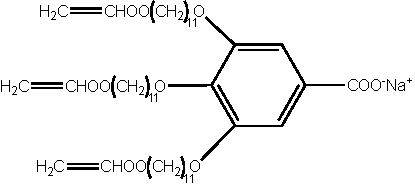
\includegraphics[width=\textwidth]{NaGA3C11.pdf}
  \caption{}\label{fig:monomer_structure}
  \end{subfigure}
  \begin{subfigure}{0.5\textwidth}
  \centering
  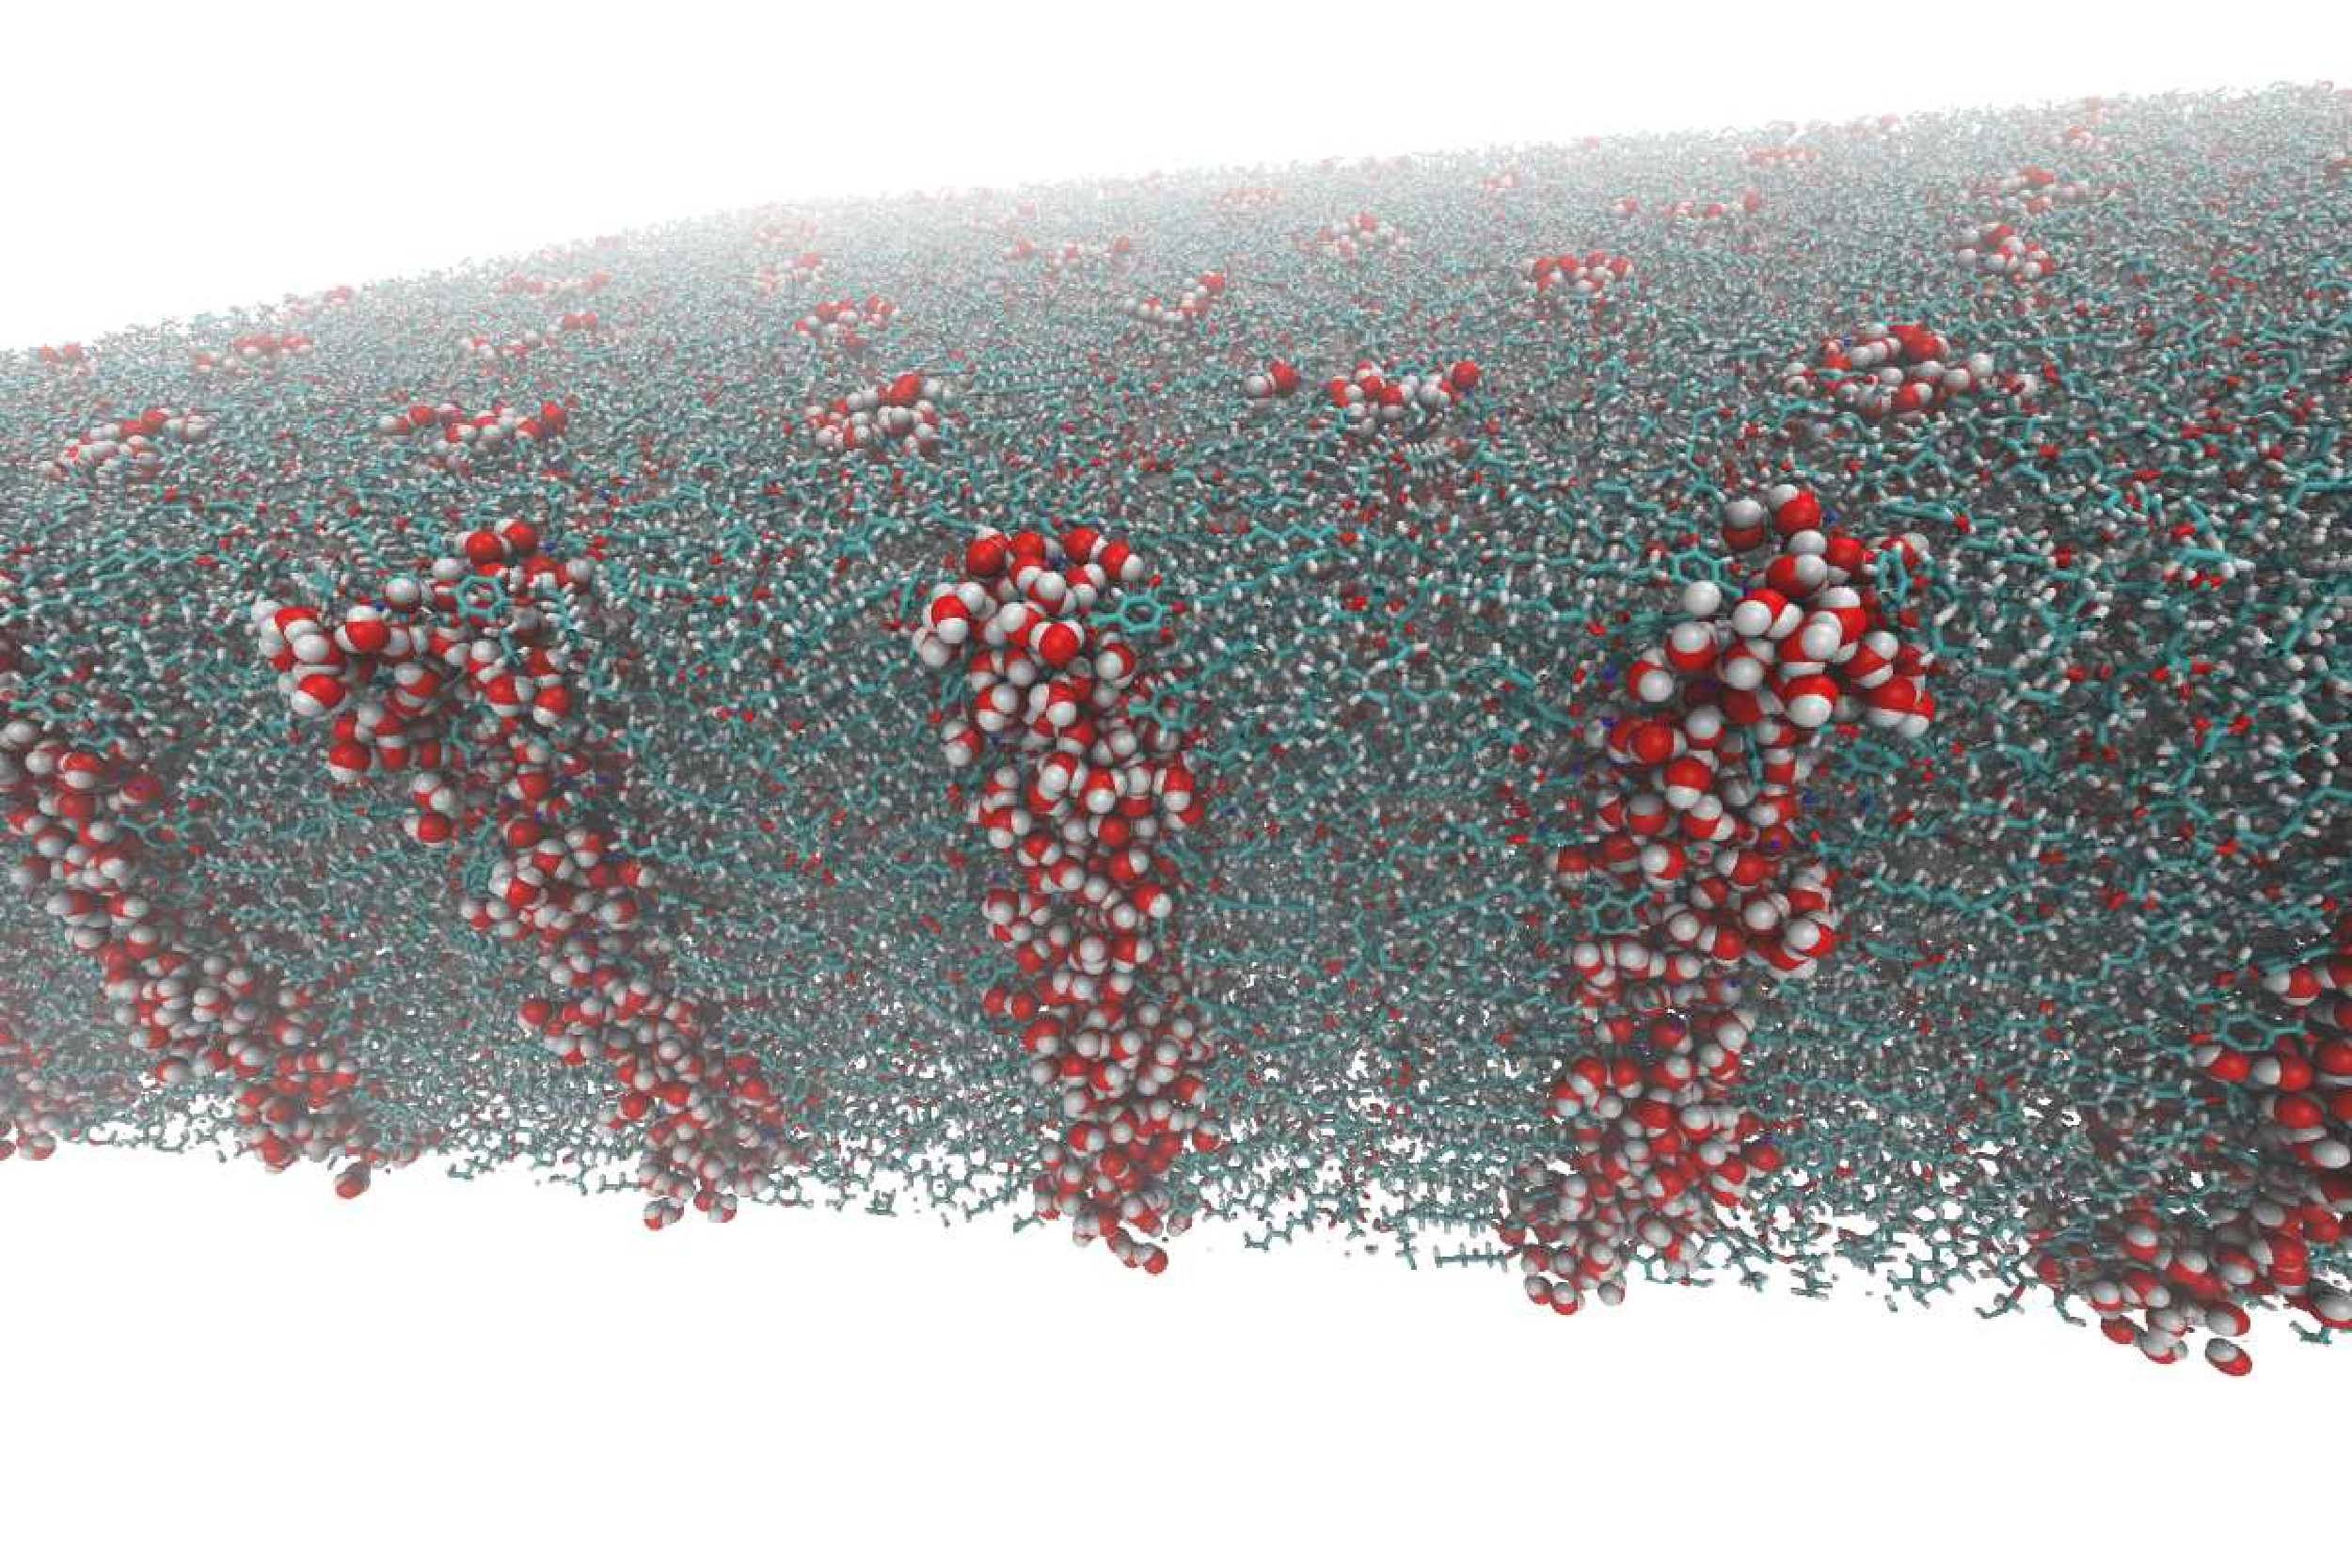
\includegraphics[width=\textwidth]{membrane_profile.pdf}
  \caption{}\label{fig:membrane_profile}
  \end{subfigure}
  \caption{(a) The wedge-shaped liquid crystal monomer Na-GA3C11 will form the inverted
  hexagonal phase in the presence of water where the carboxylate head groups occupy the
  pore centers. (b) A cross-section of a periodically replicated atomistic unit cell 
  used for simulations in this study reveals the membrane's aqueous, hexagonally packed,
  straight and uniform sized pores. Water present in the distal tail region is omitted 
  for clarity.}\label{fig:membrane_structure}
  \end{figure}
  
  We chose to study a subset of the 4 fastest moving solutes from our previous
  work: methanol, acetic acid, urea and ethylene glycol. For each solute we 
  created a separate system and to each system we added 6 solutes per pore 
  for a total of 24 solutes. This number of solutes per pore provides a balance
  of a low degree of interaction between solutes, since we are primarily interested 
  in solute-membrane interactions at present, as well as a sufficient amount of 
  data from which to generate statistics on the time scales which we simulate.
  Further details on the setup and equilibration of these systems are described in
  our previous work.\cite{coscia_chemically_2019}
  
  We extended the 1 $\mu$s simulations of our previous work to 5 $\mu$s in order
  to collect ample data. We simulated the system with a time step of 2 fs at a pressure
  of 1 bar and 300 K controlled by the Parrinello-Rahman barostat and the v-rescale 
  thermostat respectively. We recorded frames every 0.5 ns.
  
  We considered each system to be equilibrated when the solute partitioning between the 
  pore and tail region reached apparent equilibrium and use only data after that point
  in our analysis of solute kinetics. We plotted the solute partition versus time in
  Figure~\ref{S-fig:equilibration} of the Supporting Information in order to justify 
  our choice of equilibration times for each solute.

  \subsection{The Anomalous Diffusion Model}\label{method:model_sFBM}

  % BJC3: x --> z since I'm measuring diffusion in the z direction?
  % MRS4: reasonable change.  Or explicitly state that you will refer to the pore axis as x. 
  % BJC4: I think it'll be less confusing to me writing it to change it to z.
  Solutes in this system exhibit subdiffusive behavior, a type of anomalous diffusion.
  During an anomalous diffusion process, the mean squared displacement (MSD)
  does not grow linearly with time, rather it follows a power law of the form:
  \begin{equation} 
  \langle z^2(t) \rangle = K_{\alpha_d}t^{\alpha_d}
  \label{eqn:msd_form}
  \end{equation} 
  where $\alpha_d$ is the anomalous exponent and $K_{\alpha_d}$ is the generalized 
  diffusion coefficient. We only calculate MSD with respect to the solutes' center of
  mass $z$-coordinate, which is oriented along the pore axis. A value of $\alpha_d < 1$
  indicates a subdiffusive process, while values of $\alpha_d = 1$ and $\alpha_d > 0$ 
  are characteristic of Brownian and superdiffusive motion respectively.
  
  %BJC3: removed ensemble MSD because it's not used
  We analyzed the time-averaged MSD of the simulated trajectories by measuring
  all possible displacements over time lag $\tau$:
  \begin{equation}
  \overline{z^2(\tau)} = \dfrac{1}{T - \tau}\int_{0}^{T - \tau} (z(t + \tau) - z(t))^2 dt
  \end{equation}
  where T is the length of the trajectory. Note that only the \textit{ensemble} MSD
  will reproduce the form of Equation~\ref{eqn:msd_form} in all cases. 
  %MRS4: probably need to explain in what way it is non-ergodic below, and if this is the scenario that people should care about.
  %BJC4: reworded, defined ergodicity (usually called 'weak' ergodicity breaking in literature) and
  % explained why it's not important for this study.
  In a pure CTRW, for example, the power law distribution of trapping times leads to
  weak ergodicity breaking. The time-averaged MSD is linear while the ensemble averaged
  MSD has the form of Equation~\ref{eqn:msd_form}.~\cite{meroz_toolbox_2015} With power
  law trapping behavior, the time between hops diverges so there is no characteristic
  measurement time scale of solute motion. In fact, as measurement time increases, the 
  MSD of a CTRW tends to decrease, a phenomenon called aging, because trajectories 
  with trapping times on the order of the measurement time get incorporated into the 
  calculation.~\cite{bel_weak_2005} We chose to analyze just the time-averaged MSD 
  because, compared to the ensemble average, it is a more statistically robust measure
  of the average distance a solute travels over time. Although theoretically possible, we do
  not use the MSD to calculate $\alpha_d$ because we can extract the same parameter 
  with higher precision using the dwell time distributions as described below.
  
%  of the process is exhibits weak ergodicity breaking due to 
%  If the underlying subdiffusive process is not ergodic, like a pure CTRW, the time
%  averaged MSD becomes linear.
  
  \subsubsection*{Subordinated Fractional Brownian Motion}
  
  The solute motion in the system studied here may be consistent with 
  subordinated fractional Brownian motion (sFBM) where the parent process is FBM and 
  the leading process is a CTRW. We observe hopping and trapping which is consistent
  with a CTRW, along with negatively correlated hops which is consistent with FBM.  

  One can characterize a CTRW process by the parameters which describe its dwell 
  time and hop length distributions. We used the \texttt{ruptures} python package in 
  order to automatically identify mean shifts in solute trajectories, indicating hops.\cite{truong_ruptures:_2018} 
  We used the corresponding hop lengths and dwell times between hops to construct 
  empirical distributions.
  
  \textit{Dwell time distributions:} For subdiffusive transport, the distribution 
  of dwell times is expected to fit a power law distribution 
  proportional to $t^{-1-\alpha_d}$.~\cite{meroz_toolbox_2015}
  %BJC3: is it okay to leave above equation in line? Or should it get numbered?
  %BJC3: I added subscript d to the dwell time alpha because alpha is a standard parameter for power laws and levy stable distributions
% BJC3: following includes normalization constant 
%  of the form:
%  \begin{equation}
%  (\beta - 1)x_{min}^{\beta - 1}x^{-\beta}
%  \end{equation}  
%  where $\beta = (1 + \alpha)$ and $x_{min}$ is the smallest measured value of $x_i$.~\cite{meroz_toolbox_2015,clauset_power-law_2009}
%  proportional to $t^{-1-\alpha}$.~\cite{meroz_toolbox_2015}
  Because we are limited to taking measurements at discrete intervals dictated by the output 
  frequency of our simulation trajectories, we fit the empirical dwell times
  to a discrete power law distribution whose maximum likelihood $\alpha_d$ 
  parameter we calculated by maximizing the following likelihood function: 
  \begin{equation}
	\mathcal{L}(\beta) = -n\ln \zeta(\beta, t_{min}) -
	\beta\sum_{i=1}^{n} \ln t_i 
  \label{eqn:powerlaw_likelihood}
  \end{equation}
  where $\beta = 1 + \alpha_d$, $t_i$ are collected dwell time data points,
  $n$ the total number of data points, and $\zeta$ is the Hurwitz zeta function
  where $t_{min}$ is the smallest measured value of	$t$.~\cite{clauset_power-law_2009}
  
  In practical applications, the heavy tail of power law distributions can result in 
  arbitrarily long dwell times that are never observed in MD simulations. We can not
  observe dwell times longer than the length of a single trajectory. 
  % Could be an interesting factoid, but not necessary 
  % In fact, the longest dwell time observed by any solute in this study is X. 
  In order to directly compare our anomalous diffusion model to finite-length MD 
  trajectories we may need to bound the dwell time distribution. We do this by adding 
  an exponential cut-off to the power law so the dwell time distribution is 
  now proportional to $t^{-1 - \alpha_d}e^{-\lambda t}$.
  % of the form:
%  \begin{equation}  %BJC3: maybe make this equation in line? Else move regular power law to its own equation
%    p(t) \propto t^{-1 - \alpha}e^{-\lambda t}
%  \label{eqn:powerlaw_cutoff}
%  \end{equation}
  We determine MLEs of $\alpha_d$ and $\lambda$ by maximizing the likelihood function:~\cite{clauset_power-law_2009}
  \begin{equation}
    \mathcal{L}(\alpha_d, \lambda) = n(1 - \alpha_d)\ln\lambda - n\ln\Gamma(1 - \alpha_d, t_{min}\lambda) - \alpha_d\sum_{i=1}^{n}\ln t_i - \lambda\sum_{i=1}^n t_i
  \label{eqn:powerlaw_cutoff_likelihood}
  \end{equation}
  
  \textit{Correlated hop length distributions:} The marginal distribution of hops by solutes 
  undergoing an sFBM process is Gaussian, therefore we parameterize it by its standard deviation, 
  $\sigma$.~\cite{metzler_random_2000, metzler_anomalous_2014,neusius_subdiffusion_2009}
  The measured mean is always very close to zero so we assume that it is exactly zero
  in our time series simulations since we have no reason to expect drift in either direction.

  % BJC3: Making a logical argument regarding how we estimate H here is important
  % because I haven't seen anyone do it this way.
  sFBM implies that hops are correlated which we describe using the Hurst parameter, $H$. 
  The autocovariance function of hop lengths has the analytical form:~\cite{mandelbrot_fractional_1968}
  \begin{equation}
    \gamma(k) = \dfrac{\sigma^2}{2}\bigg[|k-1|^{2H} - 2|k|^{2H} + |k+1|^{2H}\bigg]
  \label{eqn:fbm_autocorrelation}
  \end{equation}
  where $\sigma^2$ is the variance of the underlying Gaussian distribution from which hops are
  drawn and $k$ is the time lag, or number of increments between hops. The hop autocorrelation
  function is simply Equation~\ref{eqn:fbm_autocorrelation} normalized by the variance. 
  When $H < 0.5$, hops are negatively correlated, when $H = 0.5$ we recover Brownian motion
  and when $H > 0.5$, one observes positive correlation between hops. There are many methods
  for estimating the Hurst parameter for a time series.~\cite{clegg_practical_2006} It can
  be a difficult task because Equation~\ref{eqn:fbm_autocorrelation} decays slowly to zero, 
  especially when $H > 0.5$, meaning one needs to study large time lags with high frequency.
  Fortunately (from a mathematical perspective), all of our solutes show anti-correlated motion, so most of the information in
  Equation~\ref{eqn:fbm_autocorrelation} is contained within the first few time lags (see 
  Figure~\ref{S-fig:hurst_autocorrelation} of the Supporting Information). Any hope of
  fitting longer time lags to our data is lost in the noise since the analytical values
  are so close to zero. Therefore, we obtained H by performing a least squares fit of 
  Equation~\ref{eqn:fbm_autocorrelation} to the first 10 lags of the empirically measured
  autocorrelation function.

  \subsubsection*{Subordinated Fractional L\'evy Motion}

  If the distribution of hops is not Gaussian, we can model them with the
  more general class of L\'evy stable distributions. For independent and identically
  distributed random variables, the generalized central limit theorem assures 
  convergence of the associated probability distribution function (PDF) to a 
  L\'evy stable PDF. \cite{klages_anomalous_2008} The characteristic equation which 
  describes the Fourier transform of a L\'evy stable PDF is:
  \begin{equation}
    p_{\alpha_h, \beta}(k;\mu,\sigma) =\exp\left[i\mu k - \sigma^{\alpha_h}|k|^{\alpha_h}\left(1 - i\beta\frac{k}{|k|}\omega(k, \alpha_h)\right)\right]
  \end{equation}
  where \\
  \[\omega(k, \alpha_h) = \begin{cases}
  	\tan{\frac{\pi \alpha_h}{2}} & \text{if}~\alpha_h \neq 1, 0 < \alpha_h < 2, \\
  	-\frac{2}{\pi}\ln |k| & \text{if}~\alpha_h = 1
  	 \end{cases}
  \]
  $\alpha_h$ is the index of stability or L\'evy index, $\beta$ is the skewness 
  parameter, $\mu$ is the shift parameter and $\sigma$ is a scale parameter. The most
  familiar case, and 1 of 3 that can be expressed in terms of elementary functions,
  is the Gaussian PDF ($\alpha_h$ = 2, $\beta$ = 0). We assume symmetric distributions
  centered about 0 implying that $\beta$ and $\mu$ are both 0.
  
  Assuming hops are correlated, solute behavior may be described by subordinated 
  fractional L\'evy motion (sFLM). The Hurst parameter can again be used to describe
  hop correlations because they share the same autocorrelation structure.~\cite{tikanmaki_fractional_2010}
  The autocovariance function for FLM is:
  \begin{equation}
    \gamma(k) = \dfrac{C}{2}\bigg[|k-1|^{2H} - 2|k|^{2H} + |k+1|^{2H}\bigg],
    ~C = \frac{E\big[L(1)^2\big]}{\Gamma(2H + 1)\sin(\pi H)}
    \label{eqn:flm_autocovariance}
  \end{equation}
  where $E\big[L(1)^2\big]$ is the expected value of squared draws from the 
  underlying L\'evy distribution, effectively the distribution's 
  variance.~\cite{bishwal_maximum_2011} In general, most L\'evy stable distributions
  have an undefined variance due to their heavy tails. However, normalizing
  Equation~\ref{eqn:flm_autocovariance} by the variance of a finite number of draws
  from a L\'evy stable distribution results in the same autocorrelation structure as FBM.
  See Section~\ref{S-section:H_estimate} of the Supporting Information for numerical
  simulations illustrating this point.  % BJC3: could use another reference proving mathematically what I show numerically
  
  Analogous to power law dwell times, the heavy tails of L\'evy stable 
  hop length distributions result in rare but arbitrarily long hops. These long
  and unrealistic hops result in over-estimated simulated MSDs. We observe that
  the distribution of hops observed in our MD simulations are well approximated 
  by L\'evy stable distributions close to the mean, but they significantly under-sample
  the tails. We chose to truncate the L\'evy stable distributions based
  on where the theoretical probability distribution function (PDF) starts to 
  deviate from the empirically measured PDF (see Section~\ref{S-section:truncation}
  of the Supporting Information).
  
  % BJC3: maybe a table of cut-offs used here. We will see how close they are. Might
  % use the same for all.

  %MRS4: should be more clear which of the two kinetics scenarios this next assumption applies to
  %BJC4: changed title to clarify that this is anomalous diffusion
  \subsubsection*{Multiple Anomalous Diffusion Regimes}
  
  We observe different dynamical behavior when solutes move while inside 
  the pore versus while in the tail region. This inspired two anomalous diffusion 
  models of varying complexity. We created a simple, single mode model with a single 
  set of parameters fit to solute trajectories.
%  $\alpha$, $\sigma$, $H$ and, when the truncated power law is used, $\lambda$ parameters
%  fit to solute trajectories.
  Our second, two mode model assigns a set of parameters to each of 2 modes based
  on the solute's radial location. Solutes in mode 1 are in the pore region, defined
  %MRS4: some justification on why 0.75 vs. any other cutoff.
  %BJC4: I justified sentence after next. 
  as less than 0.75 nm from any pore center. All else are in mode 2, the tail region. 
  We determined this cut-off by maximizing the difference in dynamical behavior as 
  described in our previous work.~\cite{coscia_chemically_2019} Unfortunately, 
  there were not enough sufficiently long sequences of hops in each mode to reliably
  calculate a Hurst parameter for each mode so we used the Hurst parameter from the 
  single mode model for both modes of the two mode model.
  
  % BJC3: A small figure describing above might be useful, or maybe point to a figure in supporting info
 
  For the two mode model, we defined a transition matrix describing the rate at
  which solutes moved between the tail and pore region. We assumed Markovian transitions
  between modes, meaning each transition had no memory of previously visited modes. 
  We populated a 2$\times$2 count matrix by incrementing the appropriate entry by 1 each time step. 
  For example, if we observed the solute in the tails followed by a transition to 
  the pores, we incremented the $(2, 1)$ entry of the count matrix by 1. We generated
  the transition probability matrix from the count matrix by normalizing the 
  entries in each row so that they summed to unity.
 
  %MRS4: Do you assume Markovian behavior in transitions between the states?  Be explicit.
  %BJC4: Yes, added sentence directly after thesis above
  
  \subsubsection*{Simulating Anomalous Diffusion}

  We simulated models with all combinations of the types of dwell and hop length
  distributions described above, which are summarized in Table~\ref{table:anomalous_models}.
  All models include correlation between hops.
  %MRS4: not abbreviations are not necessarily defined: should be defined above, perhaps? (i.e. we will refer X as 'sFBMcut')
  %BJC4: made table
  \begin{table}[!htb]
	  \centering
	  \begin{tabular}{|c|c|c|}
	  \hline
	  Dwell Distribution                & Hop Length Distribution & Abbreviation \\
	  \hline
      Power Law                         & Gaussian                & sFBM         \\
      Power Law w/ Exponential Cut-off  & Gaussian                & sFBMcut      \\
      Power Law                         & L\'evy Stable           & sFLM         \\
      Power Law w/ Exponential Cut-off  & L\'evy Stable           & sFLMcut      \\
	  \hline
	  \end{tabular}
	  \caption{We tested models with various modifications to the dwell and hop
	  length distributions. We incorporate correlation structure into all models.}\label{table:anomalous_models}
 \end{table}

  % BJC3: will need to modify this text to reflect different lengths of simulations
  For each solute, we simulated 10,000 anomalous diffusion trajectories of length
  $T_{sim}$ in order to directly compare our model's predictions to MD simulations.
  $T_{sim}$ varied due to differing solute equilibration times. We constructed 
  trajectories by simulating sequences of dwell times and correlated hop lengths
  generated based on parameters randomly chosen from our bootstrapped parameter 
  distributions. We propagated each trajectory until the total time equaled or 
  exceeded $T_{sim}~ \mu$s, then truncated the last data point so that the total 
  time exactly equaled $T_{sim}~ \mu$s since valid comparisons are only possible 
  between fixed length sFBM simulations. 
  % BJC4: removed following sentence because I talk about aging above
  %The power law dwell time behavior gives rise to the aging phenomenon, embodied by a 
  %decrease in MSD with measurement time.~\cite{neusius_subdiffusion_2008,metzler_anomalous_2014}
  We reported the time-averaged MSD after time lags 40\% the length of the trajectory
  with corresponding 95\% confidence intervals.
  When simulating 2 mode models, we determined the state sequence based on random 
  draws weighted by the appropriate row of the probability transition matrix. We 
  drew hops and dwells based on the current state of the system. Since we calculated
  the transition probabilities from a finite data set, they have an associated 
  uncertainty which we 
  %MRS4: not quite sure what you mean by incorporating uncertainty. 
  %BJC4: Added comment about having a finite amount of data with which to create transition matrix. Therefore it is uncertain
  incorporated by re-sampling each row from a two dimensional Dirichlet distribution
  (also called a beta distribution for the 2D case) with concentration parameters 
  defined by the count matrix.~\cite{bacallado_bayesian_2009}

  %BJC4: already said this earlier
%  We used a single Hurst parameter to describe
%  correlation between hops, independent of the solute's mode. Ideally, each mode
%  would have its own Hurst parameter, but we did not observe enough long sequences
%  of uninterrupted time spent in each mode with which to generate robust
%  autocorrelation functions. 
  
  %We also projected MSDs out to 1 second for each solute. % BJC3:??
  %BJC3: not sure how to cite fbm
  We used the python package \texttt{fbm} to generate exact simulations of FBM and our
  own python implementation of the algorithm by Stoev and Taqqu to simulate FLM.
  \cite{stoev_simulation_2004} Note that, to our knowledge, there are no known exact
  simulation algorithms for generating FLM trajectories, however, the algorithm
  we used sufficiently approximates draws from the marginal distribution and 
  reasonably approximates the correlation structure. We added an empirical correction
  to enhance the accuracy of the correlation structure (see Section~\ref{S-section:flm_correlation}
  of the Supporting Information for validation of the approach).
  
%  When simulating 5 $\mu s$ FLM trajectories, we limited the maximum hop length to
%  be no larger than the largest hop observed in our MD simulations. L\'evy stable 
%  distributions often have heavy tails and an undefined variance which can give 
%  rise to arbitrarily long particle displacements. We do not observe hops longer 
%  than x nm in our simulations which emphasizes that these distributions are only 
%  an approximation. We avoid enormous and unrealistic hops problem by truncating 
%  the tails of the distribution.

%  An important feature 
%  of L\'evy distributions is their heavy tails. Generally, a lower L\'evy index is 
%  characteristic of heavier tails, meaning higher probabilities of extremely large jumps.
%  In practical applications these extremely large hop lengths are unrealistic, especially
%  when comparing to MD.

%  BJC4: I already said this above
%  When simulating MD-length FLM trajectories, we limited the maximum hop length based on where
%  the empirical hop distribution began to significantly under-sample the theoretical
%  maximum likelihood estimate (MLE) L\'evy stable distribution (see 
%  Section~\ref{S-section:truncation} of the Supporting Information).

%  For our 1 second simulations, we limited the maximum hop length to that seen by
%  the same solute undergoing Brownian motion in an unconfined aqueous environment. 
%  We have no reason to believe there is any kind of facilitated diffusion, so 
%  excursions characteristic of Brownian motion represent a reasonable upper limit
%  on hop lengths. To determine these limits we placed 24 solutes in a cubic box of 
%  water, 4 nm on each side. We allowed the solutes to diffuse for 100 ns, more than
%  ensuring the mean squared displacement entered a linear regime. We recorded the largest
%  observed hop length over a 0.5 ns time lag. 

  \subsection{Markov State-Dependent Dynamics}\label{method:MSMs}  

  A Markov state model (MSM) decomposes a time series into a set of discrete states
  with transitions between states defined by a transition probability matrix, $T$,
  which describes the conditional probability of jumping to a specific state given
  the previously observed state.~\cite{pande_everything_2010,wehmeyer_introduction_2018}
  Software packages such as MSMbuilder~\cite{beauchamp_msmbuilder2:_2011} and 
  pyEMMA~\cite{scherer_pyemma_2015} provide work flows capable of featurization and
  dimensional reduction which are often necessary to identify representative states.

  In this work, we define a total of 8 discrete states based on the 3 trapping
  mechanisms observed in our previous work. Therefore, there is no need to 
  apply any algorithmic approaches to identify and decompose our system into 
  discrete states. The states we have chosen include all combinations of trapping
  mechanisms in the pore and out of the pore (see Table~\ref{table:states}). We use
  the same radial cut-off (0.75 nm) as in the anomalous diffusion model to differentiate
  the pore and tail region. These state choices assume that there are no significant
  kinetic effects resulting from solute conformational changes or pore size fluctuations,
  an assumption that may be relaxed in future work.
  
  \begin{table}[!htb]
	  \centering
	  \begin{tabular}{|l|l|}
	  \hline
	  1. In tails, not trapped                     & 5. In pores, not trapped                     \\
	  2. In tails and hydrogen bonding             & 6. In pores and hydrogen bonding             \\
	  3. In tails and associated with sodium       & 7. In pores and associated with sodium       \\
	  4. In tails, hydrogen bonding and associated & 8. In pores, hydrogen bonding and associated \\
	  \hline
	  \end{tabular}
	  \caption{We defined 8 discrete states based on all combinations of previously observed solute
	  trapping mechanisms}\label{table:states}  
	  %BJC3: the caption will depend on the journal. I don't
	  % like that J Phys Chem B forces the captions as titles, but if we choose them I think it would
	  % be cleaner to make the caption more title-like.
  \end{table}
  
  We constructed the state transition probability matrix, $T$, based on observed solute trajectories.
  Using methods described in our previous work, we determined each solute's radial location 
  and which, if any, trapping mechanisms affected it at each time step, then assigned the 
  observation to a specific state according to the definitions in Table~\ref{table:states}.~\cite{coscia_chemically_2019}
  Analogous to the mode transition matrix in Section~\ref{method:model_sFBM}, and based on
  the current and previous state observation, we incremented the appropriate entry of an
  $n~\times~n$ count matrix by 1, where $n$ is the number of states.
  
  %MRS4: here, be more explicit you are testing the validity of the Markovian approximation on the molecular data.
  %BJC4: Tried to clarify in thesis statement. Let me know if you think it needs more
  We verified the Markovianity of state transitions by solutes in our MD simulations 
  by analyzing the empirically measured transition matrix. An important condition
  of a Markov process is the satisfaction of detailed balance:
  \begin{equation}
  T_{i,j}P_i(t=\infty) = T_{j,i}P_j(t=\infty)
  \end{equation}
  where $P$ is the equilibrium distribution of states. In other words, the number of
  transitions from state $i$ to $j$ and from state $j$ to $i$ should be equal. A second
  test is to verify that $T$ holds up to coarser time scales. As long as solutes
  sufficiently sample the states in Table~\ref{table:states}, $T$ should be invariant
  with time.~\cite{swope_describing_2004} We verified these properties 
  in Section~\ref{S-section:markov_validation} of the Supporting Information.
  
  % BJC3: This explanation is in previous section
  %For example, if 
  %we observed state 1 followed by a transition to state 3, we increment the $(1, 3)$ entry
  %of the count matrix by 1. We generate the transition probability matrix from the count matrix by 
  %normalizing the entries in each row so that they summed to unity.
  
  Adding to the standard MSM framework, we incorporated the dynamics of the solutes
  within each state as well as the dynamics of state transitions, which includes the
  overall configurational state of the solute and it's environments. 
  While MSMs are often used to gauge equilibrium populations of various states, adding 
  %MRS4: it's not just ``dynamics'', though, it's a specific subset of the dynamics.  
  % And one could argue that the MSMs are being added to the dynamics, since the time trace is the desired output, 
  % rather than the output one usually gets from MSMs.
  %BJC4: made more specific with 'state-dependent dynamics' instead of just 'dynamics'
  %BJC4: confusion here
  state-dependent dynamics allows us to more accurately simulate solute trajectories.
  %BJC4: I said below already
  Hence we distinguish our model from MSMs by referring them as Markov State-Dependent
  Dynamical Models (MSDDMs). 
  
  We recorded the $z$-direction displacement at each time step in order to construct 
  individual emission distributions for each state and transition between states. 
  This results in 64 distinct emission distributions with some far more populated than
  others. We modeled all of the emission distributions as symmetric L\'evy stable 
  distributions in order to maintain flexibility in parameterizing the distributions.
  
  We observed negatively correlated hops within each state and among transitions between
  states. We can use the Hurst parameter to describe this negative time series correlation
  however, there is not sufficient data to accurately measure a Hurst parameter for 
  each type of transition. We avoided this problem by treating transitions as correlated
  emissions from a single L\'evy stable distribution. This reduces the number of emission
  distributions from 64 to 9 (1 for each state and 1 for transitions between states).
  
  We simulated realizations of the MSDDM using the probability transition matrix and 
  emission distributions. For each trajectory simulated, we chose an initial state
  randomly from a uniform distribution. We generated a full state sequence by randomly
  drawing subsequent states weighted by the rows of the probability transition matrix
  corresponding to the particle's current state. Again, because we are working with a
  finite data set, we incorporated uncertainty into the rows of the transition matrix 
  by resampling them from a Dirichlet distribution. For each same-state subsequence of
  the full state sequence, we simulated an FLM process using the Hurst parameter of that
  state and the parameters of the corresponding emission distribution. Independently, 
  we simulated the transition between each same-state sequence with an FLM process 
  based on the Hurst parameter of transition sequences and the parameters of the 
  single transition emission distribution. We used the same FLM simulation procedure
  described in Section~\ref{method:model_sFBM}.

%  corresponding emissions from the rows of the probability transition matrix and the 
%  appropriate emission distribution respectively. We added correlation between transitions
%  as well as to sequences of emissions while dwelling in specific states using the FLM
%  simulation procedure described in Section~\ref{method:model_sFBM}.

  \subsection{Solute Flux}\label{method:mfpt}
  
  We determined the rate at which solutes cross macroscopic-length pores based on the
  Hill relation:~\cite{hill_free_1989}
  \begin{equation}
  J = \frac{1}{MFPT}
  \label{eqn:hill_relation}
  \end{equation}
  where $J$ is the single particle solute flux and MFPT refers to the mean first passage
  time. For particle concentrations higher than 1 at the pore entrance, one can multiply
  Equation~\ref{eqn:hill_relation} by the total number of particles to get the total flux.
  In the context of our work, the MFPT describes the average length of time it takes a particle
  to move from the pore entrance to the pore exit. 
  
  We generated particle trajectories, parameterized with the above models, in order
  to construct a distribution of first passage times across a membrane pore of length $L$.
  We simulated 50000 trajectory realizations, released at the pore entrance ($z=0$). In the case of 
  uncorrelated hops, one can continuously draw from the hop length distribution until 
  $z \geq L$ (or $-L$ for the sake of computational efficiency). The length of time 
  between the last time the particle crossed $z=0$ and the end of the trajectory gives a 
  single passage time. When particle hops are correlated, as they are in all cases of
  this work, we cannot continuously construct the particle trajectories. Rather, we must
  generate trajectories of length $n$ and measure the length of the sub-trajectory 
  which traverses from $0$ to $L$ without becoming negative.
  %BJC4: below is only necessary if you the mean of the distribution exists.
  %It is important to choose a value of $n$ sufficiently
  %large that all trajectories reach $L$, or else the mean first passage time will 
  %be underestimated. 
  
  We calculated the expected value of analytical fits to the passage time distributions
  in order to determine the MFPT for a given solute and pore length. One should not 
  use the mean of the empirical passage time distribution because it is highly likely
  that the true MFPT will be underestimated unless 100\% of a very large number of 
  trajectories reach $L$. If a trajectory does not reach $L$ within $n$ steps, it is
  possible that a very long passage time has been excluded from the distribution.
  
  %BJC4: can probably delete this paragraph
%  We are unaware of an analytical passage time distribution which describes our 
%  geometry. The setup of our system is consistent with a one dimensional interval 
%  with two absorbing boundaries. In the absence of an external force and with a constant
%  diffusion coefficient, $D$, the MFPT is simply:
%  \begin{equation}
%  T = \frac{z_0(L - z_0)}{2D}
%  \end{equation}
%  where $z_0$ is the initial position of particle trajectories.~\cite{gitterman_mean_2000}
%  Of course that implies a conventional MFPT of 0 since particles overwhelmingly exit the
%  pore at $z=0$. Therefore, we chose only to include trajectories in the MFPT calculation 
%  which cross the boundary at $L$. We are unaware of an analytical form of the MFPT or 
%  the distribution of passage times describing our system even in the simplest case of 
%  Brownian increments. %BJC4: still digging for an analytical solution. Rich said the 
%  %'marathon' runner problem might give a solution. It may be the same as the distribution
%  % of runners crossing the finish line
  
  To come up with an analytical equation describing the passage time distributions, 
  one can frame the problem as a pulse of particles instantaneously released at the 
  pore inlet ($z=0$) which moves at a constant velocity and spreads out as it 
  approaches $L$. This gives results equivalent to if we had released each particle
  individually and then analyzed the positions of the ensemble of trajectories as 
  a function of time. 
  
  To derive an analytical equation, first consider an initial pulse spreading out 
  over time with a fixed mean. We can solve for the time-dependent probability density
  of particle positions by solving the one dimensional diffusion equation:
  \begin{equation}
  \frac{\partial p}{\partial t} = D \frac{\partial^2 p}{\partial z^2}
  \end{equation}
  The appropriate initial and boundary conditions are:
  $$BC1: t > 0, z = \infty, p = 0$$
  $$BC2: t > 0, z = 0, \frac{\partial p}{\partial z} = 0$$
  $$IC: t = 0, c = M\delta(z)$$
  where $M$ is the total number of particles in the system. It has been shown 
  elsewhere that the solution to this equation is:~\cite{cussler_diffusion:_2009}
  \begin{equation}
  p(z, t) = \frac{1}{\sqrt{4 \pi D t}}exp\bigg(\frac{-z^2}{4Dt}\bigg)
  \end{equation}
  We can make the substitution $z = z - vt$, where $v$ represents a constant average
  velocity, in order to linearly shift the mean as a function of time:
  \begin{equation}
  p(z, t) = \frac{1}{\sqrt{4 \pi D t}}exp\bigg(\frac{-(z - vt)^2}{4Dt}\bigg)
  \end{equation}
  One can track the fraction of particles, $F$, that have crossed the pore 
  boundary by integrating:
  \begin{equation}
  F(t) = \int_L^\infty p~dz = erfc\bigg(\frac{L - vt}{2\sqrt{D t}}\bigg)
  \end{equation}
  where $L$ is the pore length. This represents the cumulative first passage 
  time distribution so we take its derivative in order to arrive at the first
  passage time distribution:
  \begin{equation}
  P(t) = -\frac{1}{\sqrt{\pi}}e^{-(L - vt)^2 / (4Dt)}\bigg(-\frac{D(L - vt)}{4(Dt)^{3/2}} - \frac{v}{2\sqrt{Dt}}\bigg)
  \label{eqn:passage_times}
  \end{equation} 
  where the only free parameters for fitting are $v$ and $D$. We calculated the
  expected value of Equation~\ref{eqn:passage_times} in order to get the MFPT.
  
  We used the ratio of solute fluxes in order to determine membrane selectivity, $S$,
  towards solutes. Selectivity of solute $i$ versus $j$ is defined in terms of the
  ratio of solute permeabilities, $P$:~\cite{guo_pervaporation_2004}
  \begin{equation}
  S_{ij} = \frac{P_i}{P_j}
  \end{equation}
  We can relate this to solute flux using Kedem and Katchalsky's equations for 
  solvent volumetric flux, $J_v$, and solute flux, $J_s$:~\cite{kedem_permeability_1963}
  %al-zoubi_rejection_2007 clarifies that these equations can be used for nanofiltration, ultrafiltration etc. by treating the membrane as a black box subject to irreversible thermodynamics.
  \begin{equation}
  J_v = L_p(\Delta P - \Delta \pi)
  \end{equation} 
  \begin{equation}
  J_s = P_s \Delta C + (1 - \sigma)CJ_v
  \label{eqn:solute_flux}
  \end{equation}
  where $L_p$ is the pure water permeability, $\Delta P$ and $\Delta \pi$ are the 
  trans-membrane hydraulic and osmotic pressure differences, $\sigma$ is the reflection
  coefficient, $P_s$ is the solute permeability, $\Delta C$ is the trans-membrane
  solute concentration difference and $C$ is the mean solute concentration. Since our
  simulations do not include convective solute flux, we eliminate the second term 
  of Equation~\ref{eqn:solute_flux} which allows us to derive a simple expression
  for selectivity in terms of solute flux:
  \begin{equation}
  S_{ij} = \frac{J_i / \Delta C_i}{J_j / \Delta C_j}
  \label{eqn:selectivity}
  \end{equation}
  
  
%    $$ A_i = \frac{J}{(\Delta P - \Delta \pi)} $$
%  $$ S = \frac{A_i}{A_j} for a given pore length, L$$
%  $$J = A(\Delta P - \Delta \pi)$$
%  $$A = \frac{P_i}{L} $$
%  $$P_i = \frac{flux}{drivingforce \cdot L} [=] \frac{particles}{s \cdot bar \cdot L}$$
  
  %BJC4: we have better ways of getting peaks now
%  In the absence of an analytical equation for the MFPT, we instead report the location of
%  the peak of the passage time distribution. This has the added advantage of treating
%  cases where the passage time distribution diverges and no mean exists. While we will
%  call the peak in the distribution the MFPT, it is important to recognize that this 
%  value is more representative of a typical passage time rather than a mean. 
  
  % BJC: concentration profile stuff
%  One would then segment the trajectory
%  each time it crosses $0$ and reflect all of the negative trajectories. The ensemble of
%  trajectories is consistent with the fraction of partic
  
  \section{Results and Discussion}
  
  %BJC4: Not sure if I should start by commenting on the stationarity of the 
  %solute trajectories. I talk about it when I start validating with the train/test procedure.
  
%  \subsection{Stationarity of Solute Trajectories}\label{section:stationarity}
%  %BJC4: Maybe re-theme the section: applicability of model
%  
%  Before applying the model, it is important to analyze the MD trajectories
%  themselves in order to understand what conclusions one could reasonably to 
%  draw by applying these models. 
%  
%  %BJC4: this might belong with validation.
%  We observe that in many cases, the distribution of solutes within the membrane
%  evolves slowly with time. We defined the perceived equilibration time point 
%  for each solute based on the time at which the number of solutes inside the
%  pores and tails stabilized. Nonetheless, we observe evidence of non-stationary
%  solute behavior after equilibration on the $\mu$s timescale. In Table \_\_, we compare the MSD of the 
%  solutes calculated using trajectory data from the first and second halves of the
%  equilibrated simulation time. Ethylene glycol and methanol, show considerable
%  differences in their MSDs. Although the MSD calculated from both halves of the 
%  acetic acid trajectories are similar, their shapes are considerably different 
%  (see SI). Urea is the only solute in this study that demonstrates satisfactory
%  stationarity on the 5 $\mu$s timescale.
%  
%  The non-stationary behavior of each solute presents itself in different ways.
%  On average, methanol molecules in the tails appear to be drifting further 
%  away from the pore center with time. Ethylene glycol appears to experience an
%  increased incidence of long trapping times. The partition of acetic acid 
%  between the pores and tails oscillates slowly over time. These problems probably
%  cannot be addressed without more simulation time or additional solute trajectories. 
%  
%  In light of these observations, we chose to demonstrate the performance and insights
%  that could be gained from our models using all of solutes with complete data sets
%  collected after the perceived equilibration time. However, we only use urea to 
%  validate the model's predictive power and to estimate solute flux.
%    
%  There are a couple of ways to address this issue in the long term. The simplest
%  approach is to run the MD simulations longer. This option is likely not feasible
%  because the equilibration timescale in these systems is unknown for most of 
%  the solutes in the study, even after consider computational effort. A more 
%  sustainable approach, which would help screen any solute of interest, would 
%  require us to learn the equilibrium distribution of solutes in the membrane
  
  \subsection{Anomalous Diffusion Modeling}\label{section:sFBM}

  The evidence suggests that solutes in this system can be well-modeled by subordinated
  fractional Brownian motion. The solutes clearly perform jumps after periods of relative
  immobility (see Figure~\ref{fig:solute_trajectories} for example). The near-Gaussian distribution
  of jump lengths and power law distribution of dwell times are both characteristic of 
  CTRWs (Figures~\ref{fig:hop_distribution_comparison} and~\ref{fig:powerlaw}). The apparent
  anti-correlation between hops suggests a fractional diffusion process is subordinate to the
  CTRW. We believe the subordinated process is FBM because its analytical correlation 
  structure is close to that observed in our simulation (Figure~\ref{fig:hop_acf}). FBM
  is common in crowded viscoelastic environments where motions are highly influenced by
  the motion of surrounding components, such as monomer tails in our case.~\cite{ernst_fractional_2012}
  The parameter estimates describing our 1 and 2 mode models are summarized in 
  Tables~\ref{table:sfbm_params} and~\ref{table:sfbm_params_2mode} (also trying it out in 
  Figures~\ref{fig:radars} and~\ref{fig:radars_nolines})
  
  \begin{figure}
  \centering
  %BJC3: included radial distance from pore center because I could. But does that make it look bad?
  % /figures/solute_trajectories.py
  \begin{subfigure}{0.45\textwidth}
  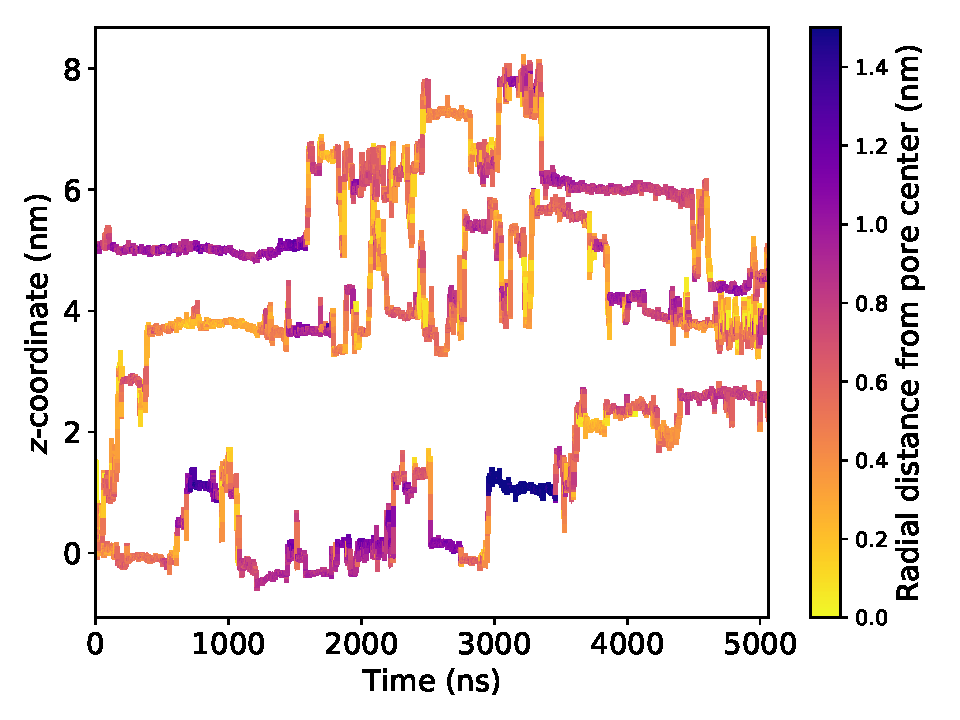
\includegraphics[width=\textwidth]{URE_trajectories.pdf}
  \caption{}\label{fig:solute_trajectories}
  \end{subfigure}
  % Next 3: /figures/sfbm_distributions
  \begin{subfigure}{0.45\textwidth}
  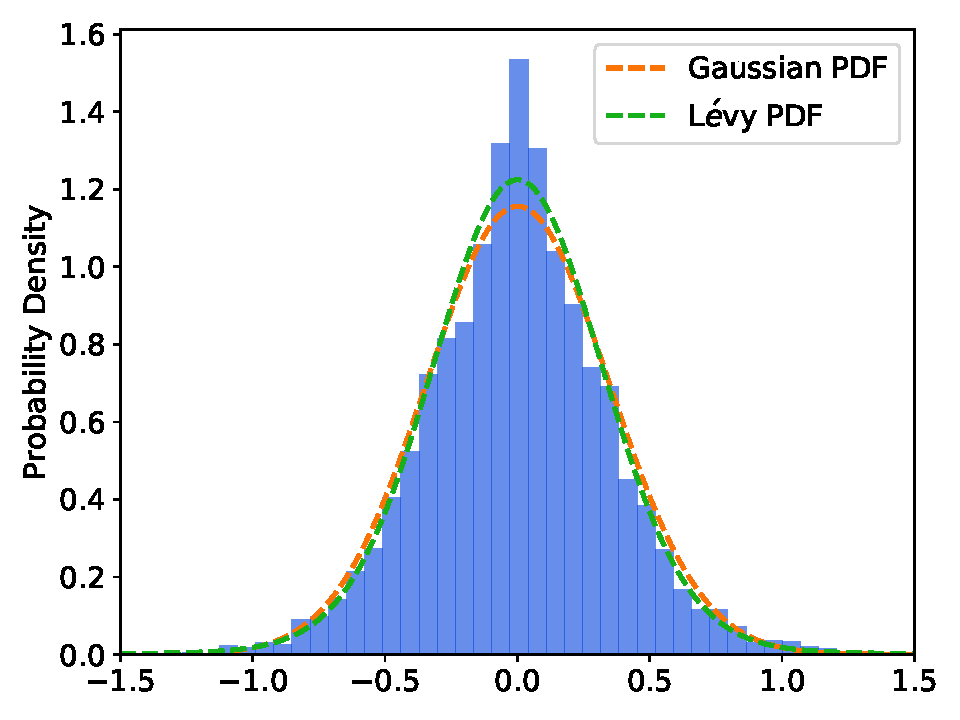
\includegraphics[width=\textwidth]{gaussian_levy_comparison_anomalous_GCL.pdf}
  \caption{}\label{fig:hop_distribution_comparison}
  \end{subfigure}
  \begin{subfigure}{0.45\textwidth}
  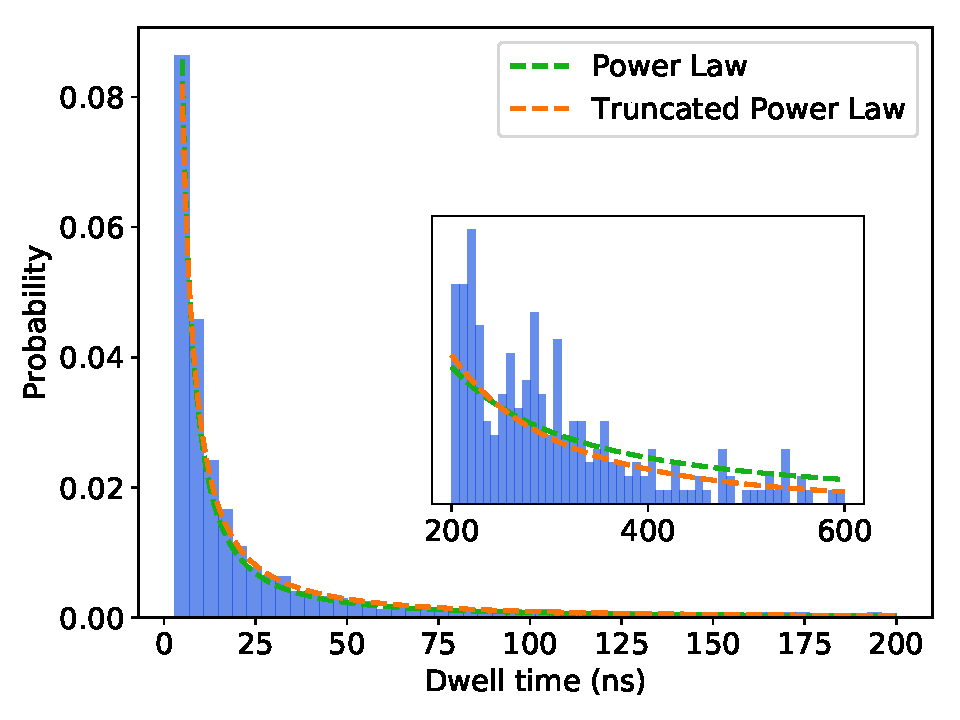
\includegraphics[width=\textwidth]{URE_powerlaw.pdf}
  \caption{}\label{fig:powerlaw}
  \end{subfigure}
  \begin{subfigure}{0.45\textwidth}
  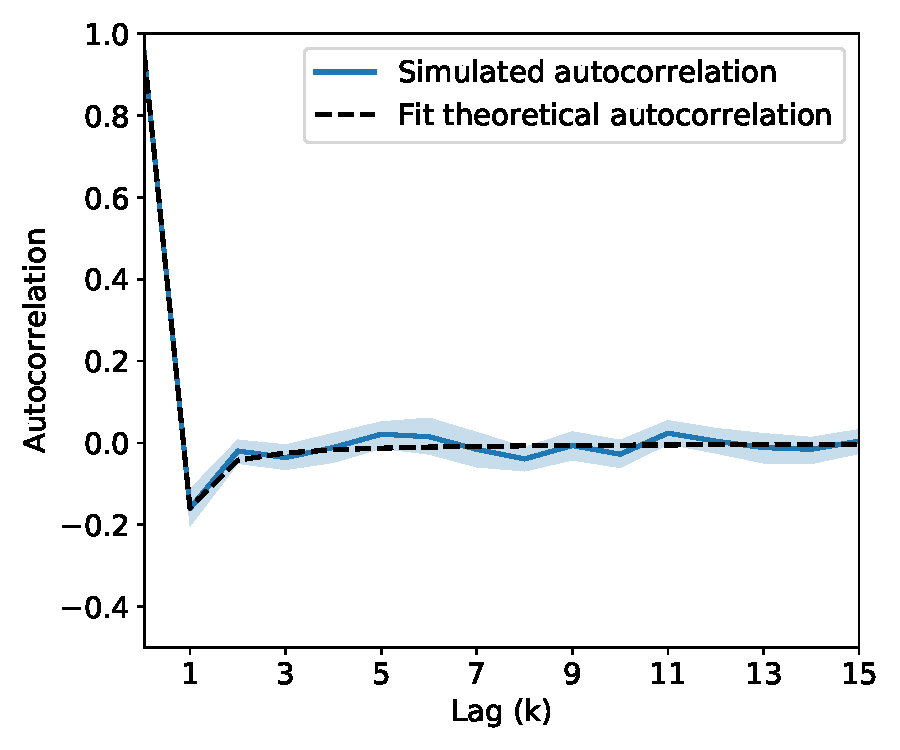
\includegraphics[width=\textwidth]{URE_hop_acf.pdf}
  \caption{}\label{fig:hop_acf}
  \end{subfigure}
  \caption{(a) Urea exhibit hops between periods of entrapment, characteristic of a CTRW. 
  (b) The distribution of hop lengths fits well to a Gaussian as well as a more general L\'evy 
  stable distribution. The L\'evy stable distribution does a better job of capturing the 
  heavier tails and increased density near 0. (c) The distribution of dwell times is fit
  well by a power law but it may over-estimate the probability density at long dwell times.
  A power law truncated with an exponential cut-off may better describe the probability of
  long dwell times in our simulations. (d) The hops are negatively correlated to their previous
  hop. In combination, (a) -- (d) support modeling solutes as subordinated fractional Brownian
  motion. The behavior shown by urea in this figure is common to all solutes in this study.}\label{fig:anticorrelated_hops}
  %MRS4: are there similar figures in the supporting information.
  %BJC4: no but I can make them
  \end{figure}
  
  We modeled the distributions of hop lengths in two ways. First, we assumed the 
  distribution to be Gaussian since it is possible to exactly simulate realizations of
  fractional Brownian motion. Second, we fit the distributions to L\'evy stable 
  distributions since it is more general than the Gaussian distribution. We plotted
  the MLE fits of both on top of urea's hop length distribution in 
  Figure~\ref{fig:hop_distribution_comparison}. The L\'evy distribution does a better
  job capturing the somewhat heavy tails and high density near 0 of the hop length distribution.
  However, since there are no known exact simulation techniques for generating 
  realizations of fractional L\'evy motion, we must evaluate whether this more general
  fit is worthwhile. 
  
  We also modeled the distribution of dwell times in two ways. First, we assumed pure
  power law behavior since it is consistent with most theoretical descriptions of CTRWs.
  The data fits well to this model at short dwell times but the density of long dwell
  times is over-estimated. In our second approach, we truncate the power law distribution
  with an exponential cut-off, lowering the probability of extremely long dwell times. 
  We demonstrate this effect in the inset to Figure~\ref{fig:powerlaw}, where the
  density of the truncated power law drops below that of the pure power law and tends towards
  0 near a dwell time of 250 ns.
  
  % BJC3: is it worth trying to combine these tables?
  % BJC: note to self -- modes are flipped in simulation output because 
  % physical.partition() sets mode as booleans and when r <= 0.75, in-pore is True (1) instead of 0. 
  \begin{table}[h]
  \centering
  \begin{tabular}{|M{2cm}|M{1.65cm}|M{1.95cm}|M{1.95cm}|M{1.95cm}|M{1.95cm}|}
  \hline
  1 Mode Model  & Parameters                & Urea         & Ethylene Glycol &   Methanol   & Acetic Acid  \\\hline
  Dwell         & $P(\alpha_d)$             & 0.57         & 0.62            & 0.62         & 0.45         \\\cline{2-6}
  Distributions & $P_T(\alpha_d, \lambda)$  & 0.40, 0.0024 & 0.47, 0.0030    & 0.44, 0.0040 & 0.08, 0.0033 \\\hline
  Hop           & $\mathcal{N}(\sigma)$     & 0.33         & 0.34            & 0.35         & 0.27         \\\cline{2-6}
  Distributions & $L(\sigma, \alpha_h)$     & 0.21, 1.84   & 0.23, 1.92      & 0.22, 1.80   & 0.16, 1.72   \\\hline
  Correlation   & $\gamma(H)$               & 0.37         & 0.40            & 0.30         & 0.34         \\
  \hline 
  \end{tabular}
  \caption{To create a 1 mode model for each solute, we parameterized a pure power
  law ($P(\alpha_d)$) and a truncated power law ($P_T(\alpha_d, \lambda)$) distribution 
  to describe solute dwell times. Lower values of $\alpha_d$ lead to heavier power 
  law tails and higher values of $\lambda$ truncate the distribution at lower
  dwell times. We parameterized Gaussian ($\mathcal{N}(\sigma)$) and L\'evy stable 
  ($L(\sigma, \alpha_h)$) distributions to describe solute hop lengths. We assume
  the mean ($\mu$) to be zero for these distributions and there to be no skewness ($\beta=0$)
  in the L\'evy stable distributions. High values of $\sigma$ and lower values of
  $\alpha_h$ result in larger hops. Finally, we parameterized the hop autocorrelation
  function ($\gamma(H)$) to describe the degree of correlation between hops. 
  Higher values of $H$ display closer to Brownian behavior.}\label{table:sfbm_params}
  \end{table}
  
  \begin{table}[h]
  \centering
  \begin{tabular}{|M{2cm}|M{1.65cm}|M{.75cm}|M{1.95cm}|M{1.95cm}|M{1.95cm}|M{1.95cm}|M{1.95cm}|M{1.95cm}|}
  \hline
  \multicolumn{7}{|c|}{2 Mode Model} \\\hline
                & Parameters                               & Mode & Urea         & Ethylene Glycol &  Methanol    & Acetic Acid \\
  \hline
                &\multirow{2}{*}{$P(\alpha_d)$}            & 1    & 0.69         &  0.69           & 0.90         & 0.58         \\\cline{3-7}
  Dwell         &                                          & 2    & 0.38         &  0.48           & 0.58         & 0.33         \\\cline{2-7}
  Distributions &\multirow{2}{*}{$P_T(\alpha_d, \lambda)$} & 1    & 0.56, 0.0037 &  0.62, 0.0026   & 1.04, 0.0006 & 0.41, 0.0026 \\\cline{3-7}
                &                                          & 2    & 0.00, 0.0027 &  0.06, 0.0049   & 0.30, 0.0054 & 0.00, 0.0021 \\\hline
                &\multirow{2}{*}{$\mathcal{N}(\sigma)$}    & 1    & 0.35         &  0.38           & 0.45         & 0.32         \\\cline{3-7}
  Hop           &                                          & 2    & 0.24         &  0.23           & 0.32         & 0.17         \\\cline{2-7}
  Distributions &\multirow{2}{*}{$L(\sigma, \alpha_h)$}    & 1    & 0.24, 1.91   &  0.26, 1.99     & 0.31, 1.97   & 0.21, 1.91   \\\cline{3-7}
                &                                          & 2    & 0.12, 1.50   &  0.15, 1.90     & 0.20, 1.85   & 0.09, 1.50   \\\hline
  Correlation   & $\gamma(H)$                              & --   & 0.37         &  0.40           & 0.30         & 0.34         \\\cline{3-7}
  \hline 
  \end{tabular}
  \caption{The two model parameterizes solute behavior in the pores and tails separately. 
  Generally, movement is much more restricted in the tail region. To create a 2 mode model,
  we generated a set of parameters based on solute behavior as function of distance from
  the pore center. Mode 1 corresponds to solute behavior within 0.75 nm of the pore center
  and mode 2 corresponds to behavior greater than or equal to 0.75 nm from the pore center.
  Note that we used the same Hurst parameter for both modes due to a low number of 
  sufficiently long sequences of hops in each mode. See Table~\ref{table:sfbm_params} for
  descriptions of the parameters.}\label{table:sfbm_params_2mode}
  \end{table}
  
  %BJC4: another (bad) way to visualize data
%  \begin{figure}
%  \centering
%  \begin{subfigure}{0.45\textwidth}
%  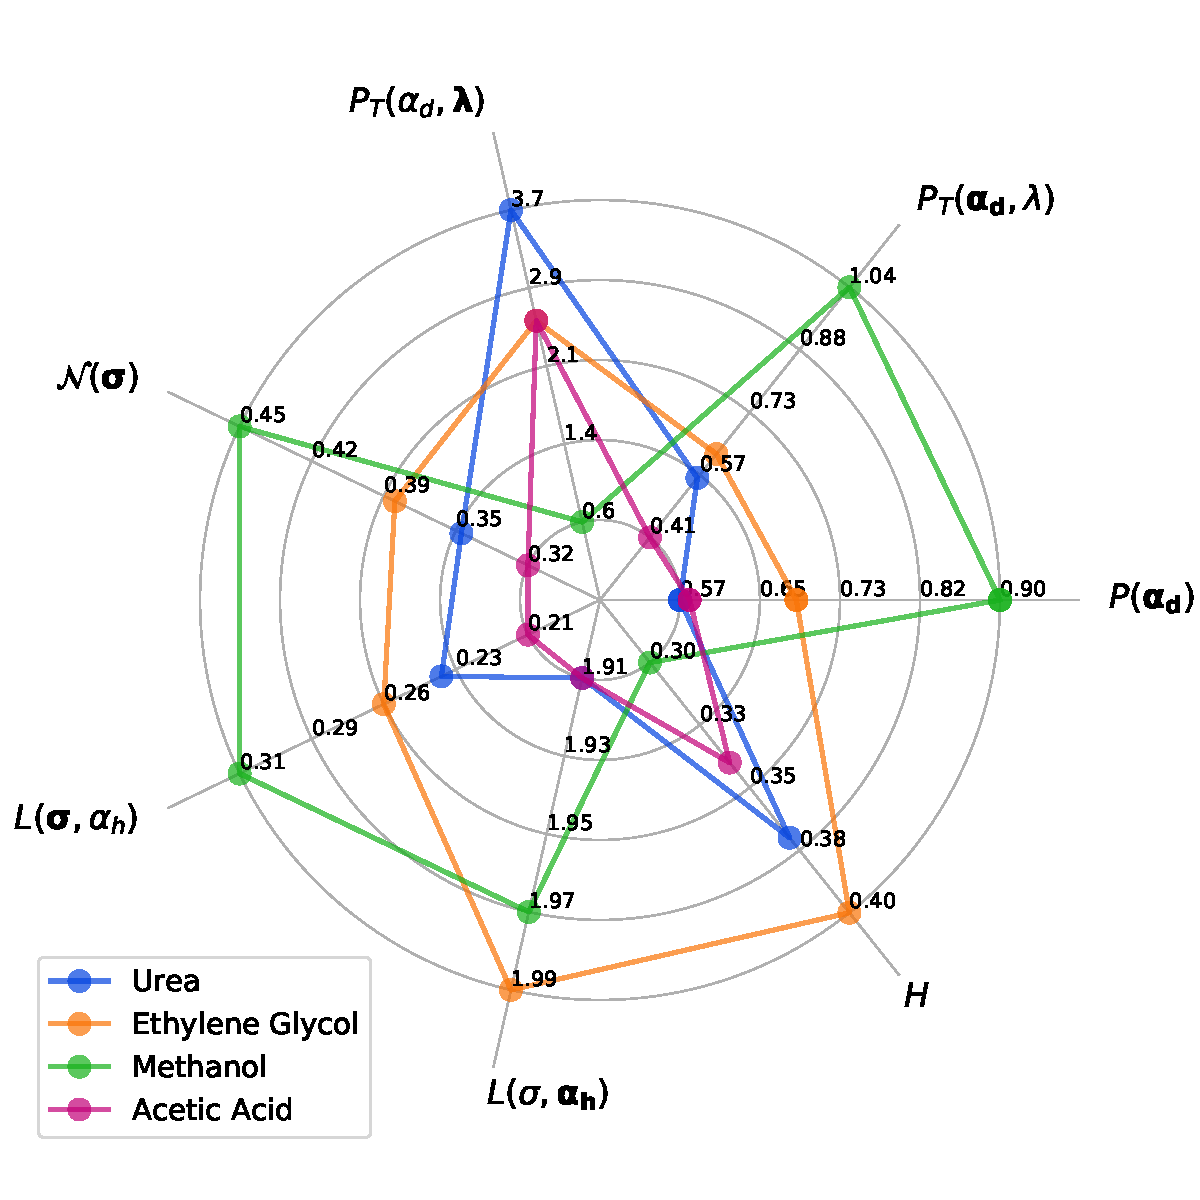
\includegraphics[width=\linewidth]{1mode_radar.pdf}
%  \caption{}\label{fig:1mode_radar}
%  \end{subfigure}
%  \begin{subfigure}{0.45\textwidth}
%  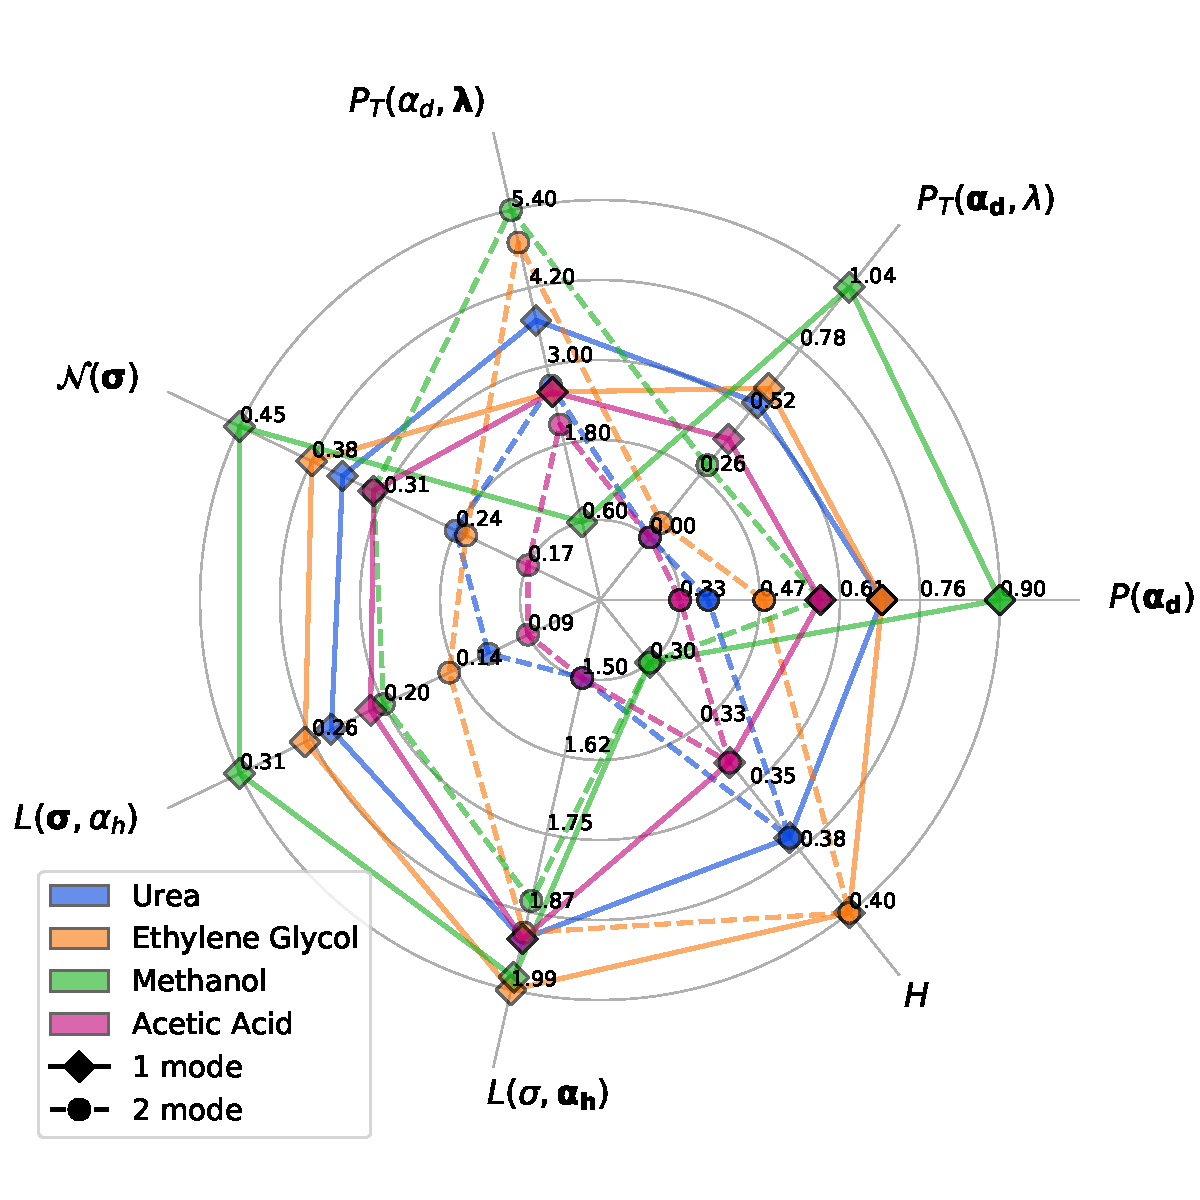
\includegraphics[width=\linewidth]{2mode_radar.pdf}
%  \caption{}\label{fig:2mode_radar}
%  \end{subfigure}
%  \caption{Another way to visualize Tables~\ref{table:sfbm_params} and~\ref{table:sfbm_params_2mode}}\label{fig:radars}
%  \end{figure}
%  
%  \begin{figure}
%  \centering
%  \begin{subfigure}{0.45\textwidth}
%  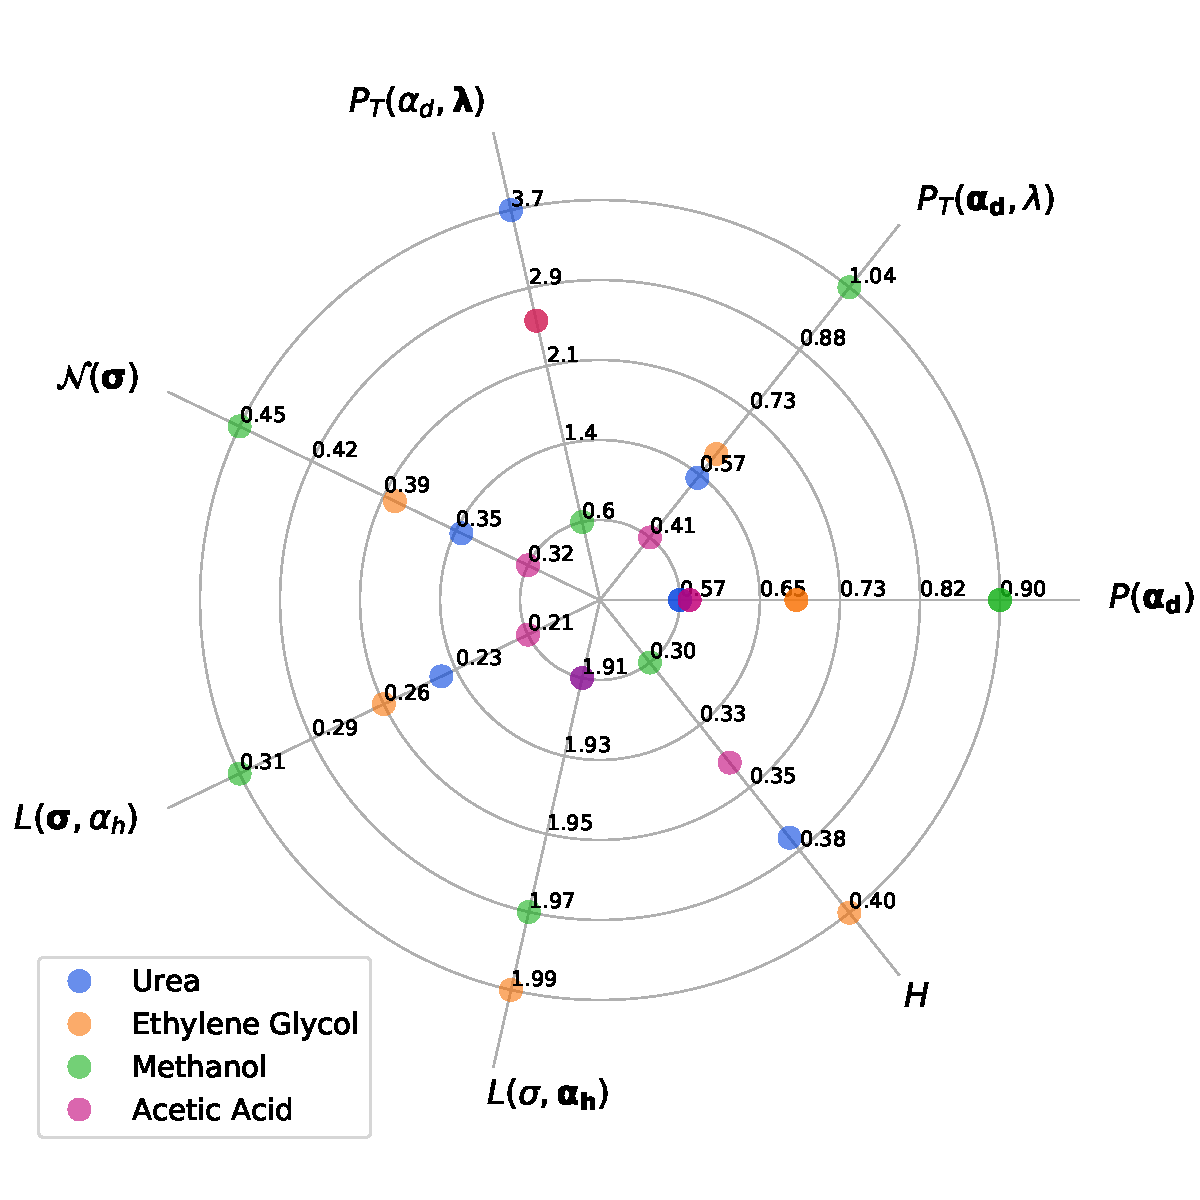
\includegraphics[width=\linewidth]{1mode_radar_nolines.pdf}
%  \caption{}\label{fig:1mode_radar}
%  \end{subfigure}
%  \begin{subfigure}{0.45\textwidth}
%  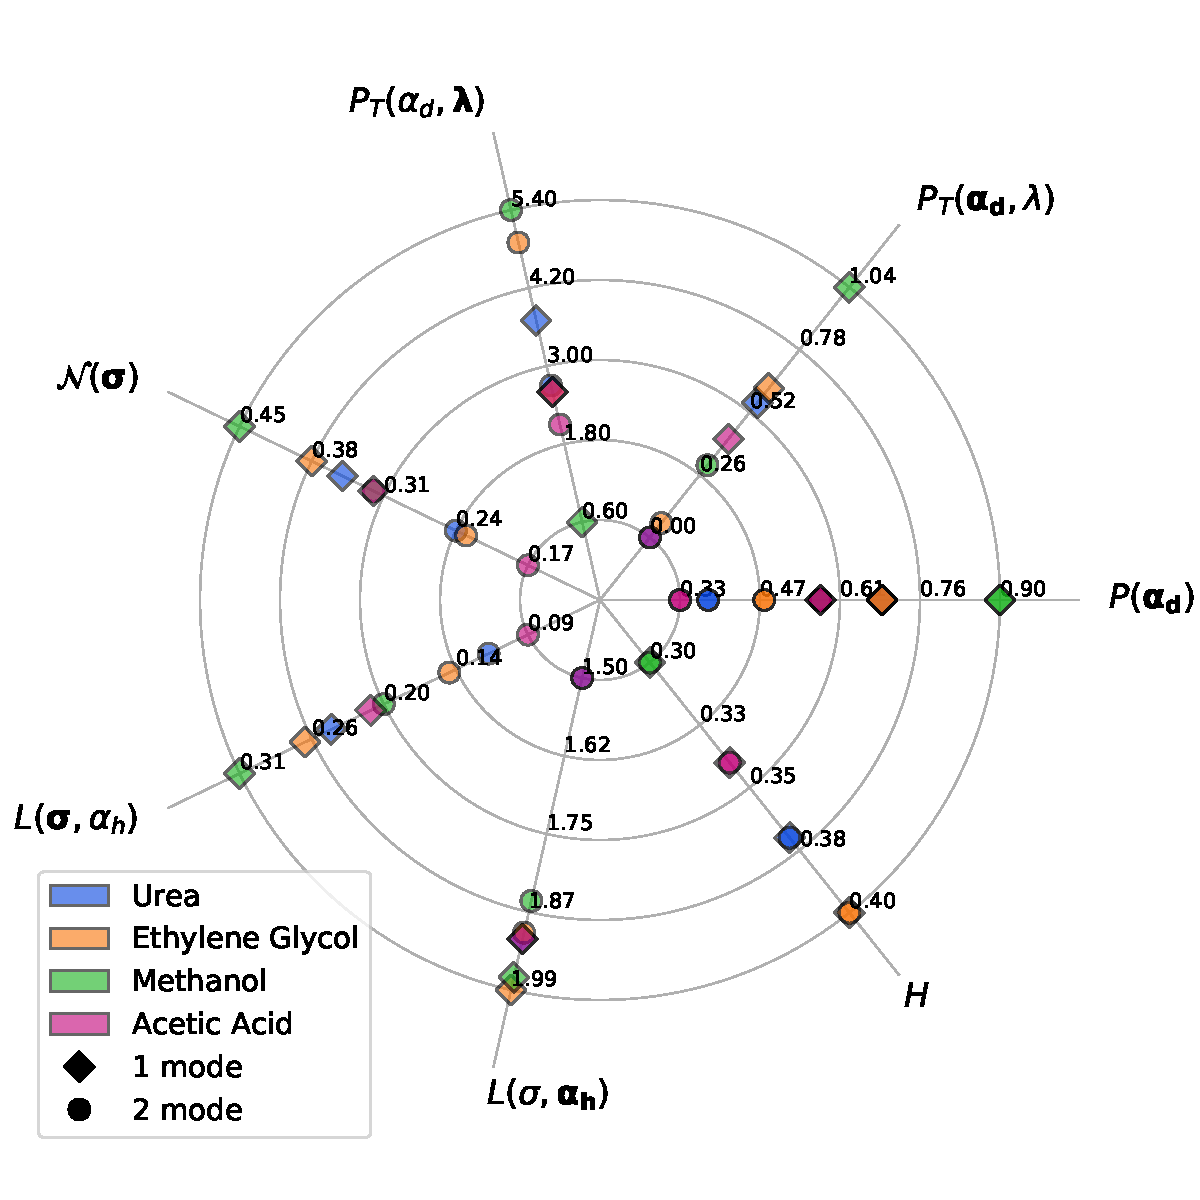
\includegraphics[width=\linewidth]{2mode_radar_nolines.png}   % for some reason it has trouble saving this as a PDF
%  \caption{}\label{fig:2mode_radar}
%  \end{subfigure}
%  \caption{Same as Figure~\ref{fig:radars} but with no lines between points}\label{fig:radars_nolines}
%  \end{figure}
  
%  \begin{figure}
%  \centering
%  \begin{subfigure}{0.45\textwidth}
%  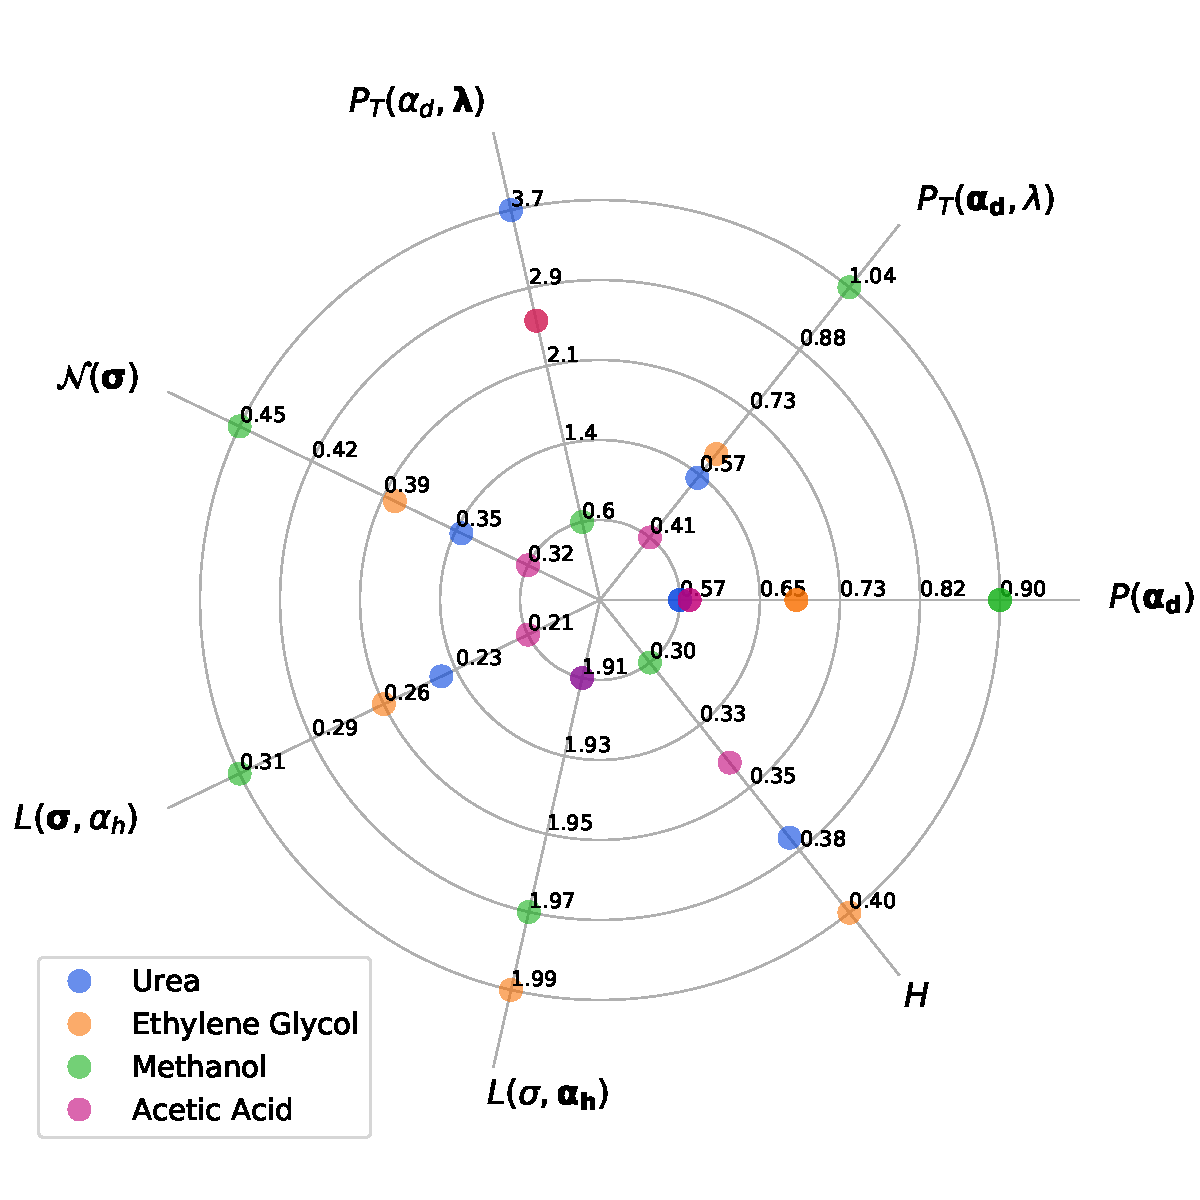
\includegraphics[width=\linewidth]{1mode_radar_nolines.pdf}
%  \caption{}\label{fig:1mode_radar_nolines}
%  \end{subfigure}
%  \begin{subfigure}{0.45\textwidth}
%  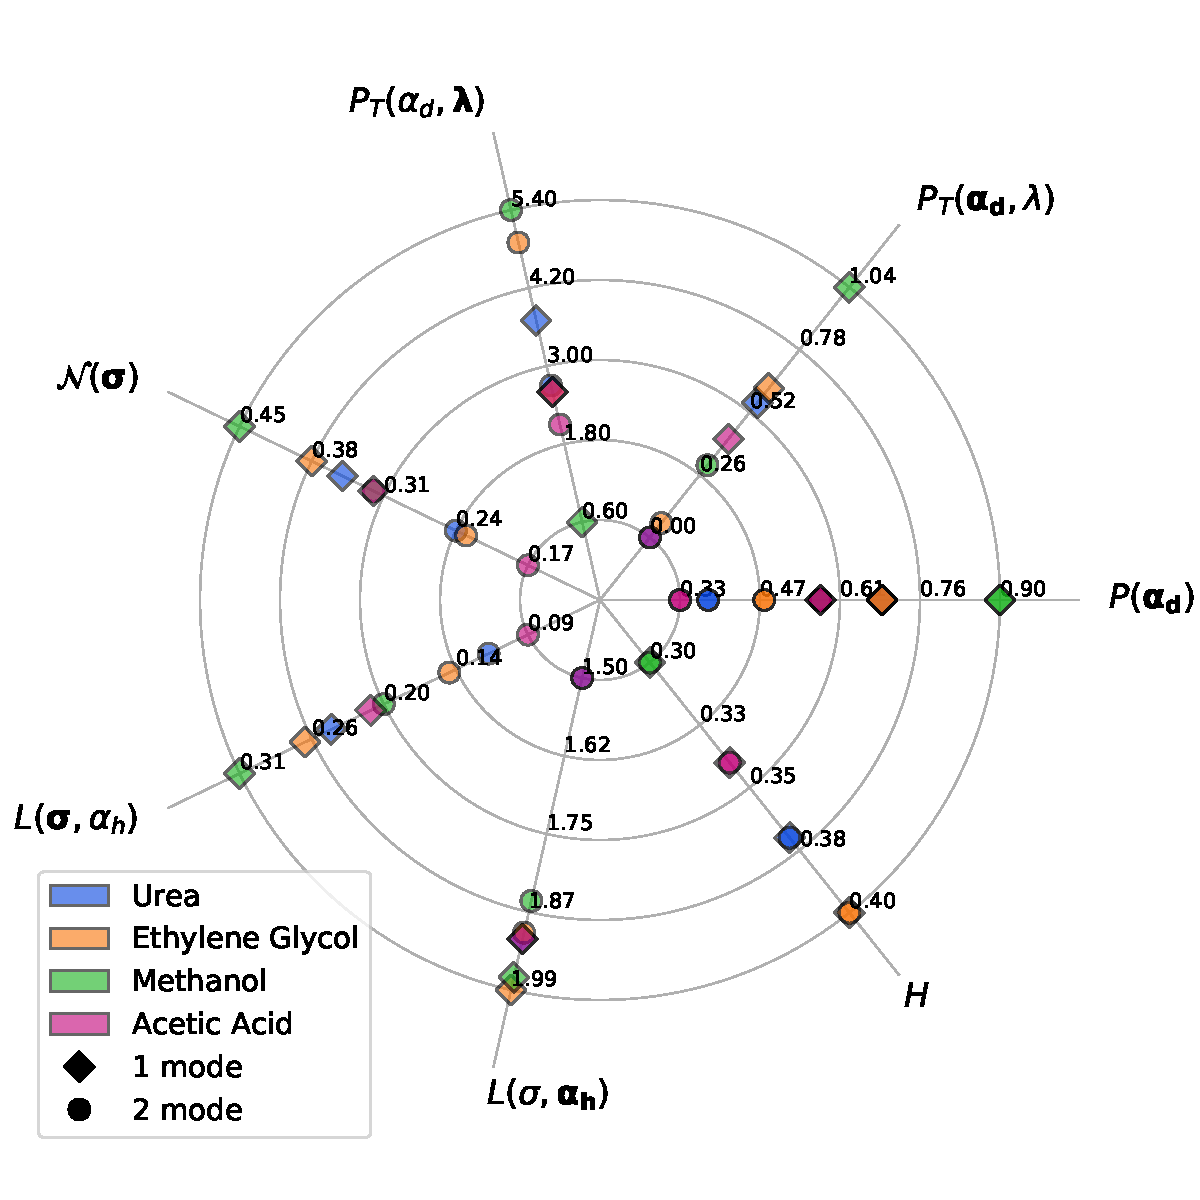
\includegraphics[width=\linewidth]{2mode_radar_nolines.pdf}
%  \caption{}\label{fig:2mode_radar_nolines}
%  \end{subfigure}
%  \caption{Same as Figure~\ref{fig:radars} but with no lines between points}\label{fig:radars_nolines}
%  \end{figure}
  
  Using the parameters in Tables~\ref{table:sfbm_params} and~\ref{table:sfbm_params_2mode}
  as inputs to our models, we obtain reasonable predictions of the MD simulated MSDs. The 
  MSD curves generated from 1 and 2 mode models are overlayed with the MD simulated MSDs for 
  comparison in Figures~\ref{fig:anomalous_msds_1mode} and~\ref{fig:anomalous_msds_2mode}
  respectively. 
  %The MSD of AD trajectories modeled using a power law with an exponential 
  %cut-off have a significantly reduced uncertainty and lie well within the error bars of MD.
  
  \begin{figure}
  \centering
  \begin{subfigure}{0.45\textwidth}
  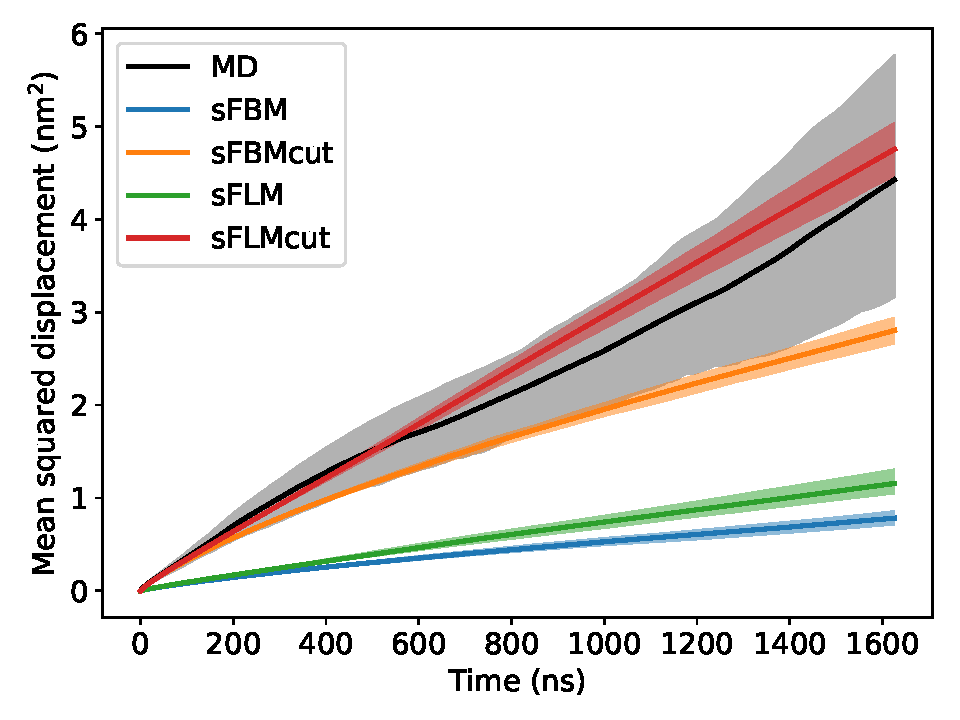
\includegraphics[width=\textwidth]{1mode_msd_comparison_URE.pdf}
  \caption{Urea}\label{fig:1mode_msd_comparison_URE}
  \end{subfigure}
  \begin{subfigure}{0.45\textwidth}
  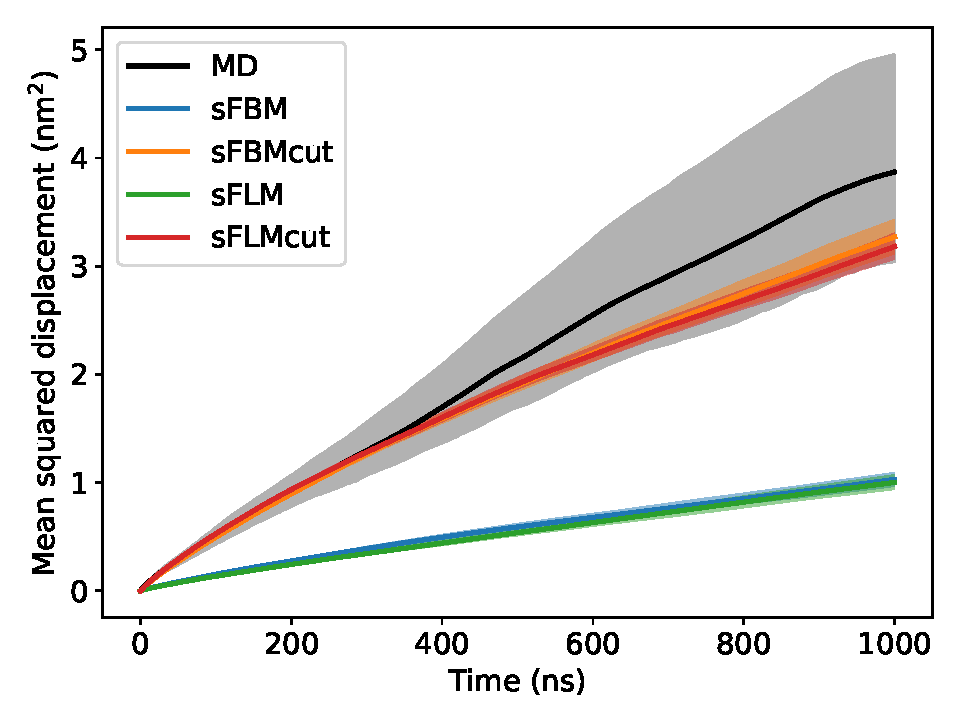
\includegraphics[width=\textwidth]{1mode_msd_comparison_GCL.pdf}
  \caption{Ethylene Glycol}\label{fig:1mode_msd_comparison_GCL}
  \end{subfigure}
  \begin{subfigure}{0.45\textwidth}
  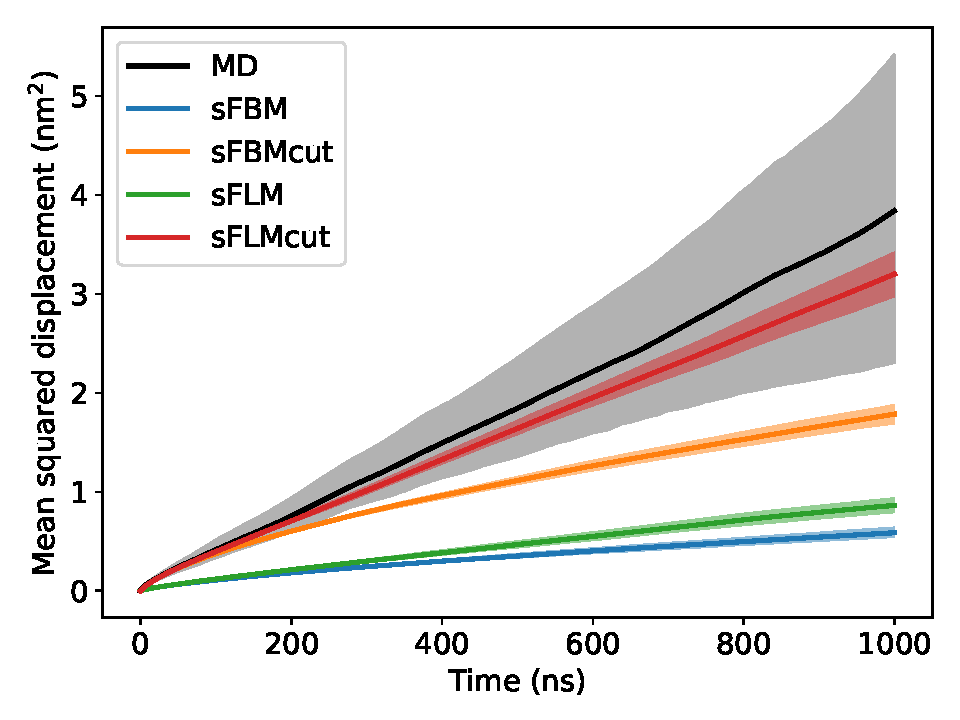
\includegraphics[width=\textwidth]{1mode_msd_comparison_MET.pdf}
  \caption{Methanol}\label{fig:1mode_msd_comparison_MET}
  \end{subfigure}
  \begin{subfigure}{0.45\textwidth}
  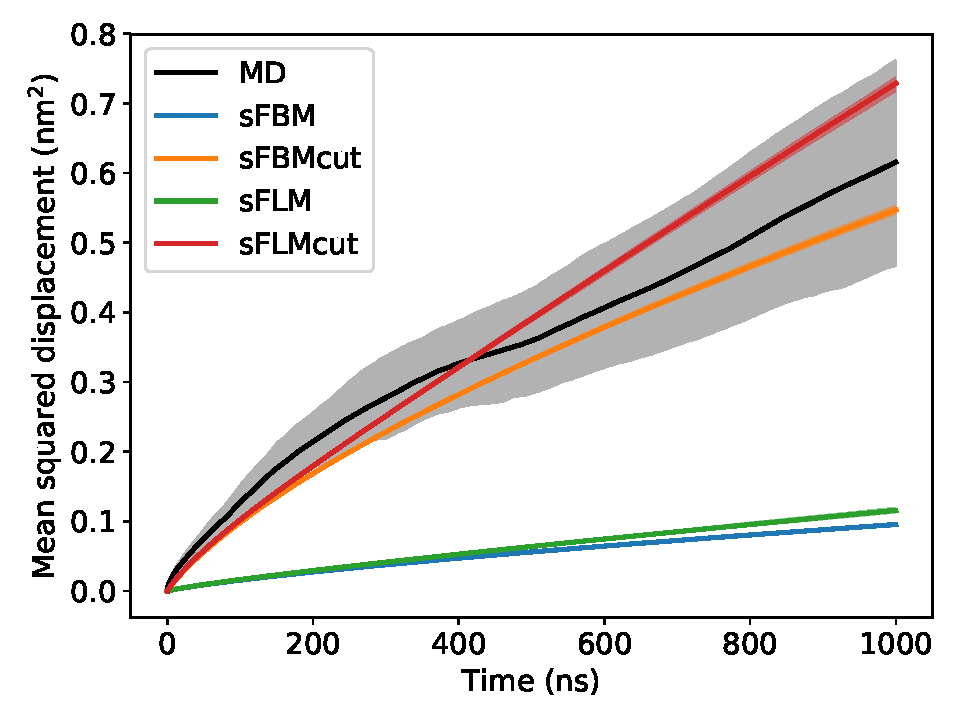
\includegraphics[width=\textwidth]{1mode_msd_comparison_ACH.pdf}
  \caption{Acetic Acid}\label{fig:1mode_msd_comparison_ACH}
  \end{subfigure}
  \caption{MSDs generated from realizations of our 1 mode anomalous diffusion models
  agree well with MD-generated data when using an exponential cutoff (sFBMcut and SFLMcut).
  When we do not apply an exponential cut-off to the dwell time distribution (sFBM 
  and SFLM), MSDs are underpredicted. Drawing hops from a truncated L\'evy stable 
  distribution results in higher MSDs than draws from Gaussians (sFLM and sFLMcut).}\label{fig:anomalous_msds_1mode}
  \end{figure}
  
  \begin{figure}
  \centering
  \begin{subfigure}{0.45\textwidth}
  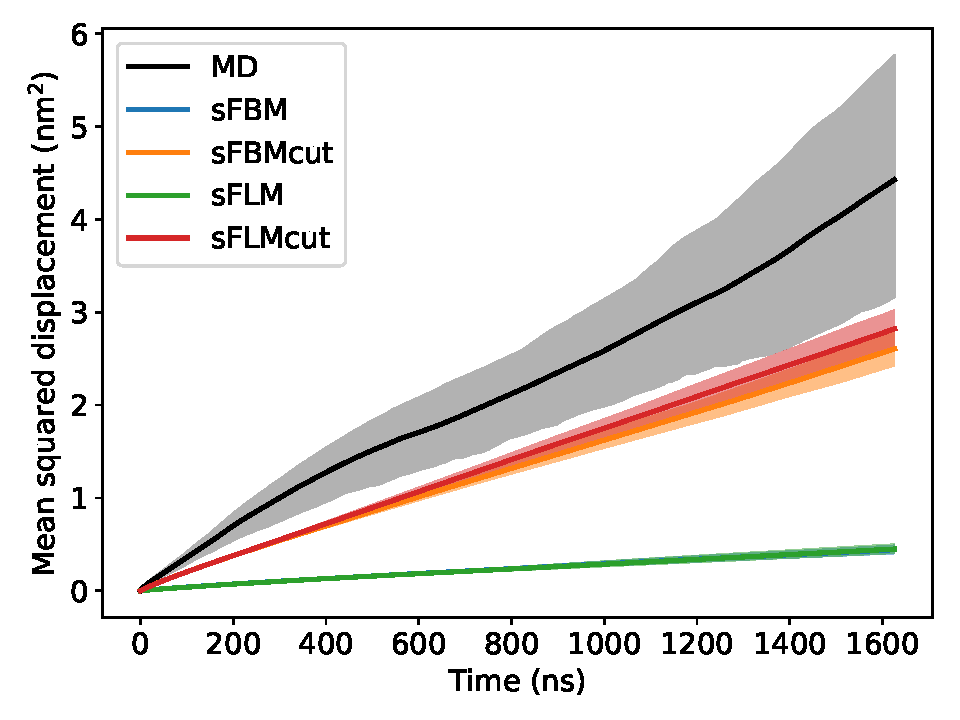
\includegraphics[width=\textwidth]{2mode_msd_comparison_URE.pdf}
  \caption{Urea}\label{fig:2mode_msd_comparison_URE}
  \end{subfigure}
  \begin{subfigure}{0.45\textwidth}
  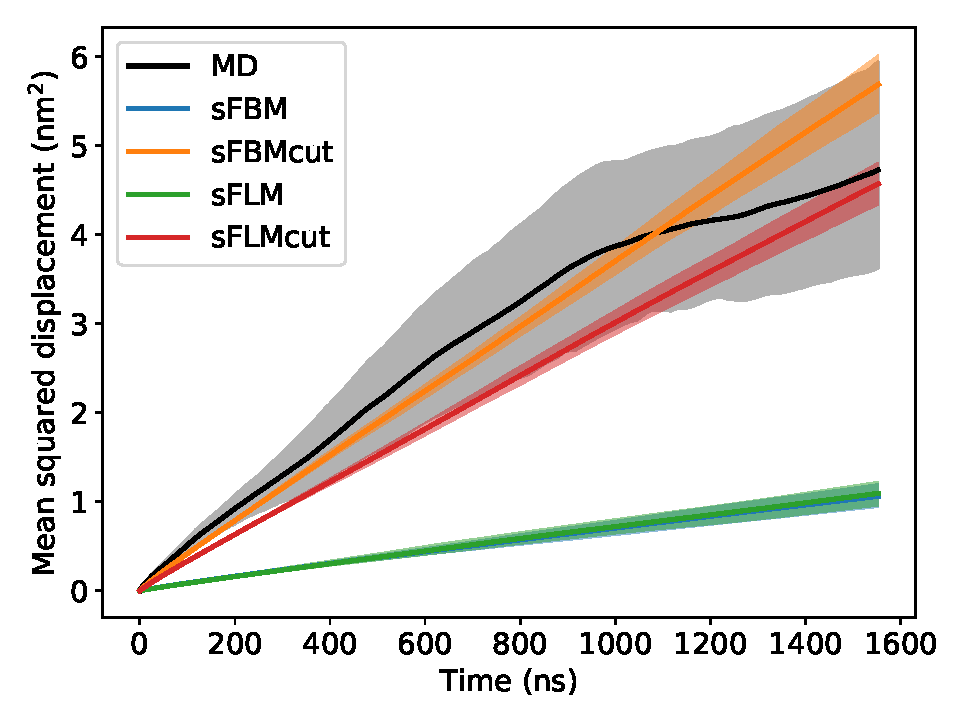
\includegraphics[width=\textwidth]{2mode_msd_comparison_GCL.pdf}
  \caption{Ethylene Glycol}\label{fig:2mode_msd_comparison_GCL}
  \end{subfigure}
  \begin{subfigure}{0.45\textwidth}
  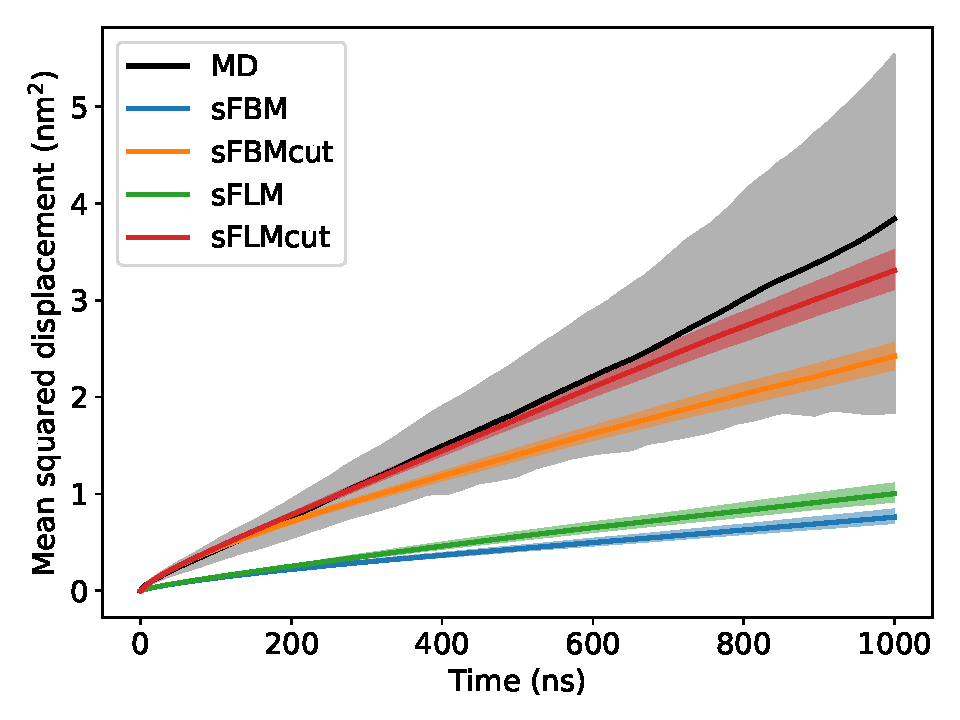
\includegraphics[width=\textwidth]{2mode_msd_comparison_MET.pdf}
  \caption{Methanol}\label{fig:2mode_msd_comparison_MET}
  \end{subfigure}
  \begin{subfigure}{0.45\textwidth}
  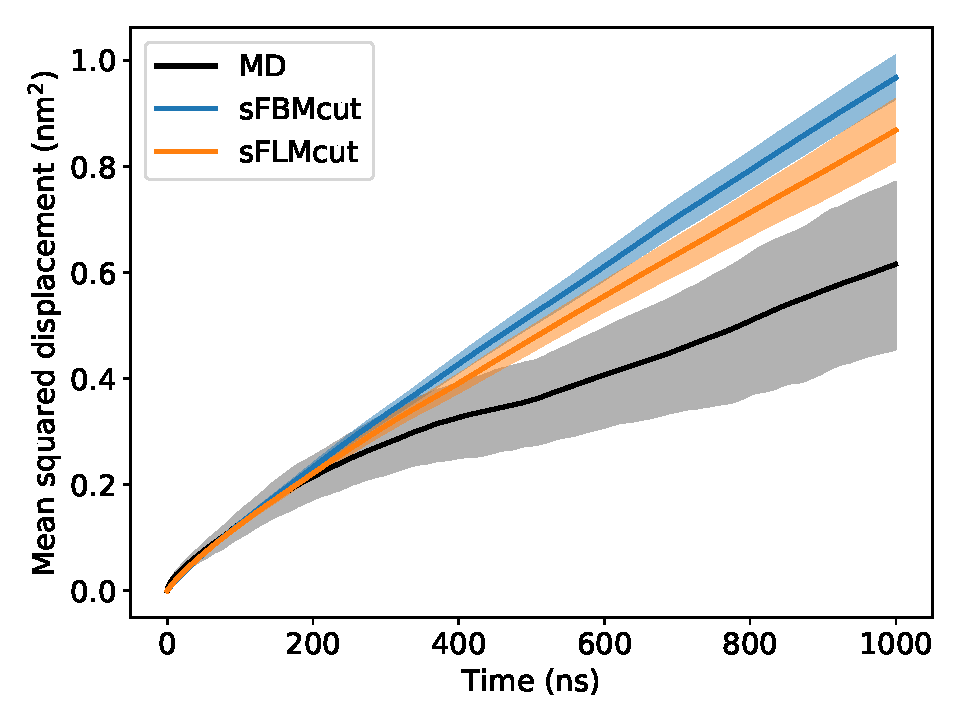
\includegraphics[width=\textwidth]{2mode_msd_comparison_ACH.pdf}
  \caption{Acetic Acid}\label{fig:2mode_msd_comparison_ACH}
  \end{subfigure}
  \caption{MSDs generated from realization of our 2-mode anomalous diffusion model
  also match well to MD-generated data. The MSD of urea appears to be underpredicted
  by all model combinations. The MSD of ethylene glycol is predicted well when 
  we draw dwell times from a power law distribution with an exponential cut-off.}\label{fig:anomalous_msds_2mode}
  \end{figure}
  
  Truncating the power laws with an exponential cut-off has the largest effect on the on 
  the match between the MD-calculated MSD and that measured from the simulated anomalous
  diffusion trajectories. Without truncation, the MD MSDs are underestimated in all cases.
  This is because dwell times on the order of the MD simulation length are sampled and 
  incorporated into the simulated anomalous diffusion trajectories, reducing the MSD. 
  The longest observed dwell time among the solutes was 1.3 $\mu$s by ethylene glycol.
  
  Simulated AD trajectories which draw from a L\'evy stable distribution generally 
  predict higher MSDs. The heavy tails of the distribution incorporate large
  jumps more frequently into the trajectories. The only exception is that of ethylene
  glycol in the 2 mode model where the L\'evy index for both modes is near 2, indicating
  a near Gaussian distribution.
  % BJC4: need to explain this somehow. 
  
  The model parameters for the 1 and 2 mode models tell stories about each solute's
  behavior that help explain the difference between the MSDs of different solutes. 
  Higher values of $\sigma$ and lower values of $\alpha_h$ indicate larger average 
  hop length magnitudes by increasing the hop length distribution's width and tail 
  density respectively. Higher values of $\alpha_d$ indicate a lower probability of 
  long dwell times. Higher values of $\lambda$ truncate the power law distribution 
  earlier preventing extremely long dwell times. Values of $H$ closer to the Brownian
  limit of 0.5, indicate a lower degree of negative correlation between hops. All 
  of which contribute to an overall increase in the MSD.
  
  Turning first to the parameters of the 1 mode model, we can begin to break down the
  trends in solute MSDs. The parameters belonging to ethylene glycol and methanol are
  relatively similar which is consistent with their similar MD-measured MSDs. Methanol 
  tends to stay trapped for less time and takes larger hops but the most substantial
  difference is with respect to their Hurst parameters. In fact, methanol has the lowest
  $H$ of all the solutes studied. It is possible that we have underestimated $H$ since 
  it appears that our model consistently under-predicts the methanol MSD curve relative
  to other solutes. However, it remains plausible that methanol does have a low $H$ 
  value because it spends the majority of its time outside the pore region where collisions
  with tails are frequent. Urea has the third highest MSD that is primarily a consequence of
  more frequent and long dwell times, indicated by lower values of $\alpha_d$ and 
  $\lambda$. Urea's hop lengths ($\sigma$) and correlation ($H$) are comparable to ethylene
  glycol and methanol. Acetic acid has the smallest MSD among the solutes studied due 
  to longer periods of entrapment and shorter hops. Its trapping behavior is parameterized
  by an $\alpha_d$ value significantly lower than other solutes, but an intermediate 
  $\lambda$ value, suggesting it experiences many medium length periods of entrapment. 
  Its hops are smaller but are slightly compensated by a heavier tailed distribution 
  (lower $\alpha_h$) than the other solutes. 
  
  We can use the 2 mode model to gain an even deeper understanding of solute behavior
  in the pore versus in the tails. It is clear that solutes are significantly slowed 
  while they are in the tail region (mode 2) where long dwell times are more probable
  (smaller $\alpha_d$) and hops are smaller (smaller $\sigma$). Interestingly, 
  $\alpha_h$ for urea and acetic acid in the tails is 1.50 meaning its hop distribution
  is heavy tailed relative to ethylene glycol and methanol whose $\alpha_h$ values are
  more consistent with a Gaussian distribution ($\alpha$=2). Acetic acid and urea are
  structurally similar molecules, both planar with two heavy atoms attached to a 
  carbonyl group. Their small size and rigid shape may allow them to occasionally slip
  through gaps in the tails. Meanwhile, methanol is small enough that it does not need
  to make larger jumps to escape traps. 
  
%  The parameters of the 1 mode model indicate some diversity in solute behavior. The value
%  of $\alpha_d$ for pure and truncated power law fits to the dwell time distributions of 
%  urea, ethylene glycol and methanol are similar. The value of $\alpha_d$ for acetic
%  acid is significantly lower than the rest of the solutes meaning it stays trapped 
%  for long periods of time more frequently. The value of $\lambda$ is largest for
%  methanol indicating that its longest dwell time is shorter than the longest dwell
%  times of all other solutes. When hops are fit to a Gaussian, it is clear that acetic
%  acid takes the smallest hops while methanol takes the largest. If we fit hops to a
%  L\'{e}vy stable distribution, we observe a similar trend in $\sigma$ values, but 
%  with varying weights on the distribution's tails. Acetic acid has the heaviest
%  tails (lowest $\alpha_h$), meaning it is more likely to take large hops, while 
%  ethylene glycol stays close to a Gaussian distribution (i.e. $\alpha_h$ near 2).
%  The Hurst parameters indicate a moderate degree of anti-correlation between hops. 
%  Surprisingly, methanol takes the most anti-correlated hops (lowest $H$). This is
%  likely because methanol spends the largest fraction of its time within the pores. 
%  It can still make large hops thanks to its small size, but tends to bounce around
%  the tails.

%  BJC4: urea and ethylene glycol only
%  The parameters of the 1 mode model are similar between urea and ethylene glycol which 
%  is not surprising considering their similar MD MSDs. Dwell times by 
%  ethylene glycol are shorter as shown by its larger $\alpha_d$ and $\lambda$ values. Both
%  solutes make similarly sized hops with hop distributions that are relatively close 
%  to Gaussian (i.e. $\alpha_h$ near 2) when fit to a L\'evy stable distribution. Finally,
%  both solutes exhibit a similar degree of correlation between hops with ethylene glycol
%  exhibiting motion closer to Brownian. 
  
%  The difference in parameters of each mode of the 2 mode sFBM model offer additional
%  mechanistic insight which the 1 mode model lacks. It is clear that solutes are 
%  significantly slowed while they are in the tail region (mode 2) where long dwell times
%  are more probable and hops are smaller (smaller $\alpha_d$). 
% BJC: I'm not sure how valid it is to analyze lambda because it is dependent on alpha. There is some counterbalancing going on.  
% The values of $\lambda$, however, do not 
% appear to be directly correlated to mode. For example, $\lambda$ for ethylene glycol is
% lower in the pores, meaning its longest dwell times in the pores are longer than its
% longest dwell times in the tails. This may be a consequence of    
%  Interestingly, $\alpha_h$ for urea and acetic acid in mode 2 is 1.50 meaning its 
%  hop distribution is heavy tailed relative to ethylene glycol and methanol whose 
%  $\alpha_h$ values are more consistent with a Gaussian distribution. Acetic acid and
%  urea are structurally similar molecules, both planar with two heavy atoms attached to
%  a carbonyl group. Their small size and rigid shape may allow them to slip through 
%  gaps in the tails. Meanwhile, methanol is small enough that it does not need to make 
%  larger jumps to escape traps. 
  
%  BJC4: Urea and ethlyene glycol only
%  The parameters of the 2 mode model are again similar between urea and ethylene glycol, 
%  but the difference between parameters of each mode offer more detailed mechanistic
%  insight than the 1 mode model. It is clear that solutes are significantly slowed while
%  they are in the tail region where long dwell times are more probable (lower $\alpha_d$)
%  and hops are smaller (smaller $\sigma$).  
%  Interestingly, $\alpha_h$ for urea in mode 2 is 1.50 meaning its hop distribution is
%  heavy tailed relative to ethylene glycol which has an $\alpha_d$ more consistent 
%  with a Gaussian distribution. Although urea's $\sigma$ parameter is much smaller in 
%  the tails, it still has an appreciable probability of making large hops. This could 
%  be a consequence of urea's relatively small size and rigid shape compared to ethylene glycol.
  %Ethylene glycol is a linear chain that can
  %easily become entangled among the alkane tails while urea is planar with its four
  %heavy atoms bonded to a single central atom.
  
  \subsubsection{Model validation on stationary trajectories}\label{section:sfbm_validation}

  We evaluated the predictive capabilities of the AD modeling approach by training
  the model parameters on the first half of the equilibrated MD trajectory data
  then comparing the MSD calculated from AD model realizations to the MSD calculated
  from the second half of the equilibrated MD trajectory data. This metric is
  only meaningful if the ensemble of solute trajectories is stationary.
  
  We observe that in many cases, the distribution of solutes within the membrane
  evolves slowly with time. We defined the perceived equilibration time point 
  for each solute based on the time at which the number of solutes inside the
  pores and tails stabilized. Nonetheless, we observe evidence of non-stationary
  solute behavior after equilibration, on the $\mu$s timescale. In Table~\ref{table:stationarity},
  we compare the MSD of the solutes calculated using trajectory data from the 
  first and second halves of the equilibrated simulation time. Ethylene glycol 
  and methanol show considerable differences in their MSDs. Urea and acetic acid
  appear to demonstrate satisfactory stationarity on the 5 $\mu$s timescale. The
  shapes of their MSDs curves are also very similar (see Figure~\ref{S-fig:msd_comparison}
  of the Supporting Information).
  
  \begin{table}[h]
  \centering
  \begin{tabular}{|c|c|c|}
  \hline
  \multirow{2}{*}{Residue} & \multicolumn{2}{c|}{MSD}            \\\cline{2-3}
                           & First Half       & Second Half      \\\hline
  Urea                     & 0.31 (0.23, 0.40)& 0.35 (0.28, 0.43)\\\hline
  Ethylene Glycol          & 3.11 (2.06, 4.25)& 1.03 (0.76, 1.29)\\\hline
  Methanol                 & 2.24 (1.61, 2.92)& 1.06 (0.77, 1.39)\\\hline
  Acetic Acid              & 1.58 (1.11, 2.03)& 1.43 (1.10, 1.73)\\\hline
  
  \end{tabular}
  \caption{In order to be considered stationary, the MSD of the ensemble of solute trajectories
  should be the same independent of the portion of equilibrated trajectory that is
  analyzed. The MSD values in this table are averages taken after a 500 ns time lag, 
  calculated independently from the first and second halves of the equilibrated
  solute trajectories. Urea and acetic acid both appear to satisfy the stationarity
  criteria, while ethylene glycol and methanol show significantly smaller MSDs 
  when calculated from the second half of the equilibrated trajectories.}\label{table:stationarity}
  \end{table}
  
  The non-stationary behavior of ethylene glycol and methanol present themselves
  in different ways. On average, methanol molecules in the tails appear to be 
  drifting further away from the pore center with time. Methanol's small size 
  significantly increases the volume of accessible structural space. Ethylene 
  glycol appears to experience an increased incidence of long trapping times. 
  These problems probably cannot be addressed without more simulation time or 
  additional solute trajectories. 

  Using the approach described above, we validated our 1 and 2 mode models with
  urea and acetic acid, since their trajectories appear stationary. The 
  resultant MSD plots are shown in Figure~\ref{fig:train_test}. 
  
  \begin{figure}
  \centering
  \begin{subfigure}{0.45\textwidth}
  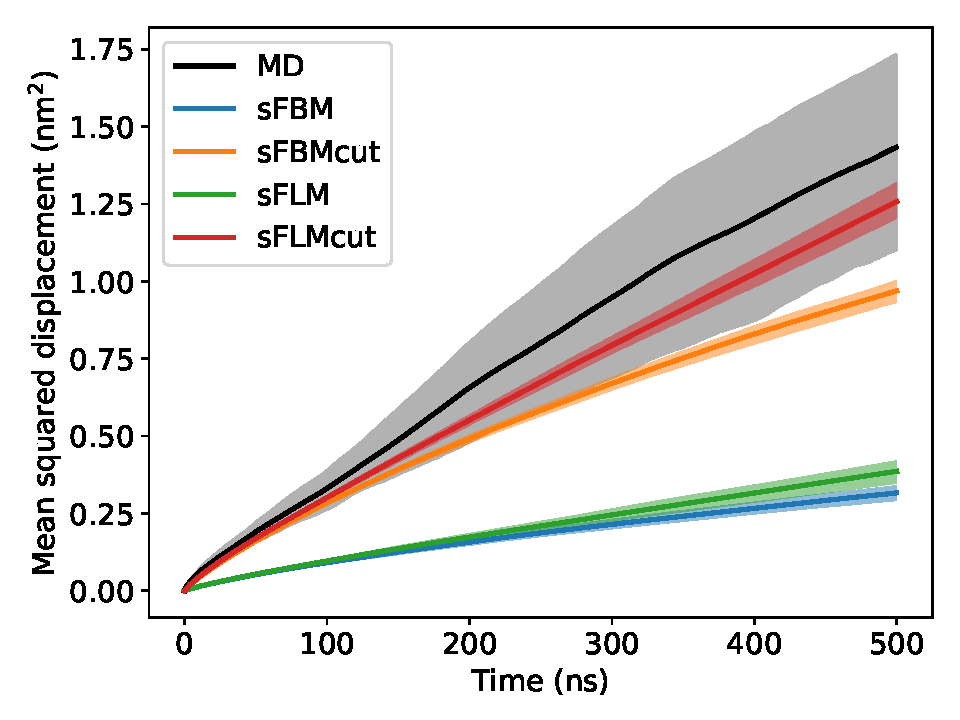
\includegraphics[width=\textwidth]{1mode_msd_comparison_URE_train_front.pdf}
  \caption{Urea (1 mode)}
  \end{subfigure}
  \begin{subfigure}{0.45\textwidth}
  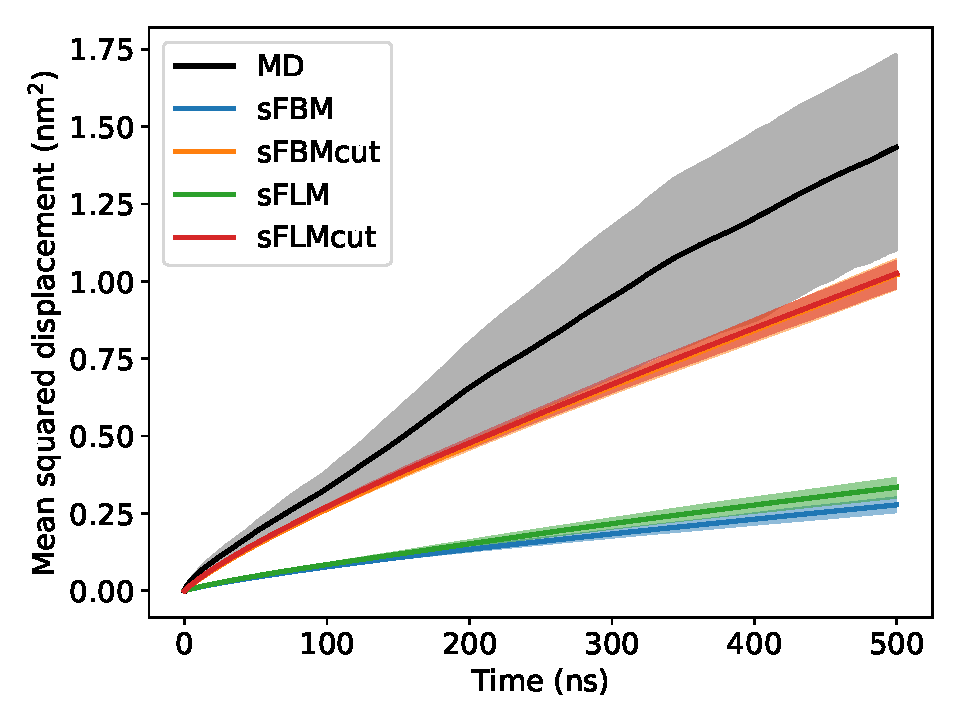
\includegraphics[width=\textwidth]{2mode_msd_comparison_URE_train_front.pdf}
  \caption{Urea (2 modes)}
  \end{subfigure}
  \begin{subfigure}{0.45\textwidth}
  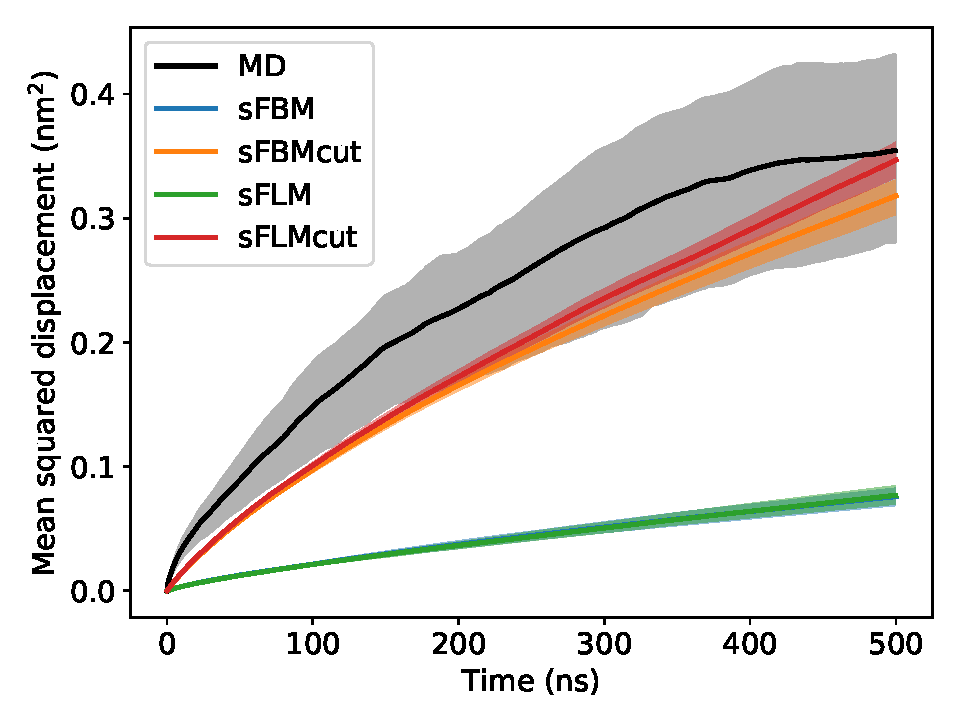
\includegraphics[width=\textwidth]{1mode_msd_comparison_ACH_train_front.pdf}
  \caption{Acetic acid (1 mode)}
  \end{subfigure}
  \begin{subfigure}{0.45\textwidth}
  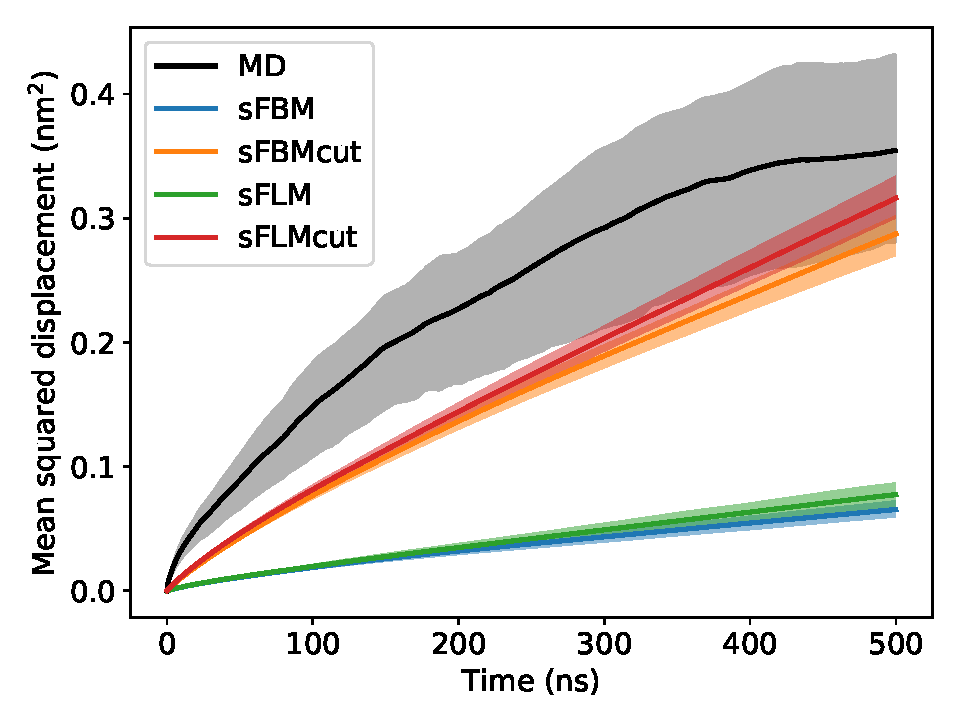
\includegraphics[width=\textwidth]{2mode_msd_comparison_ACH_train_front.pdf}
  \caption{Acetic acid (2 modes)}
  \end{subfigure} 
  \caption{The MSD curves predicted by the AD model trained on the first half 
  of the equilibrated data closely reproduce the MSD curves generated from the 
  second half of the equilibrated solute data.}\label{fig:train_test}
  \end{figure}
  
  The models reasonably predict the MSD of the second half of the solute 
  trajectories based on parameters generated from the first half. This success
  provides increased confidence in our ability to generate useful predictions
  of long time scale solute behavior
 
%  \begin{table}[h]
%  \centering
%  \begin{tabular}{|M{1.75cm}|M{1cm}|M{1.65cm}|M{2.5cm}|M{2.5cm}|M{2.5cm}|M{2.5cm}|}
%  \hline
%  \multirow{2}{*}{Solute}&\multirow{2}{*}{Modes}&\multirow{2}{*}{Model}&\multicolumn{2}{c|}{Trained on First Half} & \multicolumn{2}{c|}{Trained on Second Half}        \\\cline{4-7}
%                              &                   &        & MD MSD                & Prediction & MD MSD               & Prediction \\\hline
%  \multirow{4}{*}{Urea}       & \multirow{2}{*}{1}&sFBMcut&\multirow{4}{*}{1.43 (1.11, 1.76)}&0.31 (0.28, 0.35)&\multirow{4}{*}{1.43 (1.11, 1.77)}    &            \\\cline{3-3}\cline{5-5}\cline{7-7}
%                              &                   &sFLMcut&                         &0.35 (0.30, 0.40)&                     &            \\\cline{2-3}\cline{5-5}\cline{7-7}
%                              & \multirow{2}{*}{2}&sFBMcut&                         &0.23 (0.20, 0.27)&                     &            \\\cline{3-3}\cline{5-5}\cline{7-7}
%                              &                   &sFLMcut&                         &            &                     &            \\\hline
%                              & \multirow{2}{*}{1}&sFBMcut&\multirow{4}{*}{1.03 (0.79, 1.29)}        &            &\multirow{4}{*}{1.03 (0.77, 1.30)}    &            \\\cline{3-3}\cline{5-5}\cline{7-7}
%  Ethylene                    &                   &sFLMcut&                         &            &                     &            \\\cline{2-3}\cline{5-5}\cline{7-7}
%  Glycol                      &\multirow{2}{*}{2} &sFBMcut&                         &            &                     &            \\\cline{3-3}\cline{5-5}\cline{7-7}
%                              &                   &sFLMcut&                         &            &                     &            \\\hline
%  \multirow{4}{*}{Methanol}   &\multirow{2}{*}{1} &sFBMcut&\multirow{4}{*}{1.06 (0.69, 1.36)}        &            &\multirow{4}{*}{1.06 (0.67, 1.37)}    &            \\\cline{3-3}\cline{5-5}\cline{7-7}
%                              &                   &sFLMcut&                         &            &                     &            \\\cline{2-3}\cline{5-5}\cline{7-7}
%                              &\multirow{2}{*}{2} &sFBMcut&                         &            &                     &            \\\cline{3-3}\cline{5-5}\cline{7-7}
%                              &                   &sFLMcut&                         &            &                     &            \\\hline
%  \multirow{4}{*}{Acetic Acid}& \multirow{2}{*}{1}&sFBMcut&\multirow{4}{*}{0.35 (0.28, 0.45)}&0.31 (0.28, 0.35)&\multirow{4}{*}{0.35 (0.26, 0.47)}    &            \\\cline{3-3}\cline{5-5}\cline{7-7}
%                              &                   &sFLMcut&                         &0.35 (0.30, 0.40)&                     &            \\\cline{2-3}\cline{5-5}\cline{7-7}
%                              & \multirow{2}{*}{2}&sFBMcut&                         &0.23 (0.20, 0.27)&                     &            \\\cline{3-3}\cline{5-5}\cline{7-7}
%                              &                   &sFLMcut&                         &            &                     &            \\\hline
%  \end{tabular}
%  \caption{}\label{table:sFBM_train}
%  \end{table}
  
  %BJC3: Is it a bad idea to acknowledge that there is no experimental data? I can 
  % spin this paragraph in a different way.
  %MRS4: can one to training and validation?  Train on 1/2 the data, then see how well it fits the other half?
  %MRS4: also, you need to be more specific about choosing for WHAT purpose.  Different purposes could imply different models.
  Choosing which model to use for long timescale projections is not entirely obvious
  without experimental data to compare with. For our comparisons to MD, using a 
  truncated power law distribution is an obvious choice. However, given that extremely
  long dwells are a rare event, it is possible that studying a much larger set of 
  solutes will fill in the tail of the pure power law PDF. Regarding hop length 
  distributions, the generality of L\'evy stable distributions is powerful, but the
  lack of exact methods for simulation of fractional L\'evy motion reduces it's 
  accuracy and computational tractability. Treating the dynamics as fractional 
  Brownian motion is probably sufficient unless the L\'evy index, $\alpha_h$, is well below 2.
  
%  \noindent We can use the model to project our simulations out to very long timescales.
%  \begin{itemize}
%    \item We can not definitively say which combination of distributions are best to use.
%    \item Although the longest observed dwell times and hop lengths are less than
%    the length of the simulated trajectories and box lengths respectively, it is still possible
%    that that extremely long dwell times and hops are observed experimentally in rare but
%    significant cases.
%    \item We present long timescale projections using combinations of each distribution in the
%    table below
%  \end{itemize}

  % BJC2: table of long timescale projections using combinations of dwell and hop distributions. 
  %% TABLE %%

  \subsection{Markov State-Dependent Dynamics}\label{section:msm_results}
  
  %BJC4: maybe some kind of transitional paragraph here.  
  
  To create an MSDDM for each solute, we determined the state sequence of each 
  solute solute trajectory and then generated emission distributions for fluctuations
  within each state as well as transitions between states. There are not enough 
  consecutive observations of each type of transition with which to study their 
  individual correlation structures so we grouped all transition distributions
  into a single distribution and measured the correlation of the series of all 
  transitions. We lose information about individual types of transitions, however, 
  we believe this is unavoidable without at least an order of magnitude of additional data.
  
  We observe correlated emissions drawn from L\'evy stable distributions. The 
  deviation of the emission distributions from Gaussian behavior is far more pronounced
  than that seen in the hop length distributions of the previous section, therefore we 
  did not consider the Gaussian case (see Figure~\ref{fig:gaussian_levy_comparison}).
  The correlation structure between hops resembles that of FLM (Figure~\ref{fig:msddm_acf}).
  The parameters of the L\'evy stable distributions along with their Hurst parameters 
  are tabulated in Table~\ref{table:msddm_params}. 
  
  %MRS4: might this work better visually?  Table in SI, figure here?
  \begin{figure}
  \centering
  \begin{subfigure}{0.49\textwidth}
  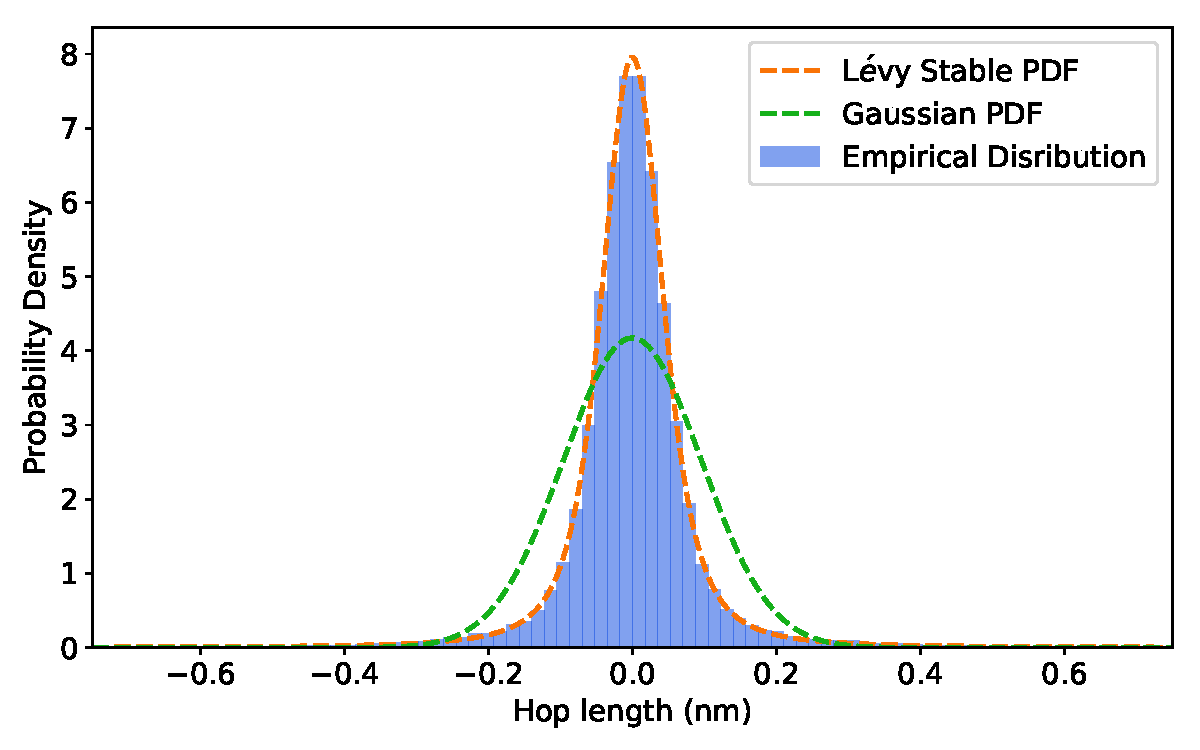
\includegraphics[width=\textwidth]{gaussian_levy_comparison.pdf}
  \caption{}\label{fig:gaussian_levy_comparison}
  \end{subfigure}
  % /figures/msddm_acf.py
  \begin{subfigure}{0.42\textwidth}
  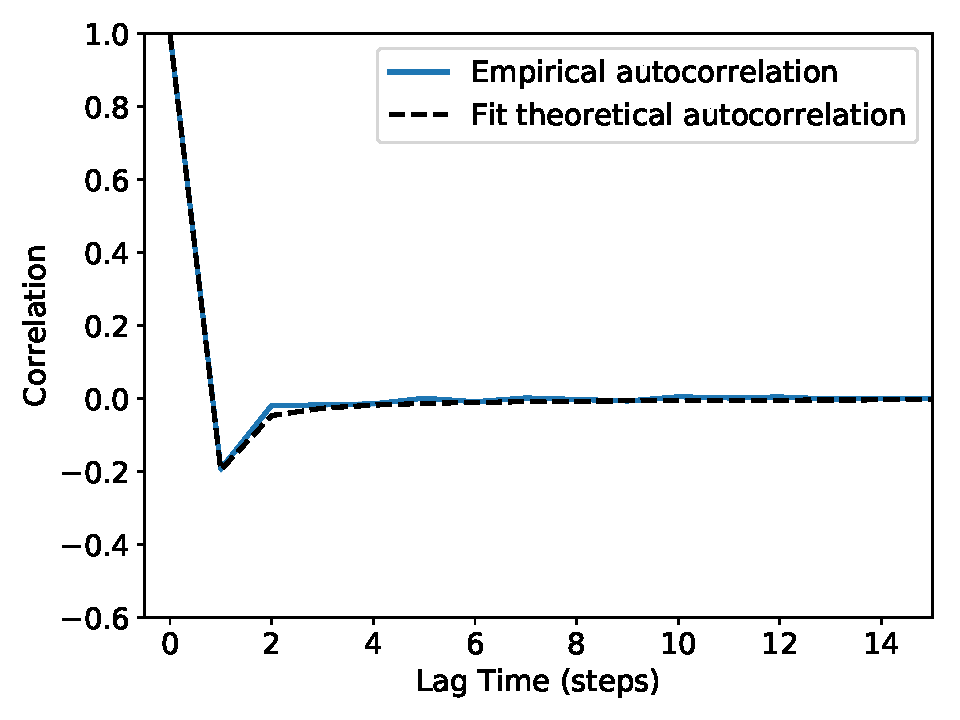
\includegraphics[width=\textwidth]{msddm_acf.pdf}
  \caption{}\label{fig:msddm_acf}
  \end{subfigure}
  \caption{(a) Emission distributions are non-Gaussian and heavy-tailed. Shown here is the
  emission distribution for transitions between states. The maximum likelihood
  Gaussian fit severely underestimates the empirical density of hops near and far from zero 
  while overestimating the density of hops at intermediate values. (b) Jumps drawn from
  the transition distribution are negatively correlated to each other. The normalized version 
  of Equation~\ref{eqn:flm_autocovariance} fits well to the data suggesting FLM is
  an appropriate way to model jumps.} \label{fig:msddm_emissions}
  \end{figure}
  
  \begin{table}[h]
  \centering
  \begin{tabular}{|c|c|c|c|c|c|c|c|c|c|c|c|c|}
  \hline
  & \multicolumn{3}{c|}{Urea} & \multicolumn{3}{c|}{Ethylene Glycol} & \multicolumn{3}{c|}{Methanol} & \multicolumn{3}{c|}{Acetic Acid} \\\hline
  State & H     &$\alpha_h$& $\sigma$ & H    &$\alpha_h$& $\sigma$   & H     &$\alpha_h$& $\sigma$ & H    &$\alpha_h$& $\sigma$ \\\hline
  1     & 0.10  & 1.79     & 0.034    & 0.09 & 1.68     & 0.045      & 0.11  & 1.56     & 0.052    & 0.10 & 1.78     & 0.035    \\
  2     & 0.06  & 1.80     & 0.033    & 0.09 & 1.75     & 0.037      & 0.07  & 1.63     & 0.043    & 0.08 & 1.88     & 0.032    \\
  3     & 0.11  & 1.88     & 0.030    & 0.11 & 1.86     & 0.030      & 0.02  & 1.80     & 0.036    & 0.04 & 2.00     & 0.030    \\
  4     & 0.10  & 1.95     & 0.027    & 0.04 & 1.91     & 0.028      & 0.02  & 1.75     & 0.036    & 0.04 & 2.00     & 0.027    \\
  5     & 0.19  & 1.34     & 0.048    & 0.15 & 1.40     & 0.062      & 0.10  & 1.28     & 0.074    & 0.13 & 1.47     & 0.048    \\
  6     & 0.15  & 1.45     & 0.040    & 0.11 & 1.52     & 0.040      & 0.03  & 1.50     & 0.042    & 0.09 & 1.70     & 0.038    \\
  7     & 0.15  & 1.61     & 0.032    & 0.05 & 1.60     & 0.040      & 0.28  & 1.20     & 0.043    & 0.08 & 1.77     & 0.031    \\
  8     & 0.11  & 1.71     & 0.028    & 0.05 & 1.74     & 0.030      & 0.04  & 1.83     & 0.037    & 0.01 & 2.00     & 0.030    \\
  T     & 0.34  & 1.42     & 0.036    & 0.37 & 1.44     & 0.045      & 0.35  & 1.45     & 0.057    & 0.34 & 1.54     & 0.040    \\\hline
  \end{tabular}
  \caption{We calculated values of $H$, $\alpha_h$ and $\sigma$ from MD simulation
  trajectories and used them to generate realizations of our MSDDM model. The states
  are defined in Table~\ref{table:states} except state T which describes the transition
  emissions.}\label{table:msddm_params}
  \end{table}
  
  
  %BJC4: better visualization scheme
  \begin{figure}
  \centering
  \begin{subfigure}{0.49\textwidth}
  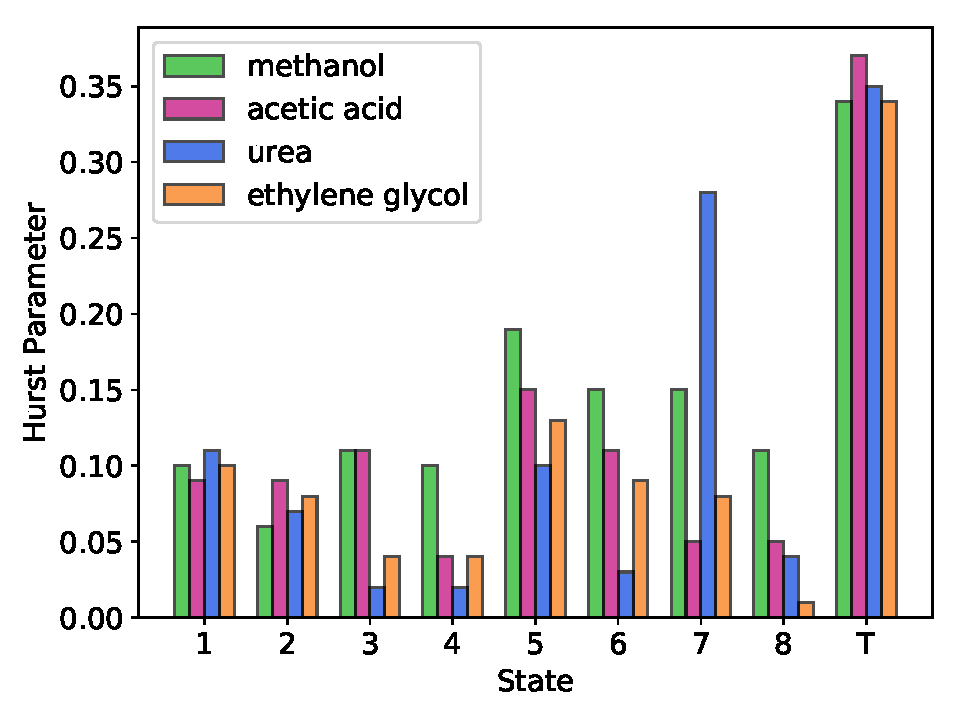
\includegraphics[width=\textwidth]{H_v_state.pdf}
  \caption{}\label{fig:H_v_state}
  \end{subfigure}
  \begin{subfigure}{0.49\textwidth}
  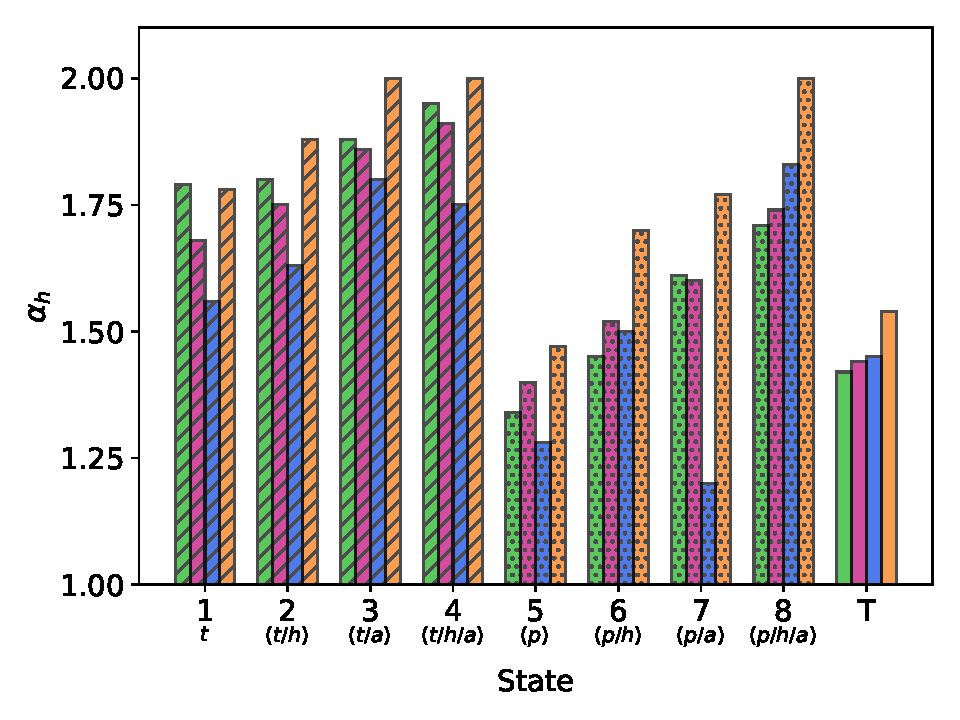
\includegraphics[width=\textwidth]{alpha_v_state.pdf}
  \caption{}\label{fig:alpha_v_state}
  \end{subfigure}
  \begin{subfigure}{0.49\textwidth}
  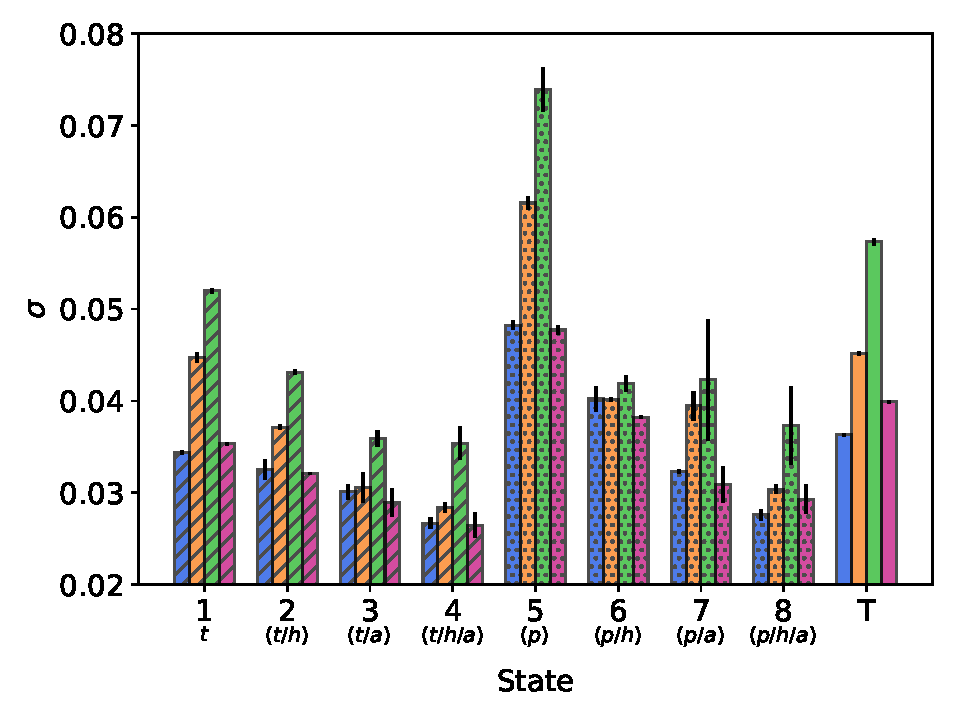
\includegraphics[width=\textwidth]{sigma_v_state.pdf}
  \caption{}\label{fig:sigma_v_state}
  \end{subfigure}
  \begin{subfigure}{0.49\textwidth}
  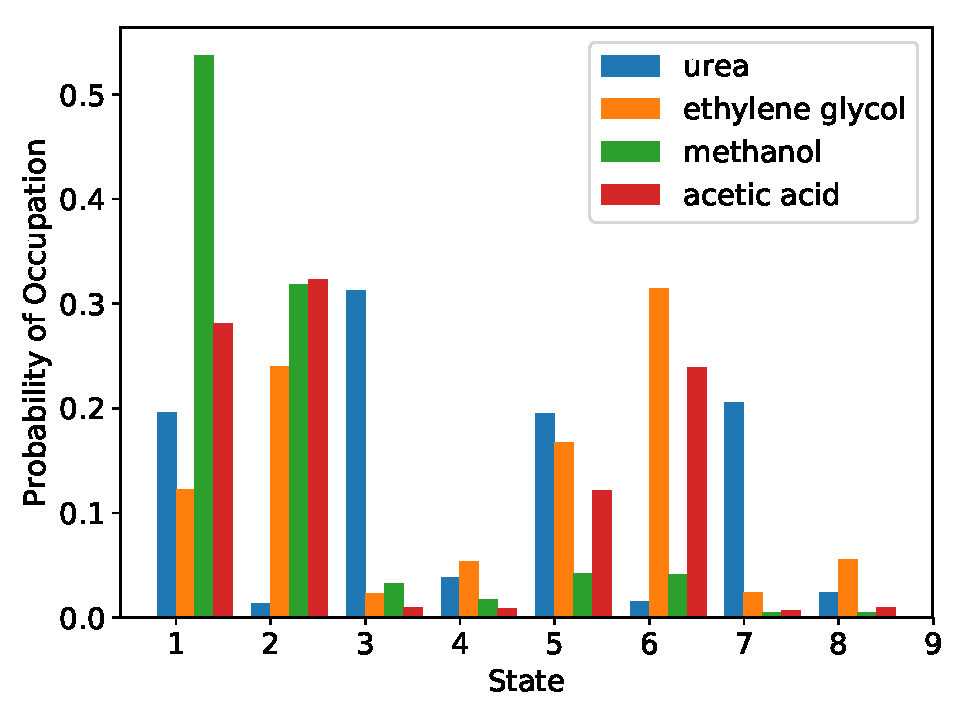
\includegraphics[width=\textwidth]{state_probabilities.pdf}
  \caption{}\label{fig:state_probabilities}
  \end{subfigure}
  \caption{We calculated values of $H$, $\alpha_h$ and $\sigma$ from MD simulation
  trajectories and used them to generate realizations of our MSDDM model. The states
  are defined in Table~\ref{table:states} except state T which describes the transition
  emissions.}\label{fig:msddm_parameters}
  \end{figure}
  
%  
%  \begin{table}[h]
%  \centering
%  \begin{tabular}{|c|c|c|c|c|c|c|c|c|}
%  \hline
%  & \multicolumn{4}{c|}{Urea}                      & \multicolumn{4}{c|}{Ethylene Glycol} \\\hline
%  State & H     & $\alpha_h$ & $\sigma$ & $T_{ii}$ & H    & $\alpha_h$ & $\sigma$ & $T_{ii}$  \\\hline
%  1     & 0.10  & 1.79       & 0.034    &  0.60    & 0.09 & 1.68       & 0.045    & 0.41 \\
%  2     & 0.06  & 1.80       & 0.033    &  0.38    & 0.09 & 1.75       & 0.037    & 0.58 \\
%  3     & 0.11  & 1.88       & 0.030    &  0.73    & 0.11 & 1.86       & 0.030    & 0.21 \\
%  4     & 0.10  & 1.95       & 0.027    &  0.57    & 0.04 & 1.91       & 0.028    & 0.34 \\
%  5     & 0.19  & 1.34       & 0.048    &  0.62    & 0.15 & 1.40       & 0.062    & 0.47 \\
%  6     & 0.15  & 1.45       & 0.040    &  0.38    & 0.11 & 1.52       & 0.040    & 0.62 \\
%  7     & 0.15  & 1.61       & 0.032    &  0.61    & 0.05 & 1.60       & 0.040    & 0.15 \\
%  8     & 0.11  & 1.71       & 0.028    &  0.41    & 0.05 & 1.74       & 0.030    & 0.29 \\
%  T     & 0.34  & 1.42       & 0.036    &   --     & 0.37 & 1.44       & 0.045    &  --  \\\hline
%  \end{tabular}
%  \caption{We calculated values of $H$, $\alpha_h$ and $\sigma$ from MD simulation
%  trajectories and then computed the average ensemble-averaged MSD of 10000 
%  simulated trajectories. The states are defined in Table~\ref{table:states}
%  except state T which refers to the transition emissions.}\label{table:msddm_params}
%  \end{table}
  
%  \begin{table}[h]
%  \centering
%  \begin{tabular}{|c|c|c|c|c|c|c|c|c|}
%  \hline
%  & \multicolumn{3}{c|}{Urea}                      & \multicolumn{3}{c|}{Ethylene Glycol} \\\hline
%  State & H     & $\alpha_h$ & $\sigma$  & H    & $\alpha_h$ & $\sigma$ \\\hline
%  1     & 0.10  & 1.79       & 0.034     & 0.09 & 1.68       & 0.045    \\
%  2     & 0.06  & 1.80       & 0.033     & 0.09 & 1.75       & 0.037    \\
%  3     & 0.11  & 1.88       & 0.030     & 0.11 & 1.86       & 0.030    \\
%  4     & 0.10  & 1.95       & 0.027     & 0.04 & 1.91       & 0.028    \\
%  5     & 0.19  & 1.34       & 0.048     & 0.15 & 1.40       & 0.062    \\
%  6     & 0.15  & 1.45       & 0.040     & 0.11 & 1.52       & 0.040    \\
%  7     & 0.15  & 1.61       & 0.032     & 0.05 & 1.60       & 0.040    \\
%  8     & 0.11  & 1.71       & 0.028     & 0.05 & 1.74       & 0.030    \\
%  T     & 0.34  & 1.42       & 0.036     & 0.37 & 1.44       & 0.045    \\\hline
%  \end{tabular}
%  \caption{We calculated values of $H$, $\alpha_h$ and $\sigma$ from MD simulation
%  trajectories and then computed the average ensemble-averaged MSD of 10000 
%  simulated trajectories. The states are defined in Table~\ref{table:states}
%  except state T which refers to the transition emissions.}\label{table:msddm_params}
%  \end{table}

  Most of a solute's MSD is a consequence of transitions between the 8 states
  in Table~\ref{table:states}. Motion while trapped in a state is highly 
  anti-correlated as indicated by their consistently low Hurst parameters.
  Perfectly anti-correlated motion ($H$=0) results in no contribution to the solute's
  MSD. Surprisingly, state 5 $H$ values are low despite the solutes being subject to no
  trapping mechanisms. Highly anti-correlated behavior in the pores in the absence of
  any trapping mechanism is likely caused by collisions with monomer head groups 
  within the pore region. The Hurst parameters for transitional (T) emissions are 2-18 times higher 
  than emissions from trapped states. The value of $\alpha_h$ for transition 
  emissions is also relatively low giving higher probabilities to larger hops.
  
  As solutes are influenced by more trapping effects simultaneously, the width of
  the hop length distribution, $\sigma$, decreases while its L\'evy index increases.
  Treating the tail and pore regions independently, $\sigma$ is largest and $\alpha_h$
  is smallest when solutes are not hydrogen bonding or associating with sodium (states 1 and 5).
  Solutes are free to move and take occasionally large hops. The smallest $\sigma$
  and highest $\alpha_h$ values are measured when solutes are hydrogen bonding and 
  associating with sodium at the same time (states 4 and 8). Motion is restricted 
  by multiple tethers which maintains a relatively narrow distribution of hop lengths.
  
  The trapping mechanisms affect each solute to varying degrees. The probabilities
  of occupying a given state at any time are plotted in Figure~\ref{fig:state_probabilities}.
  Urea and acetic acid spend slightly more than half their time in the tails (56\% and 62\% 
  of their time respectively) while ethylene glycol spends about 44\% of its time in the tails.
  Urea and acetic acid's compact and flat structure allows it to more easily 
  partition into the tails while ethylene glycol prefers the pore region due to 
  its two hydrophilic hydroxyl groups. Meanwhile methanol spends 91 \% of its 
  time in the tails likely due to its small size.
  
  %MRS4: make it more clear you are still taking about trapping mechanisms here.
  Urea spends the largest fraction of its time trapped via association with sodium ions.
  It does so 31\% of the total time while in the tails (state 3) and 21\% of the
  total time while in the pores (state 7). The electron-dense and unshielded oxygen
  atom of urea's carbonyl group is prone to associate with positively charged sodium
  ions. The nitrogen atoms of urea are only weak hydrogen bond donors.
  
  Ethylene glycol spends the largest fraction of its time trapped in a hydrogen
  bonded state. It does so 24\% of the total time while in the tails (state 2)
  and 32\% of the total time while in the pores (state 6). The two hydroxyl groups 
  of ethylene glycol readily donate their hydrogen atoms to the carboxylate
  head groups and the ether linkages between the head groups and monomer tails. 
  
  Methanol spends most of its time unbound in the tail region (state 1) and spends a 
  significant portion of time hydrogen bonded to while in the tail regions.
  Most of the tail region hydrogen bonds are donated from methanol to the ether
  linkages between the monomer head groups and tails.
  
  Finally, acetic acid spends the majority of it's time hydrogen bonding in and out
  of the pore.
  
  % /figures/msddm_state_probabilities.py
  %BJC4: combined with previous figure.
%  \begin{figure}
%  \centering
%  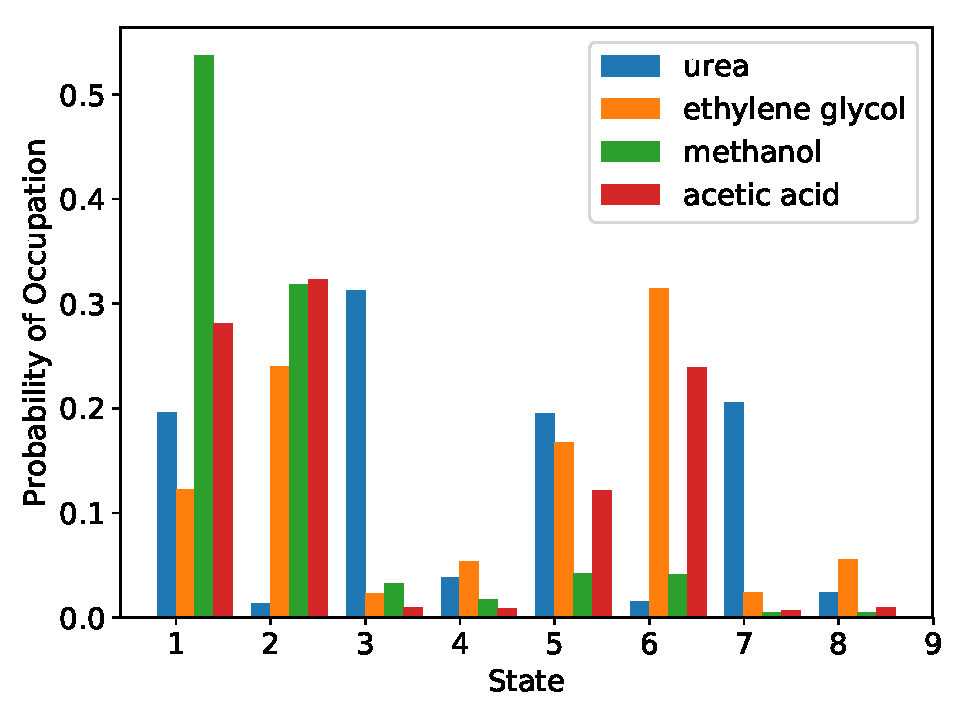
\includegraphics[width=0.5\textwidth]{state_probabilities.pdf}
%  \caption{The probability of finding urea or ethylene glycol in a given state.}\label{fig:state_probabilities}
%  \end{figure}
%  
  
  %BJC3: show how much of the MSD comes from each? Not sure this will work because of transition matrix dependence
  %BJC3: can just say 
  
  % BJC2: This figure will show predicted MSDs versus MD MSDs
  \begin{figure}
  \centering
  \begin{subfigure}{0.45\textwidth}
  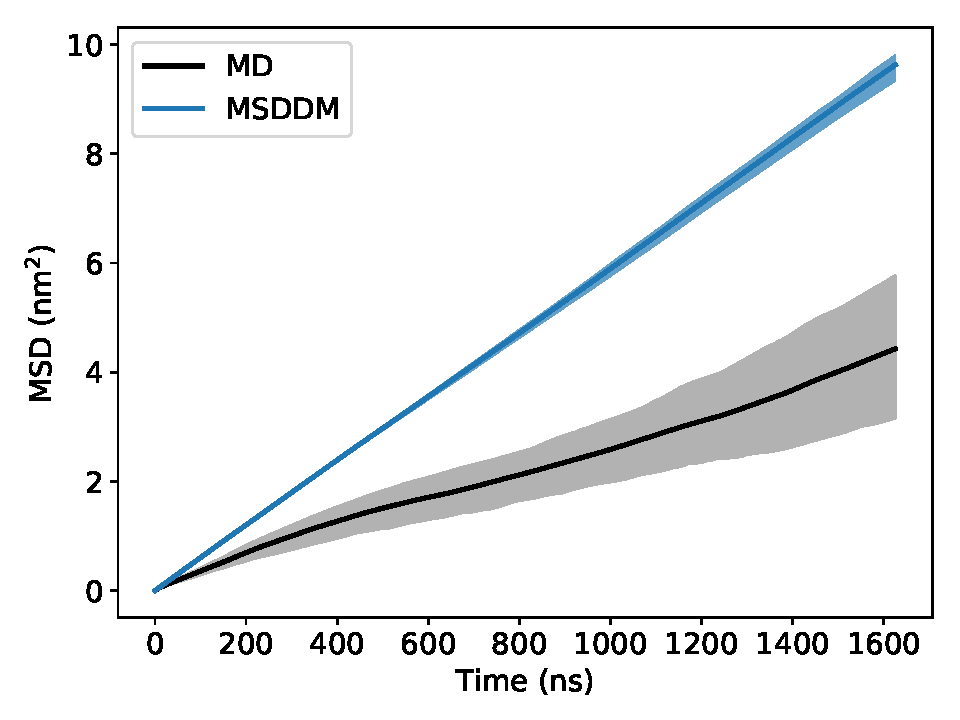
\includegraphics[width=\textwidth]{URE_msddm.pdf}
  \caption{}\label{fig:URE_msddm}
  \end{subfigure}
  \begin{subfigure}{0.45\textwidth}
  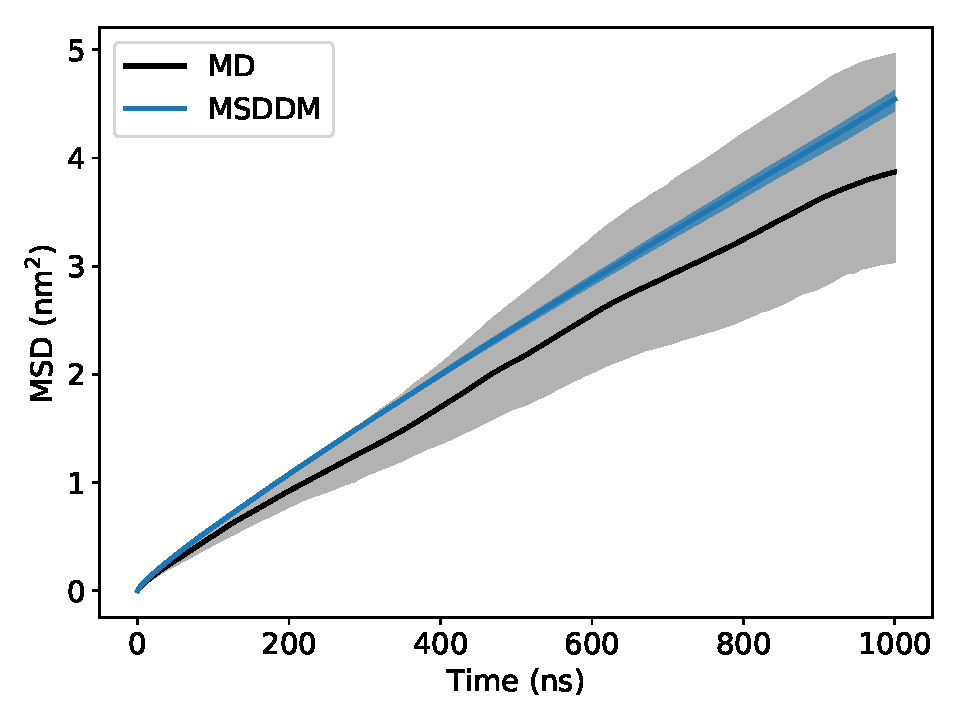
\includegraphics[width=\textwidth]{GCL_msddm.pdf}
  \caption{}\label{fig:GCL_msddm}
  \end{subfigure}
  \begin{subfigure}{0.45\textwidth}
  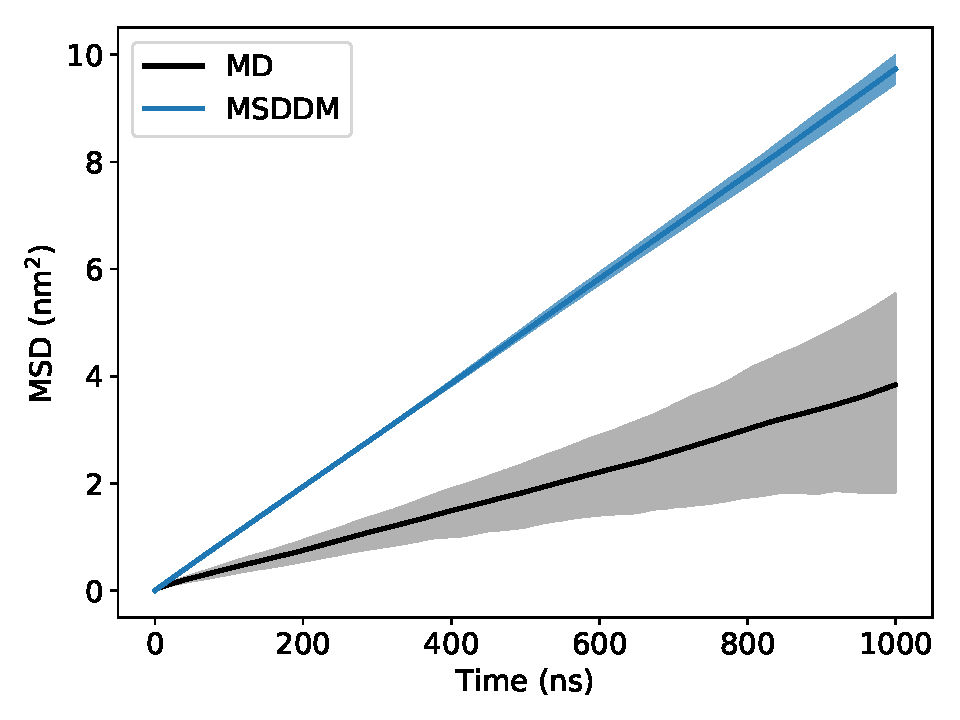
\includegraphics[width=\textwidth]{MET_msddm.pdf}
  \caption{}\label{fig:MET_msddm}
  \end{subfigure}
  \begin{subfigure}{0.45\textwidth}
  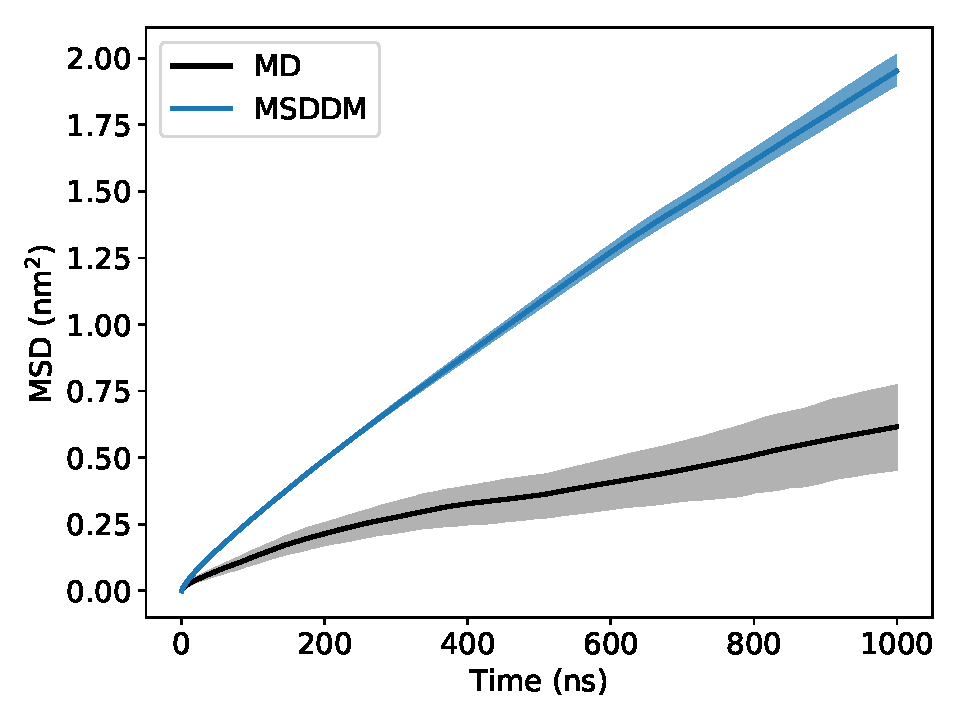
\includegraphics[width=\textwidth]{ACH_msddm.pdf}
  \caption{}\label{fig:ACH_msddm}
  \end{subfigure}
  \caption{MSDs predicted by the MSDDM significantly over-predict those
  from generated from MD simulations.}\label{fig:msddm_performance}
  \end{figure}
  
  %BJC3: would take ~ 20 hours to simulation 10000 trajectories.
  %MRS4: state how much it overestimated (1% or 10000%?)
  %BJC4: added percentages. Is it redundant since I already said how many time
  The MSDDM over-estimates solute MSDs by 200--300 \% (see Figure~\ref{fig:msddm_performance}). 
  We simulated 1000 trajectories as described in Section~\ref{method:MSMs} then
  %BJC3: 2.2 and 3.3 x higher than MD to be exact
  calculated their MSDs. The MSDs of urea and ethylene glycol are about 2 and 3 times
  higher than MD simulations respectively.
 
  %MRS4: It's not as clear what effect you are talking about until
  %later, i.e. the fact that the correlation is destroyed by the
  %state switching.
  %BJC4: modified thesis
  The MSDDM overestimates solute MSDs because correlation is lost
  every time a state switch occurs. Although correlation exists within each
  sequence, there is no memory of the previous state or state transition 
  that can be built into the first emission of the most recent state. 
  This implies that the first value in a state sequence is a random
  draw from the underlying emission distribution. Frequent transitions
  between states lead to an abundance of short dwell times. It is 
  difficult to accurately correlate short sequences so we are 
  almost simulating uncorrelated draws from the emission distribution.
  In Figure~\ref{fig:T_sensitivity}, we demonstrate this effect by varying 
  the transition matrix and simulating a simple 2-state model with parameters
  similar to those in Table~\ref{table:msddm_params} (see Table~\ref{S-table:msddm_params}
  of the Supporting Information). We modified the probability
  transition matrix, $T$, in order to control the probability of 
  self-transitions (the diagonal elements of $T$). Larger self-transition probabilities lead to longer dwell 
  times in each state. We set the off-diagonal elements of $T$ to be equal values that make the
  rows of $T$ sum to unity when combined with the self-transition probabilities. 
  As we increase the self-transition probability, $T_{ii}$, the simulated MSD 
  decreases. Consequently longer dwell times in each state allow us to more accurately
  simulate the negative correlation that we observe in MD.
  
  \begin{figure}
  \centering
  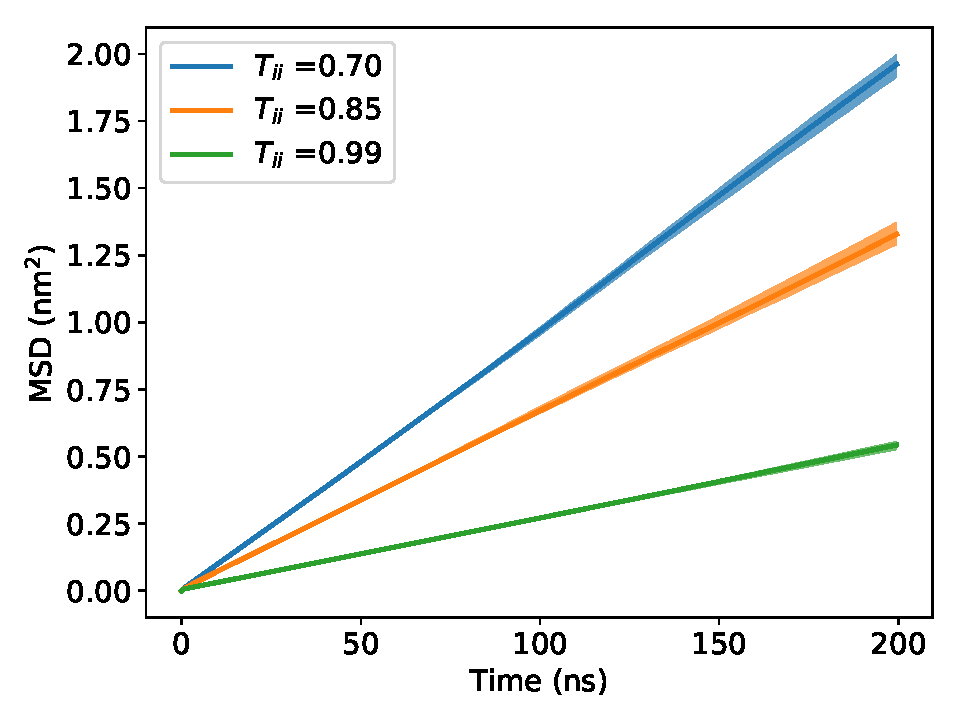
\includegraphics[width=0.5\textwidth]{T_sensitivity.pdf}
  \caption{As we increase the self-transition probabilities ($T_{ii}$) of an MSDDM,
  the simulated MSD of the process decreases because the negative correlation structure
  of individual state sequences is simulated more accurately.}\label{fig:T_sensitivity}
  \end{figure}
  
  % MRS4: be more clear here what mechanistic insight it offers.
  % BJC4: added a couple sentences after thesis
  The MSDDM offers mechanistic insight but cannot be used for reliable predictions
  of solute MSDs. We can obtain a detailed picture of dynamics within each state in
  terms of the magnitude of their fluctuations and correlation with previous 
  motion. Unfortunately correlation between adjacent same-state sequences is lost
  with our model which causes the MSDs to be significantly over-predicted. The MSDDM
  may be suitable for processes with rarer transitions between states. If we can 
  further reduce the state-space of our models, it may have better predictive success,
  but we lose mechanistic detail.
  
  \subsection{Solute Flux}\label{section:mfpt}
  
  We used the 1-mode sFBMcut (see Table~\ref{table:anomalous_models}) anomalous 
  diffusion model in order to demonstrate how one can use its realizations in
  order to calculate the flux (section~\ref{method:mfpt}) of solutes given model 
  parameters extracted from MD simulations. We believe the 1-mode sFBMcut model
  shows the most promising predictive ability of the models studied in this work. 
  %Any approach which allows one to 
  %generate realizations of solute trajectories can be used in place of the AD model. 
  
  %BJC4: not sure if the next couple paragraphs belong in methods
  It is computationally unfeasible to simulate trajectories long enough that they
  traverse the length of a macroscopic pore. To date, the thinnest H\textsubscript{II}
  LLC membrane synthesized with the monomer in this work was 7$\mu$m thick. Using
  24 cores to simulate trajectory realizations in parallel, it takes on the order 
  of 1 day to simulate 50000 realizations of solutes traversing a 50 nm pore. The 
  RAM requirements and performance scales greater than linearly and thus would 
  take an unfeasible amount of memory and time to simulate transport through a 
  pore over 100 times longer.
  
  %BJC4: methods?
  We used simulated trajectories which traverse computationally-reasonable length
  pores in order to construct an empirical model which one can use to estimate 
  particle flux for arbitrary length pores. As shown in Figure~\ref{fig:flux_curves},
  the flux appears to scale according to a power law of the form:
  \begin{equation}
  J(L) = cL^{-\beta} 
  \label{eqn:flux_decay}
  \end{equation}
  %while the MFPT scales as its inverse, $(1/c)L^{\beta}$. 
  
  The prefactor, $c$, in Equation~\ref{eqn:flux_decay} grows with increasing
  solute MSD while the value of the growth exponent, $\beta$, is inversely 
  related to the Hurst parameter, $H$ (see Figure~\ref{fig:flux_parameters}).
  In Figure~\ref{fig:flux_curves_brownian}, we removed the correlation 
  structure (set $H$=0.5) from AD trajectory realizations so that all hops 
  were uncorrelated. Regardless of the parameters of the dwell time distribution,
  the growth exponent is always about 2, the same value that we observe for 
  Brownian motion (see Figure~\ref{S-fig:mfpt_curve_brownian} of the 
  Supporting Information).
  
  Comparison of Figures~\ref{fig:flux_curves_regular} and~\ref{fig:flux_curves_brownian}
  highlights that anti-correlation between hops plays a major role in solute flux.
  With a pore length of 50 nm, the flux of the fasted moving solute, ethylene glycol is 
  c.a. 5 times lower with versus without anti-correlated hops. The flux of the slowest
  moving solute, acetic acid, is about 16 times lower by the same comparison. This 
  difference will only grow with increasing pore length. Note also that the ranking
  of solute fluxes changes. Methanol jumps from the second lowest to the highest
  flux when we remove hop correlation. The high degree of anti-correlation among
  hops made by methanol outweighs its relatively wide hop length distribution.
  
%   In Figure~\ref{fig:mfpt_curves_regular} we show that the MFPT grows super-linearly
%  with pore length. We fit a curve of the form  to the curves in order
%  to estimate the growth exponent, $\alpha$. The growth exponent is inversely proportional
%  to the solute MSDs which is consistent with longer passage times for solutes that
%  progress through the pores more slowly. 
  
  %BJC: need simulations with increased length for L=35-50 nm pores of acetic acid and methanol
  %BJC: see of clauset has better way of fitting t^-alpha (alpha might be too big)
  %BJC: not sure mfpt is necessary. Takes up space.
  %BJC: change alpha to beta
  %BJC: make a chart with parameters
  %BJC: should have a paragraph about c -- roughly follows their MSDs.
  \begin{figure}
  \centering
  \begin{subfigure}{0.325\textwidth}
  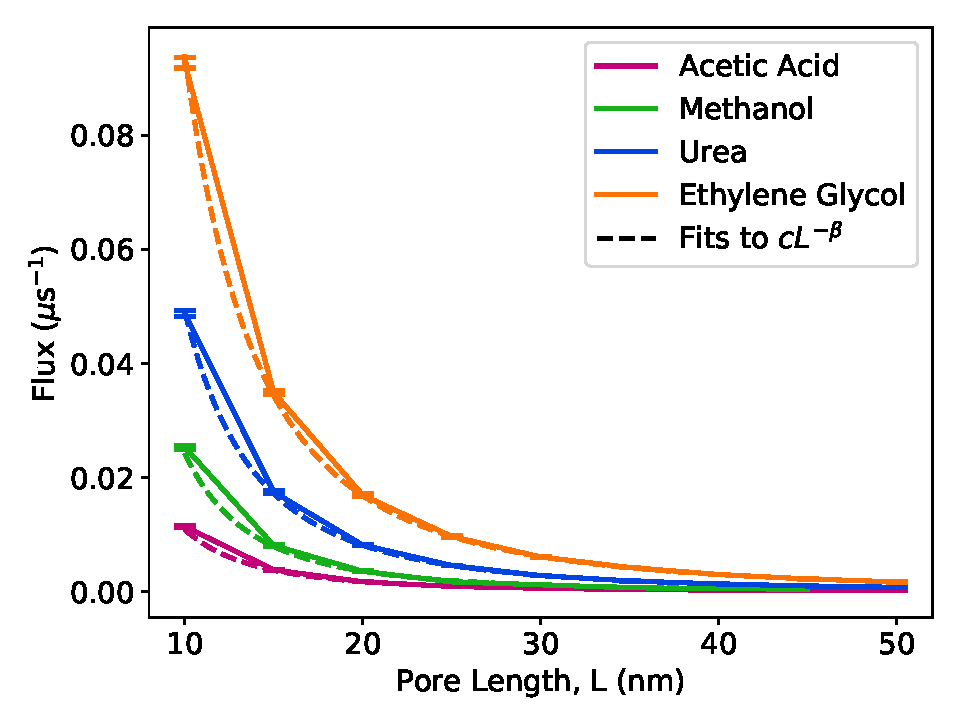
\includegraphics[width=\textwidth]{flux_curves.pdf}
  \caption{Fits to $cL^{-\beta}$}\label{fig:flux_curves_regular}
  \end{subfigure}
  % BJC: could use better color scheme. Maybe outline hurst parameters
  \begin{subfigure}{0.325\textwidth}
  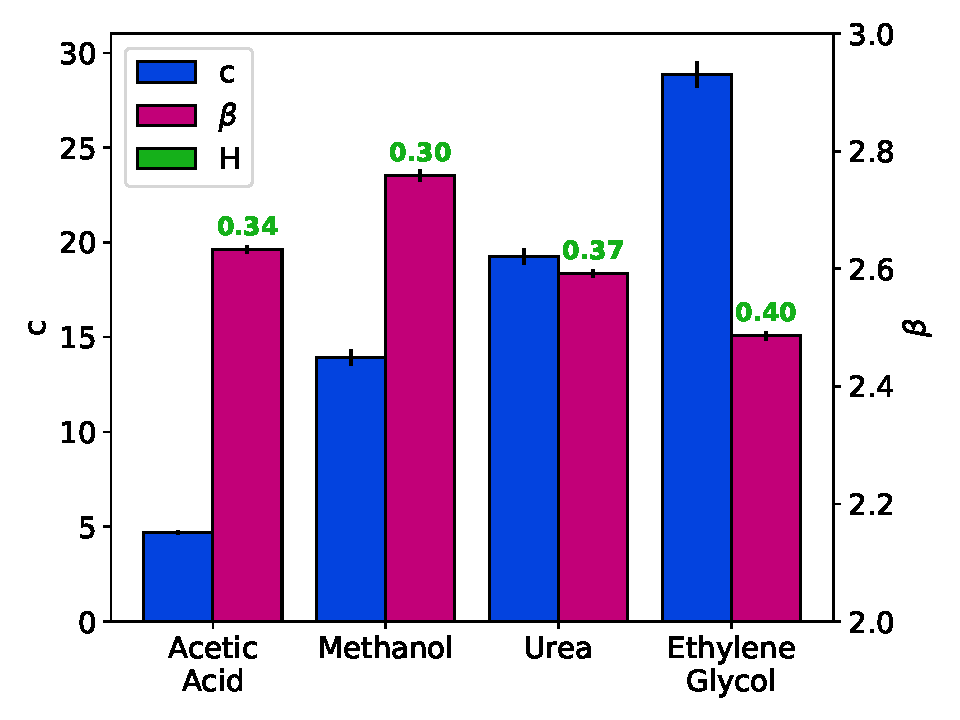
\includegraphics[width=\textwidth]{flux_parameters.pdf}
  \caption{}\label{fig:flux_parameters}
  \end{subfigure}
%  \begin{subfigure}{0.475\textwidth}
%  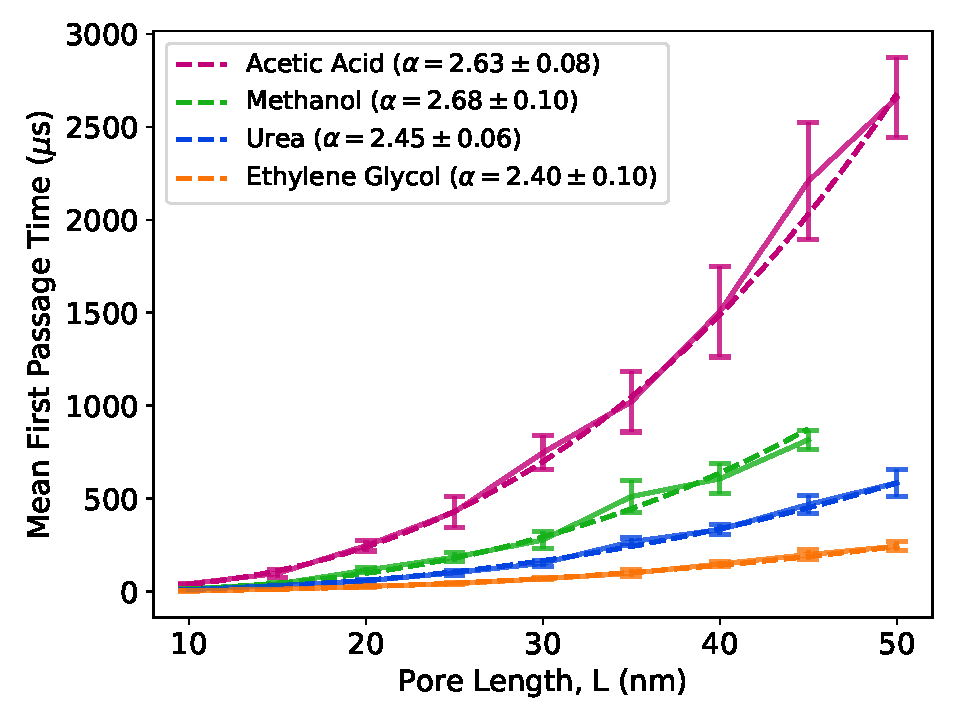
\includegraphics[width=\textwidth]{mfpt_curves.pdf}
%  \caption{}\label{fig:mfpt_curves}
%  \end{subfigure}
  %BJC: going out to 3 decimal places seems silly
  %BJC: might get closer to beta=2 if I use different curve fitting technique than fitting line to log-log
  \begin{subfigure}{0.325\textwidth}
  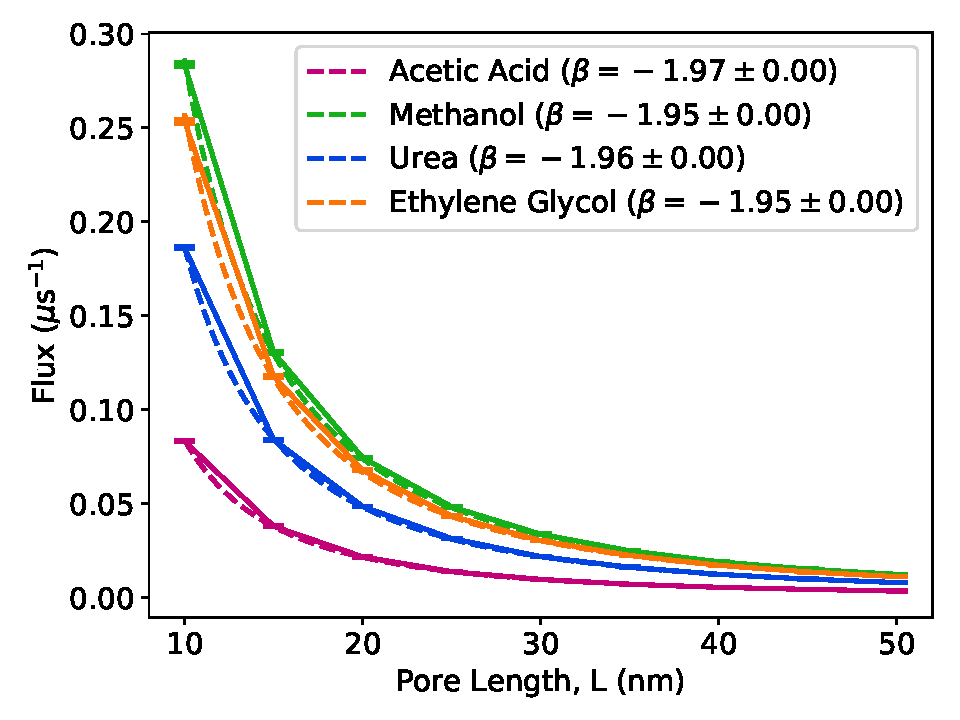
\includegraphics[width=\textwidth]{flux_curves_brownian.pdf}
  \caption{Fixed $H=0.5$}\label{fig:flux_curves_brownian}
  \end{subfigure}
%  \begin{subfigure}{0.475\textwidth}
%  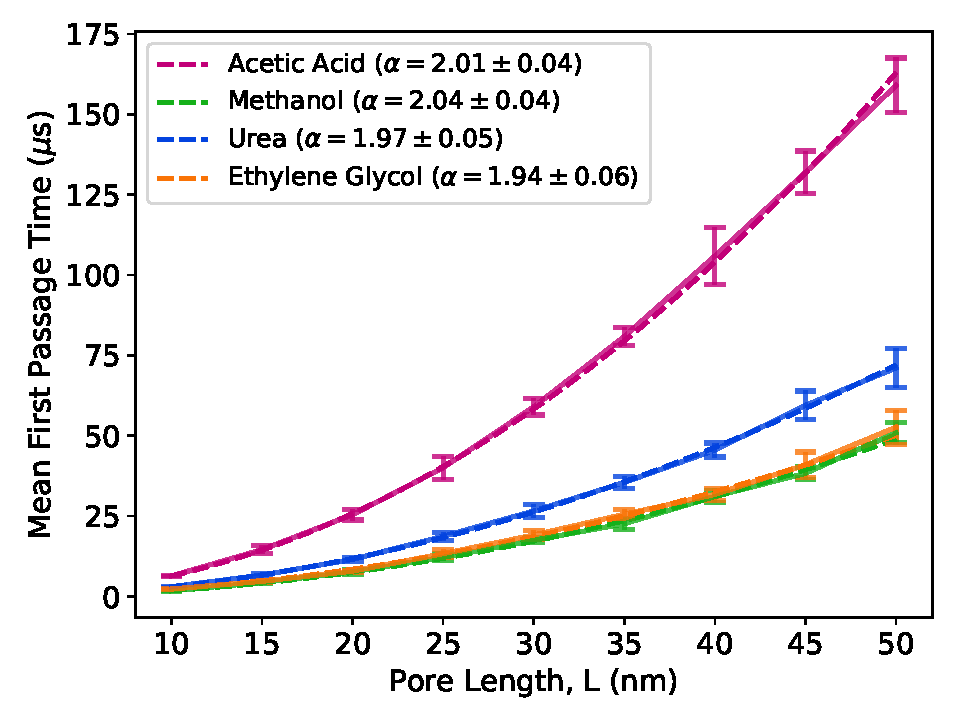
\includegraphics[width=\textwidth]{mfpt_curves_brownian.pdf}
%  \caption{}\label{fig:mfpt_curves_brownian}
%  \end{subfigure}
  \caption{(a) The single particle solute flux decays with increasing pore length. 
  Solutes with high MSDs have higher fluxes. (b) We fit the single particle solute flux 
  versus pore length, $L$, to a power law function of the form $cL^{-\beta}$ (dashed 
  lines in (a)). Solutes with higher fluxes have higher values of $c$. Solutes with 
  smaller Hurst parameters, $H$, have larger values of $\beta$. (c) If we remove 
  correlation between hops (set $H$=0.5), the flux increases significantly and 
  $\beta$ is constant at about 2 for all solutes independent of dwell distribution
  parameters.}\label{fig:flux_curves}
  \end{figure}
  
  % Partially in methods?
  The power law decay of the flux with pore length implies the following relationship
  for selectivity via substitution of Equation~\ref{eqn:flux_decay} into 
  Equation~\ref{eqn:selectivity}:
  \begin{equation}
  S_{ij}(L) = \bigg(\frac{c_i}{c_j}\bigg)L^{(\beta_i - \beta_j)}
  \label{eqn:selectivity_ratio}
  \end{equation}
  
  In Figure~\ref{fig:selectivity}, we plot Equation~\ref{eqn:selectivity_ratio} for pore
  lengths ranging from those studied in Figure~\ref{fig:flux_curves} to macroscopic-length
  pores. Greater differences in $\beta$ values leads to selectivities that are stronger 
  functions of pore length. For $(c_i / c_j)=1$, LLC membranes will be more selective
  towards passage of solutes with lower $\beta$ values versus those with high $\beta$ values.
  When $\beta$ values are equal, as is the case for uncorrelated motion, selectivity only
  depends on the pre-factors, $c$. 
  
  \begin{figure}
  \centering
  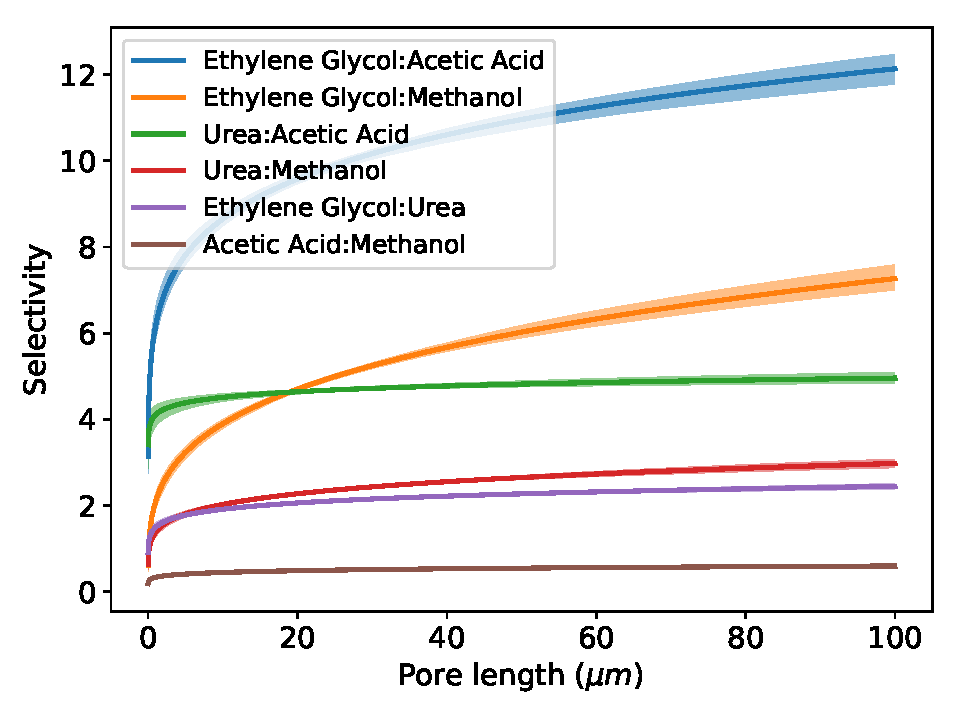
\includegraphics[width=0.5\textwidth]{selectivity.pdf}
  \caption{The selectivity of 2 species changes monotonically with pore length. The
  strength of dependence on pore length depends on the difference between $\beta$ values.}
  \label{fig:selectivity}
  \end{figure}
  
  Out of the solutes studied, the data suggests that this particular LLC membrane 
  would be most useful for selectively separating ethylene glycol from methanol and 
  acetic acid. 
  %It also shows reasonable selectivity of Urea over acetic acid.  
  Ethylene glycol has the highest $c$ value and the lowest $\beta$ value. The high
  value of $c$ itself greatly enhances its selective passage. Even more importantly,
  the relatively large difference between its $\beta$ value and those of methanol 
  and acetic acid give rise to a strong pore length dependence. The selectivity is
  enhanced as the pore length increases at the cost of lower solute flux, a 
  phenomenon ubiquitous in polymer separations membranes.~\cite{geise_water_2011}

  Of course, this approach to modeling LLC membrane selectivity neglects a number of
  factors that influence real-world aqueous membrane separations. The most glaring is 
  that we neglected convective flux which should work to increase overall solute flux 
  and lower selectivity (see Equation ~\ref{eqn:solute_flux}). Defects in the pore 
  structure will have a strong influence on solute flux which may exacerbate the length 
  dependence of flux. Even in a perfectly structured membrane, the barrier to pore
  entry from the bulk solution will have its own influence on experimentally observed 
  selectivities. This energetic barrier can be made even worse by foulants deposited on
  the membrane's surface. Therefore, our predictions should be primarily used to 
  identify the most promising types of selective separations for an H\textsubscript{II}
  LLC membrane made from a specific monomer.
  %BJC: though about mentioning fouli
  
  
    Neglects concentration polarization, membrane defects and fouling.

%  BJC4: Uncomment to see MFPT curves
%  \begin{figure}
%  \centering
%  \begin{subfigure}{0.325\textwidth}
%  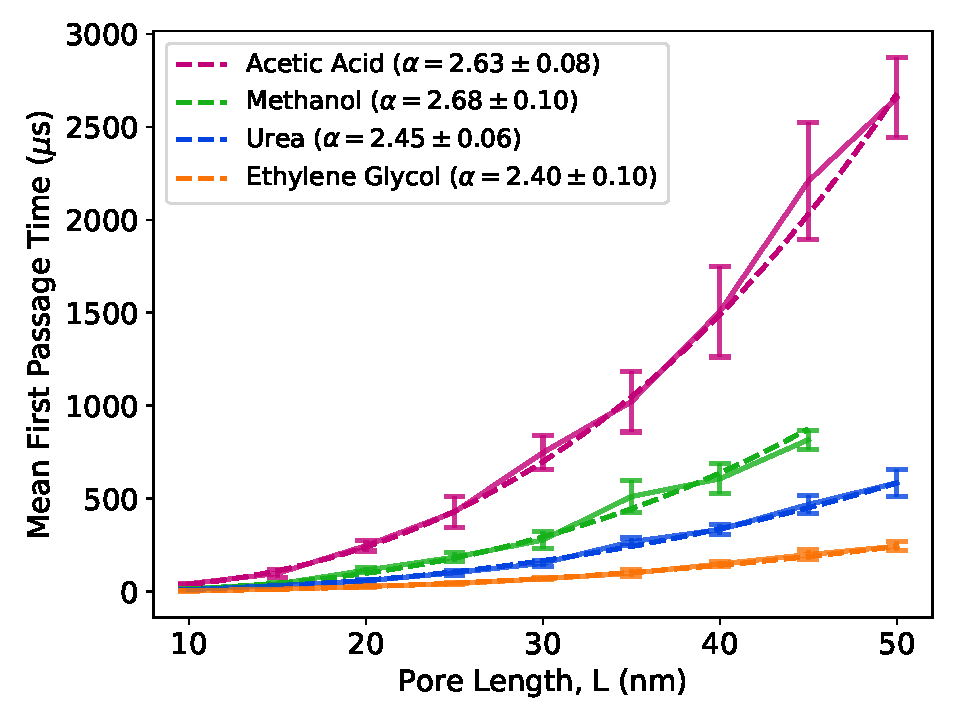
\includegraphics[width=\textwidth]{mfpt_curves.pdf}
%  \caption{Correlated Hops}\label{fig:mfpt_curves_regular}
%  \end{subfigure}
%  \begin{subfigure}{0.325\textwidth}
%  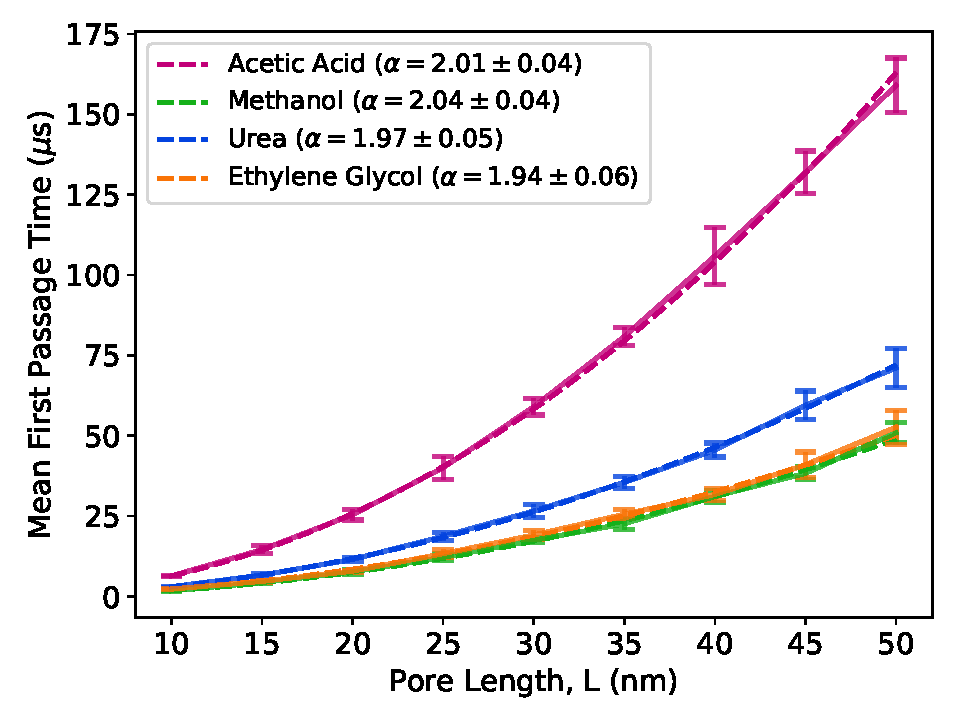
\includegraphics[width=\textwidth]{mfpt_curves_brownian.pdf}
%  \caption{Uncorrelated Hops}\label{fig:mfpt_curves_brownian}
%  \end{subfigure}
%  \begin{subfigure}{0.325\textwidth}
%  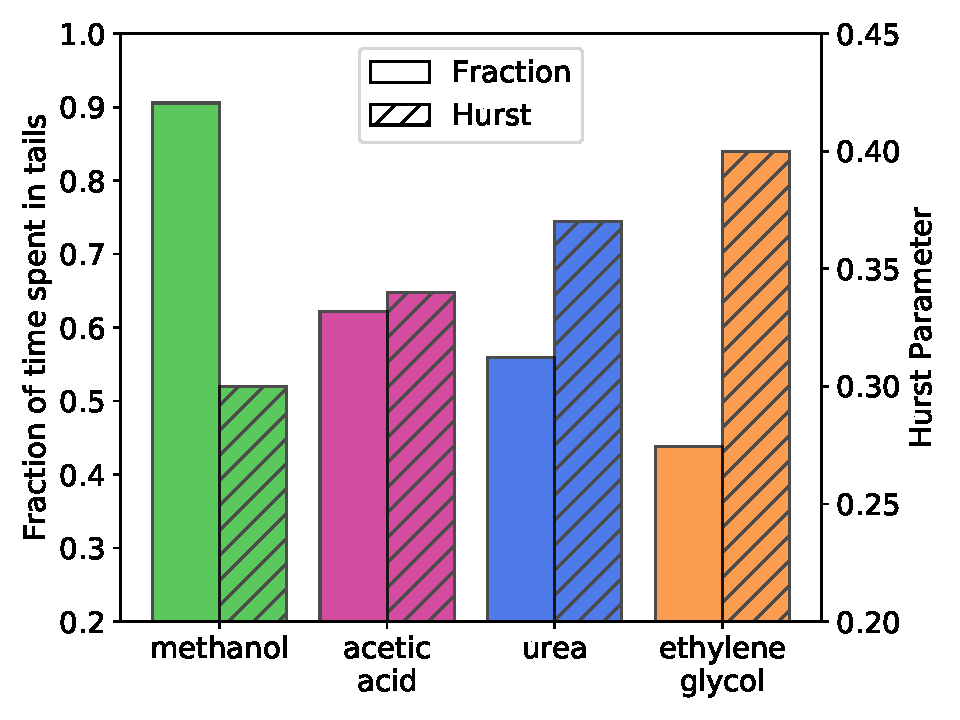
\includegraphics[width=\textwidth]{frac_pore.pdf}  % This figure might fit in earlier
%  \caption{}\label{fig:frac_pore}
%  \end{subfigure}
%  \caption{(a) We fit the MFPT versus pore length to a function of the form $cL^{\alpha}$. 
%  The MFPT grows super-linearly with increasing pore length. Solutes with lower MSDs have
%  higher MFPTs. (b) If we remove correlation between hops, the MFPTs reduce significantly
%  and the growth exponent stays constant at 2 for all solutes independent of dwell
%  distribution parameters. Higher degrees of anti-correlation (lower $H$) lead to higher
%  growth exponents. (c) Solutes that spend a large fraction of their time in the tails tend
%  to have larger Hurst parameters.}\label{fig:mfpt_curves}
%  \end{figure}
  
%  In Figure~\ref{fig:frac_pore}, we show that solutes which spend more time in the tails
%  tend to have lower Hurst parameters. The densely packed, viscoelastic alkane chains 
%  bounce solutes between them, severely limiting their mobility. Designing LLC membranes
%  that can control or prevent the partition of solutes into the tails may offer the highest
%  returns on membrane performance.
  
  %BJC: can make design suggestions by trying to decrease anticorrelation by x
  
%  In this section, we use our most promising models to predict solute flux 
%  through a theoretical 50 nm channel. For our comparisons to MD, using a truncated
%  power law distribution is an obvious choice. However, given that extremely
%  long dwells are a rare event, it is possible that studying a much larger set of 
%  solutes will fill in the tail of the pure power law PDF. Regarding hop length 
%  distributions, the generality of L\'evy stable distributions is powerful, but the
%  lack of exact methods for simulation of fractional L\'evy motion reduces it's 
%  accuracy and computational tractability. Treating the dynamics as fractional 
%  Brownian motion is probably sufficient unless the L\'evy index, $\alpha_h$, is 
%  well below 2.
%  
%  Choosing which model to use for long timescale projections is not entirely obvious
%  without experimental data to compare with. 
  
%  We projected the long timescale behavior using this model. 

  \section{Conclusions}
  
  % BJC4: Say something about pore entry and exit as an improvement to the model
  
  We have tested two different mathematical frameworks for describing solute
  motion in an H\textsubscript{II} phase LLC membrane. The values obtained for
  the parameters when fitting the models to the time series data offer important
  mechanistic insight on the molecular details of transport.
  Subordinated fractional Brownian and L\'evy motion have a nice theoretical 
  foundation in the anomalous diffusion literature. Our single mode model
  quantifies and allows comparison of the hopping and trapping behavior 
  between solutes. A two mode model that describes dynamics based on whether
  a solute is in or out of the pore region allows us to break down individual
  solute motion into the two distinct regimes and we showed that solute motion is
  clearly restricted while in the tail region. Our Markov state-dependent dynamical
  model uses explicitly defined trapping mechanisms and gives a nice description 
  of transitions between these observed states, the equilibrium distribution of 
  solutes among states as well as the type of stochastic behavior shown in each 
  state. However, it doesn't accurately portray correlated time series behavior
  leading to overpredicted MSDs.
  
  %MRS4: test/train in order to show power?
  We believe that our models have moderate predictive power. 
  %MRS4: be more precise on how superior is quantified below.
  The anomalous
  diffusion model has superior performance to the MSDDM. Both 1 and 2 mode 
  sFBM and sFLM with truncated power law distributions predict MSDs close 
  to those simulated with MD while the MSDDM significantly over-predicts MSDs.
  One might have more success using the MSDDM with a system that exhibits
  infrequent transitions between states.

  Our mathematical models help us think about how to design LLC monomers for 
  solute-specific separations by forcing us to think in terms of controlling 
  solute trapping. The anomalous diffusion model is quite flexible because it
  does not require knowledge of specific trapping mechanisms. Screening a set
  of solutes and applying the anomalous diffusion model can help uncover
  trapping mechanisms by forcing the scientist to identify features common 
  to solutes with long or short hop lengths and dwell times. The MSDDM is a 
  powerful way to characterize explicit trapping mechanisms. Although its
  predictive power is inferior to the anomalous diffusion model, it clearly
  partitions a trajectory into discrete mechanisms and quantifies their
  relative dominance in the real system. For example, it is clear that 
  sodium ion association is primarily responsible for trapping urea while 
  hydrogen bonding dominates ethylene glycol. If one re-designs an LLC monomer
  to eliminate one source of trapping, 
  %MRS4: by what mechanisms are high selectivities possible?
  then high selectivities are possible.
  
%  Properly parameterizing
%  and simulating the correlation structure of the time series is very important. 
%  Based on physical intuition, we assumed the correlation to be a consequence of 
%  a fractional process however, autoregressive techniques may offer a more flexible
%  approach.
% Both models describe the trapping mechanism in
%  different ways. The anomalous diffusion model does not consider mechanisms but
%  insight into the length of entrapment
%  
%  The anomalous diffusion gives clues to the type 
%  of functionality that leads to long dwell times. It is readily apparent that solute 
%  
%  One must consider how to control them and 
%  a solute's preference towards the pore or tail region. 
%  They can dissect solute movement down to their 
%  individual positional fluctuations and give information about the influence 
%  of the surrounding chemical environment. 
%
%  
%  Combined with qualitative studies of solute transport to aid in model construction,
%  our stochastic modeling framework can be used to quantitatively dissect the dynamic
%  behavior of solutes in LLC membranes. Our work demonstrates that when designing a membrane for a 
%  specific separation, one must consider the types of trapping mechanisms that 
%  may play a role in transport, how solutes partition in the membrane,
  
  
  \section*{Supporting Information}

  Detailed explanations and expansions upon the results and procedures mentioned in
  the main text are described in the Supporting Information. This information is
  available free of charge via the Internet at http://pubs.acs.org.

  \section*{Acknowledgments}
  %MRS: add people who contributed non-author level ideas. 
  %MRS3: add specific info for PRF and GAANN
  %BJC3: I don't know the PRF info. I wrote GAANN as I did on the last paper which is what Rob Davis told me to do
  %MRS4: I willō track down the PRF grant number (if typical)
  This work was supported in part by the ACS Petroleum Research Fund grant \#59814-ND7
  and the Graduate Assistance in Areas of National Need (GAANN)
  fellowship which is funded by the U.S. Department of Education.
  Molecular simulations were performed using the Extreme Science and
  Engineering Discovery Environment (XSEDE), which is supported by National
  Science Foundation grant number ACI-1548562. Specifically, it used the Bridges
  system, which is supported by NSF award number ACI-1445606, at the Pittsburgh
  Supercomputing Center (PSC). This work also utilized the RMACC Summit supercomputer,
  which is supported by the National Science Foundation (awards ACI-1532235 and
  ACI-1532236), the University of Colorado Boulder, and Colorado State
  University. The Summit supercomputer is a joint effort of the University of
  Colorado Boulder and Colorado State University.

  \clearpage

  \bibliographystyle{ieeetr}
  \bibliography{stochastic_transport}

  \newpage

  \section*{TOC Graphic}

\end{document}

% LocalWords:  solute MSDs solutes solute's LLC BJC nanoporous maginn Lyotropic
% LocalWords:  micropollutants LLCs amphiphilic mesophases feng Bicontinuous EG
% LocalWords:  permeability hatakeyama zhou resel selectivities Edisonian CTRW
% LocalWords:  subdiffusive timescale timescales subdiffusion FBM RWF metzler
% LocalWords:  jeon neusius pdf Sokolov ony MSD MSMs chodera MSM AcOH URE MeOH
% LocalWords:  Hbonding hbonds hbond GROMACS berendsen gromacs der spoel hess
% LocalWords:  wt Na GA carboxylate Parrinello Rahman barostat rescale msd dt
% LocalWords:  superdiffusive EB sFBM min Hurwitz factoid MLEs autocovariance
% LocalWords:  evy sFLM FLM sFLMcut Dirichlet saiid fbm Stoev Taqqu MLE TODO SI
% LocalWords:  vvvv wehmeyer MSMbuilder pyEMMA featurization Phys Chem bayesian
% LocalWords:  Markovianity MSDDMs MSDDM resampling TBD MSD's CTRWs GCL acf ACH
% LocalWords:  urea's alkane overlayed SFLMcut underpredicted Gaussians HMM PRF
% LocalWords:  params msddm timeseries overpredicted GAANN ACS XSEDE ACI PSC
% LocalWords:  RMACC TOC
